\chapter{Results and conclusion}


In this chapter, we will comment on the results obtained with the algorithms we described in the previous chapters: we will both analyze them individually and compare them with each other. Then we will present our conclusions.


\section{Results}

% Dire cosa vogliamo andare a guardare per capire come fare meglio, se possiamo fare meglio, quindi ci serve una metrica; poi cominci a giustificare i parametri che abbiamo messo nelle simulazioni; dai qualche indicazione operativa e poi inizi a commentare i risultati.

We implemented firstly the ordinary policy gradient descent (\acrshort{pg}), using the formula for the gradient $\nabla_{\boldsymbol \theta} J_\pi (\boldsymbol \theta)$ in equation \eqref{eq:mygradJ}. Then, realizing how slow the convergence was, we decided to implement also the natural policy gradient algorithm (\acrshort{npg}), following equation \eqref{eq:mynatgradJ}. While reaching the same policy (the difference is in the order of $10^{-2}$), the \acrshort{npg} reaches convergence incredibly faster than the \acrshort{pg} algorithm, as we can see from the right panel of \autoref{fig:times}. From the left panel, which reports the same times but in logarithmic scale, we can see that both the two curves are exponentials, with approximately the same rate, but the \acrshort{npg} one has an initial value about $10^{-2}$ times smaller than the \acrshort{pg} one, which considerably reduces the computation time.
% ab^x, cd^x -> log(ab^x), log(cd^x) -> log(a)+xlog(b), log(c)+xlog(d) -> log(b) = log(d), log(a) != log(c)

These two algorithms find a policy that is not completely deterministic: in fact, some states have a stochastic policy over their possible actions. This means that we are on a side of the simplex which represents the policy space, and not in a corner. However, if, given a fault, we follow the actions dictated by the policy, we end up only in states with a deterministic choice of the action to be performed. In particular, an interesting thing to notice is that in the initial state the policy always tells to go to the substation in the middle, like the bisection algorithm. Then, for subsequent substations, the two policies began to differ, giving very different results, as we will see later.

\begin{figure}[t]
    \centering
    \mbox{
        \hspace*{-19.5pt}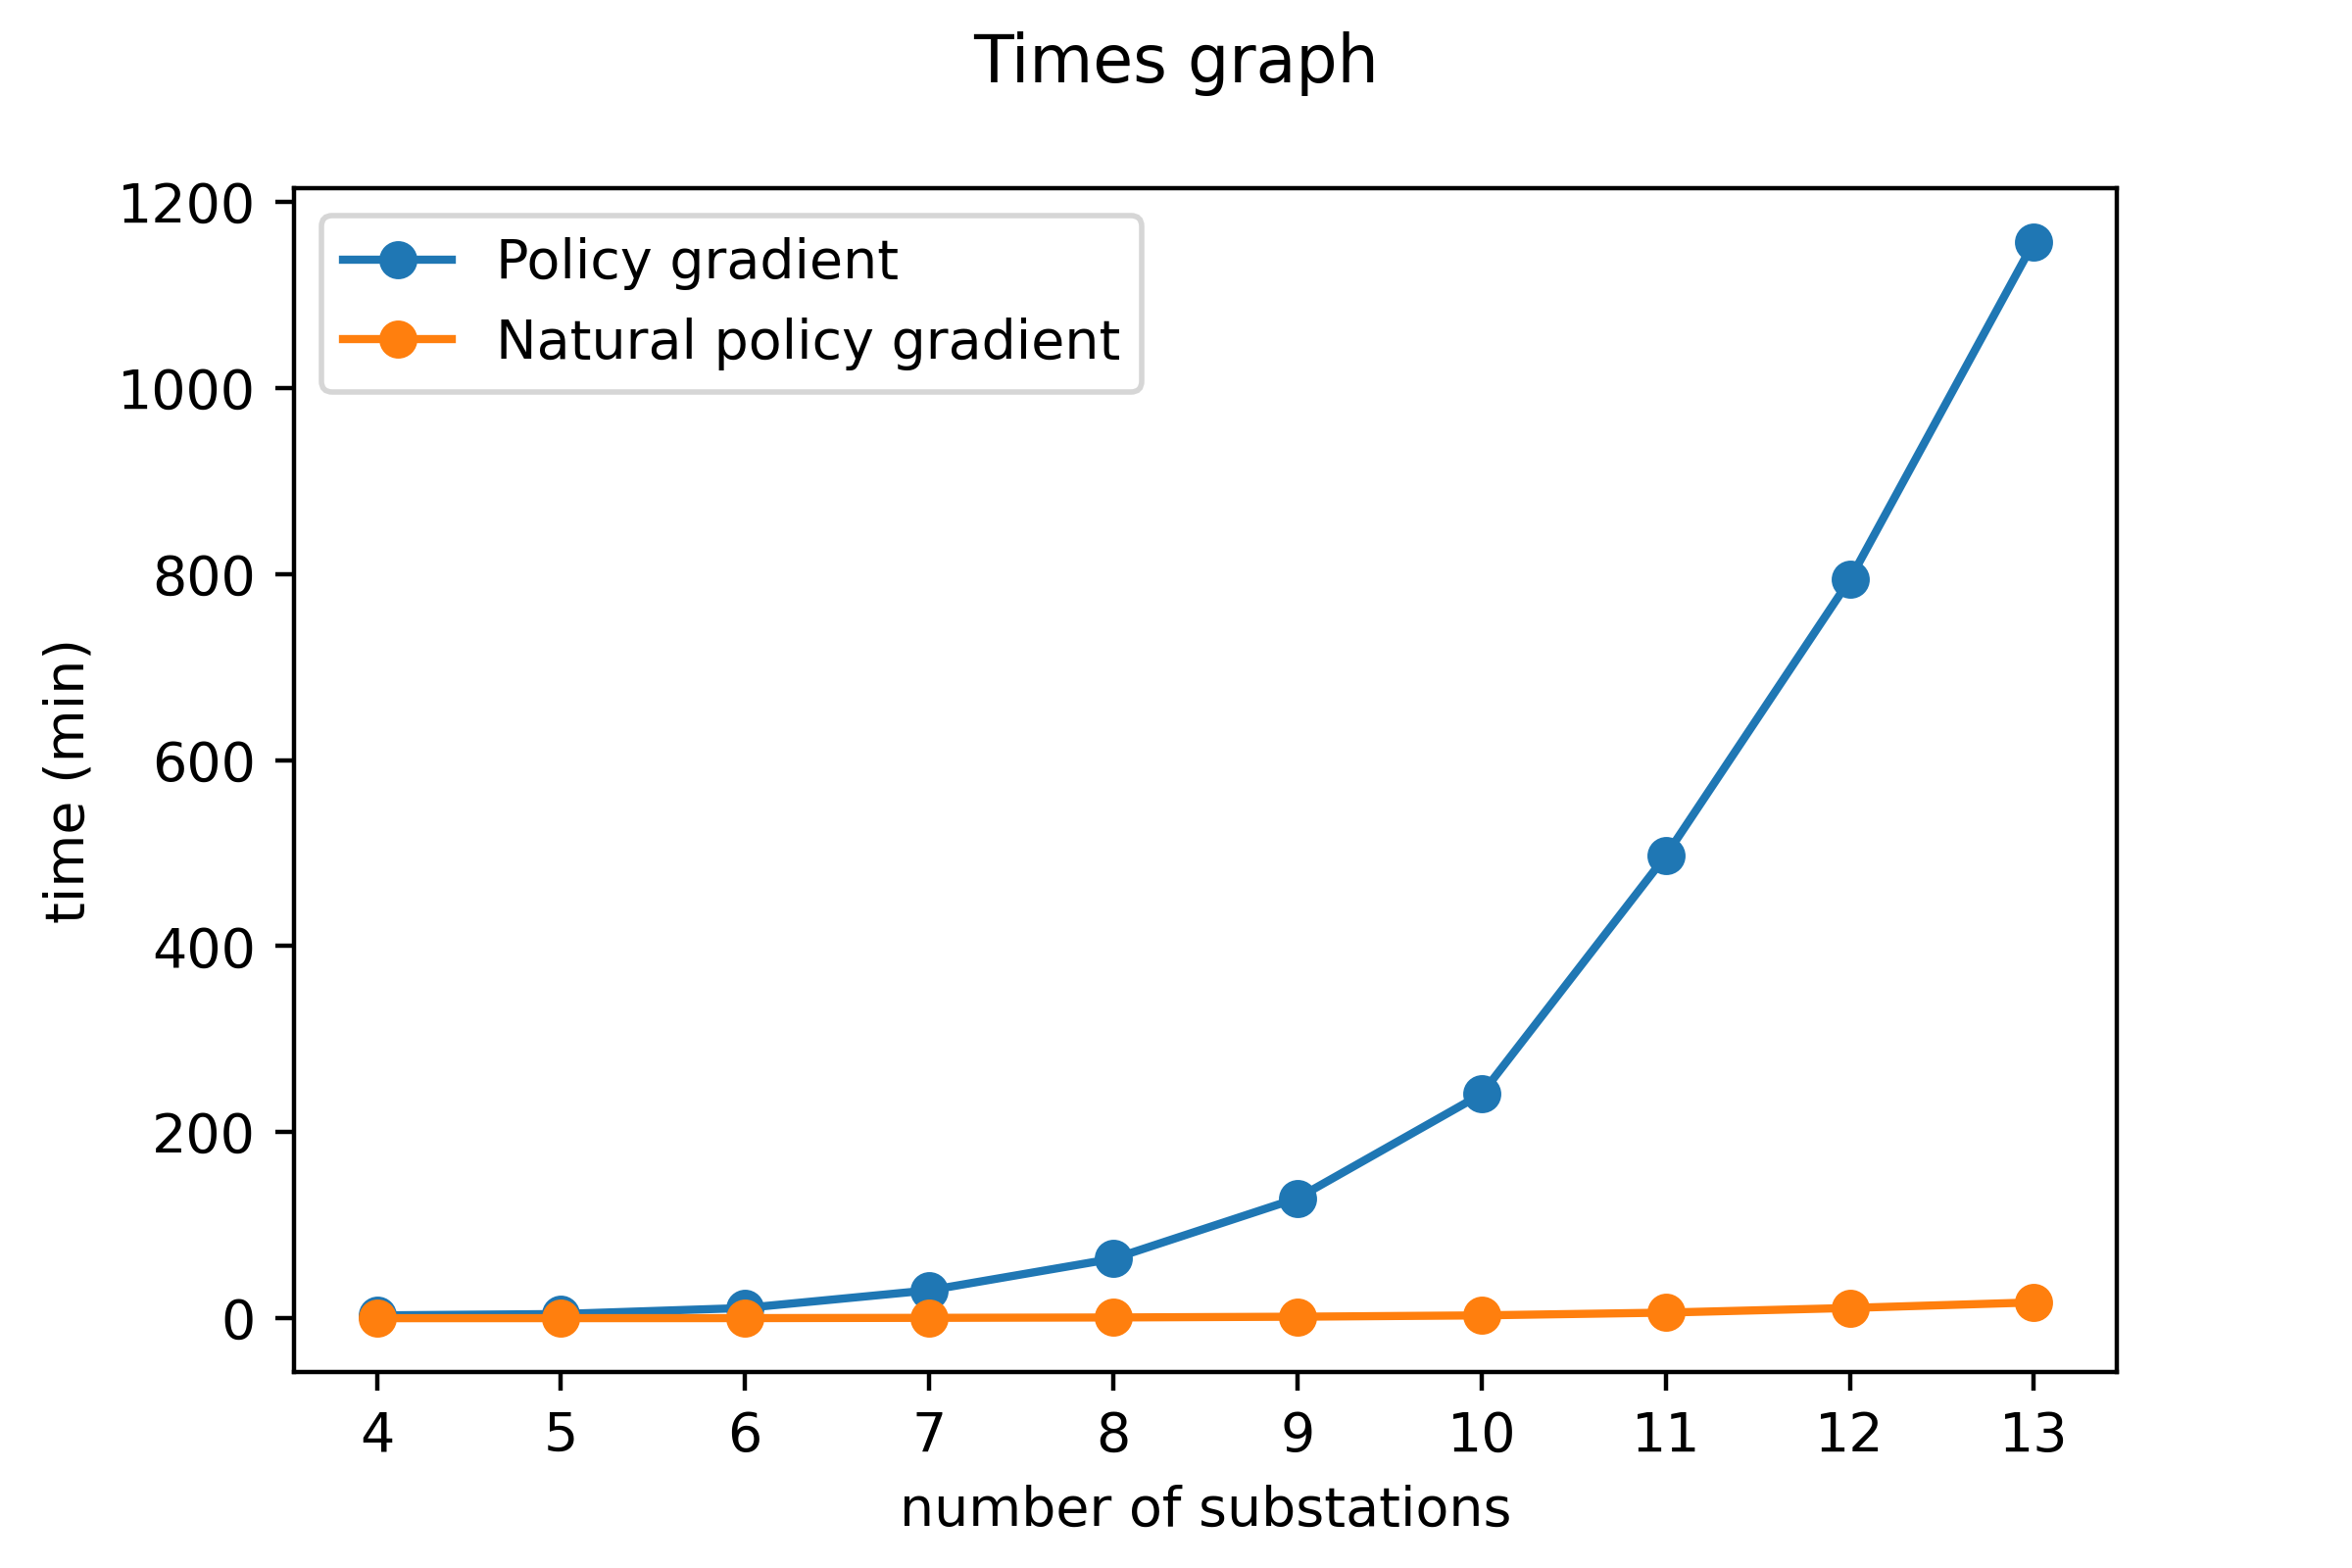
\includegraphics[width=0.55\textwidth]{chapters/figures/times_graph.png}
        \hspace*{-19.5pt}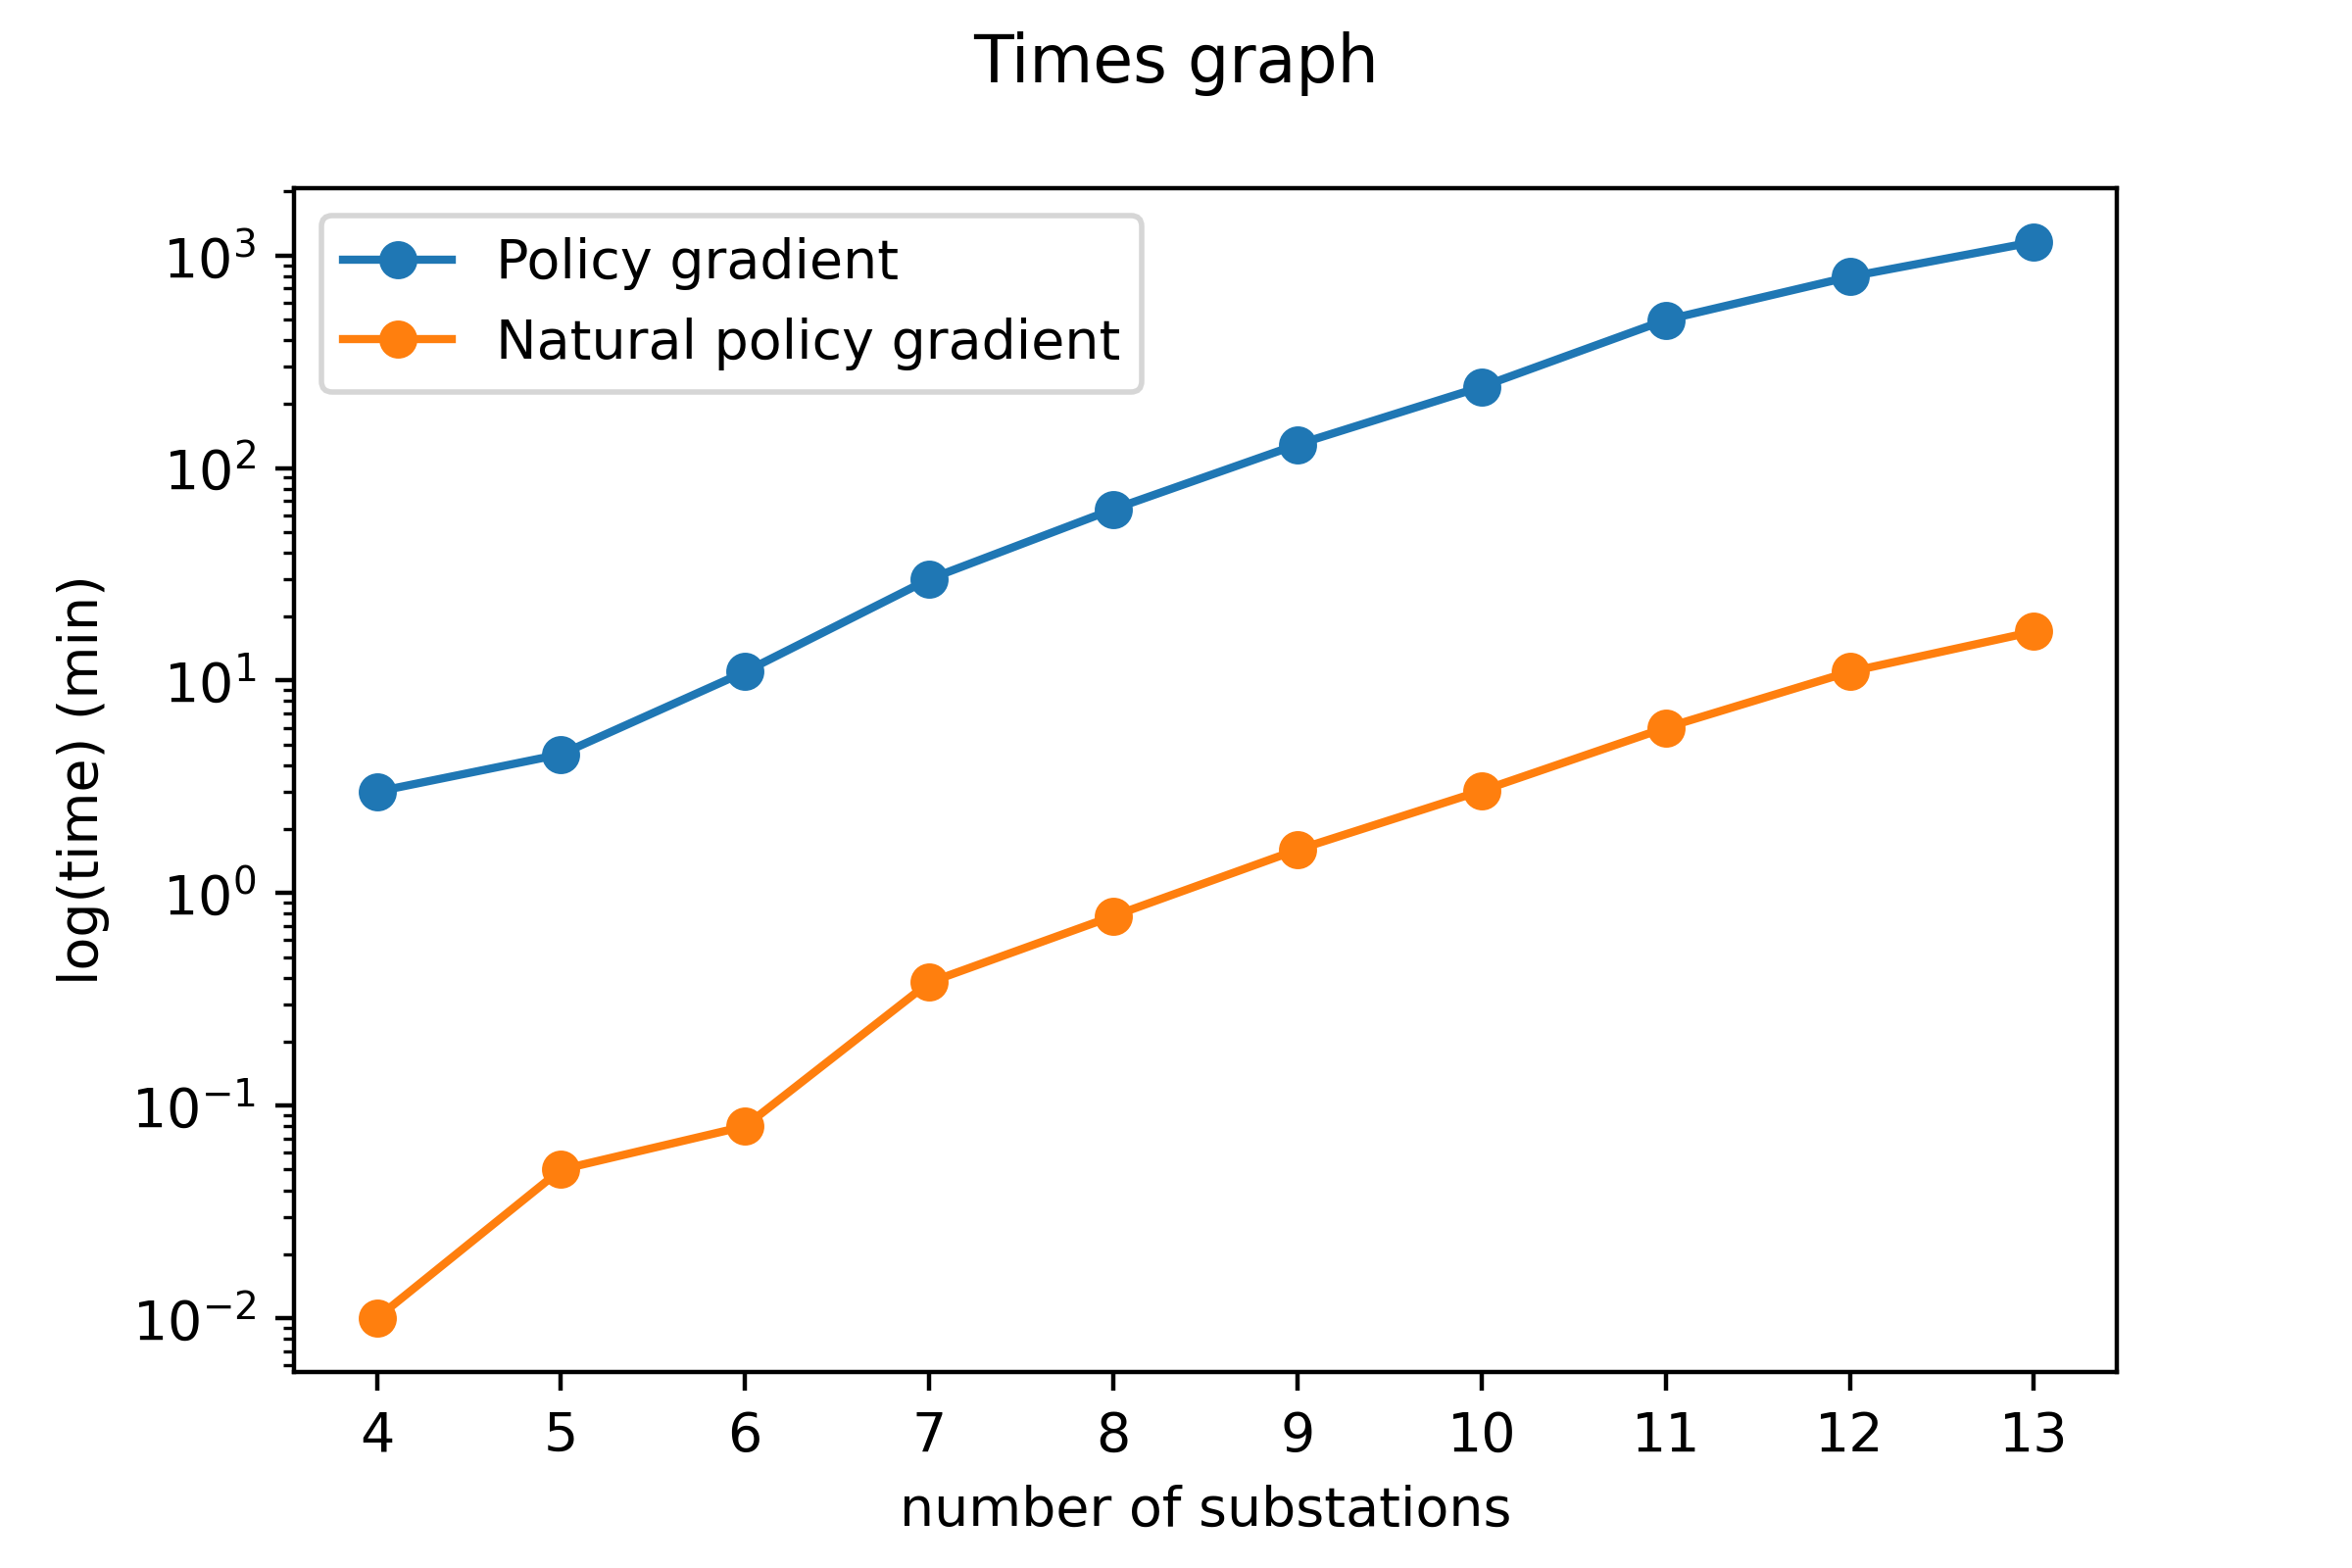
\includegraphics[width=0.55\textwidth]{chapters/figures/times_graph_log.png}
    }
    \caption{Comparison of the times of \acrshort{pg} and \acrshort{npg}. The second figure shows the same times in logarithmic scale.}
    \label{fig:times}
\end{figure}

The first thing to look at in a policy gradient algorithm is whether the gradient descent reached convergence. The first, immediate, check is to see if the error is decreasing. We checked this both for the \acrshort{pg} algorithm and for the \acrshort{npg} algorithm, and both of them were decreasing. In figure \autoref{fig:errors-pg} we can see the plots of the errors for the ordinary policy gradient: in the left panel there is the complete sequence, while in the right panel we zoomed since the error is less than $1$. In figure \autoref{fig:errors-npg} we can see the two plots for the natural policy gradient.

\begin{figure}[htb]
    \centering
    \mbox{
        \hspace*{-19.5pt}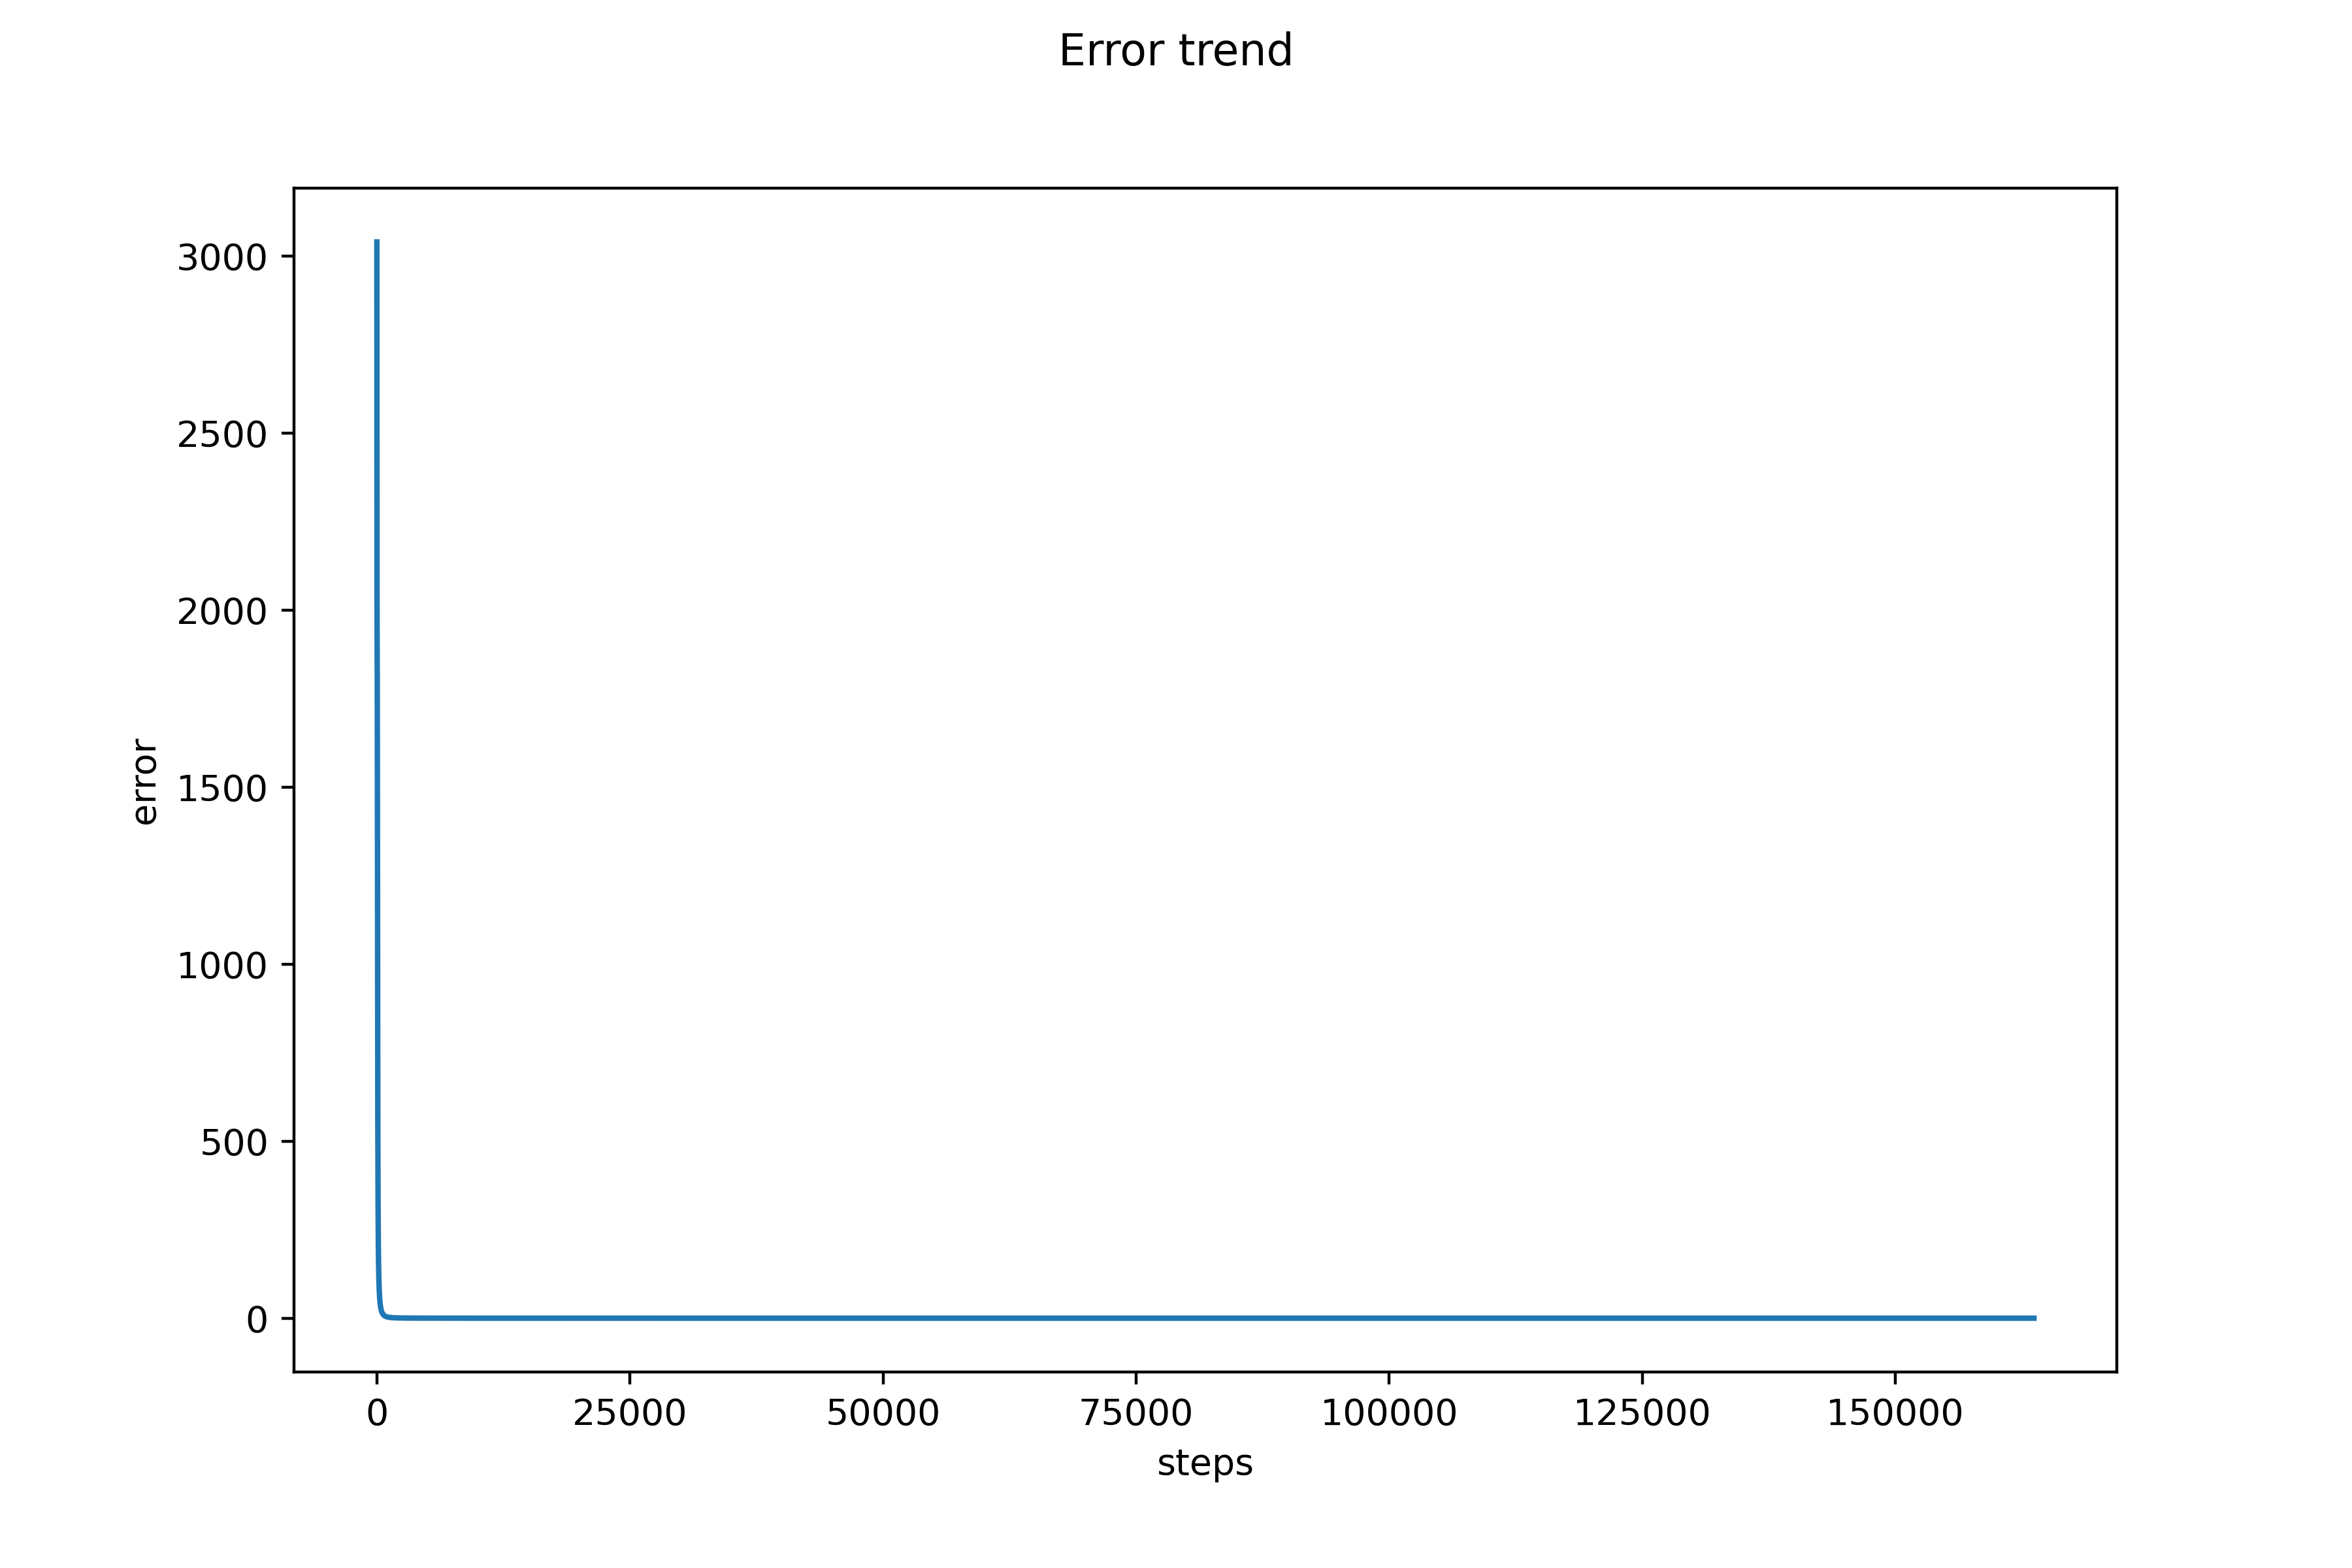
\includegraphics[width=0.55\textwidth]{chapters/figures/errors_PG.png}
        \hspace*{-15pt}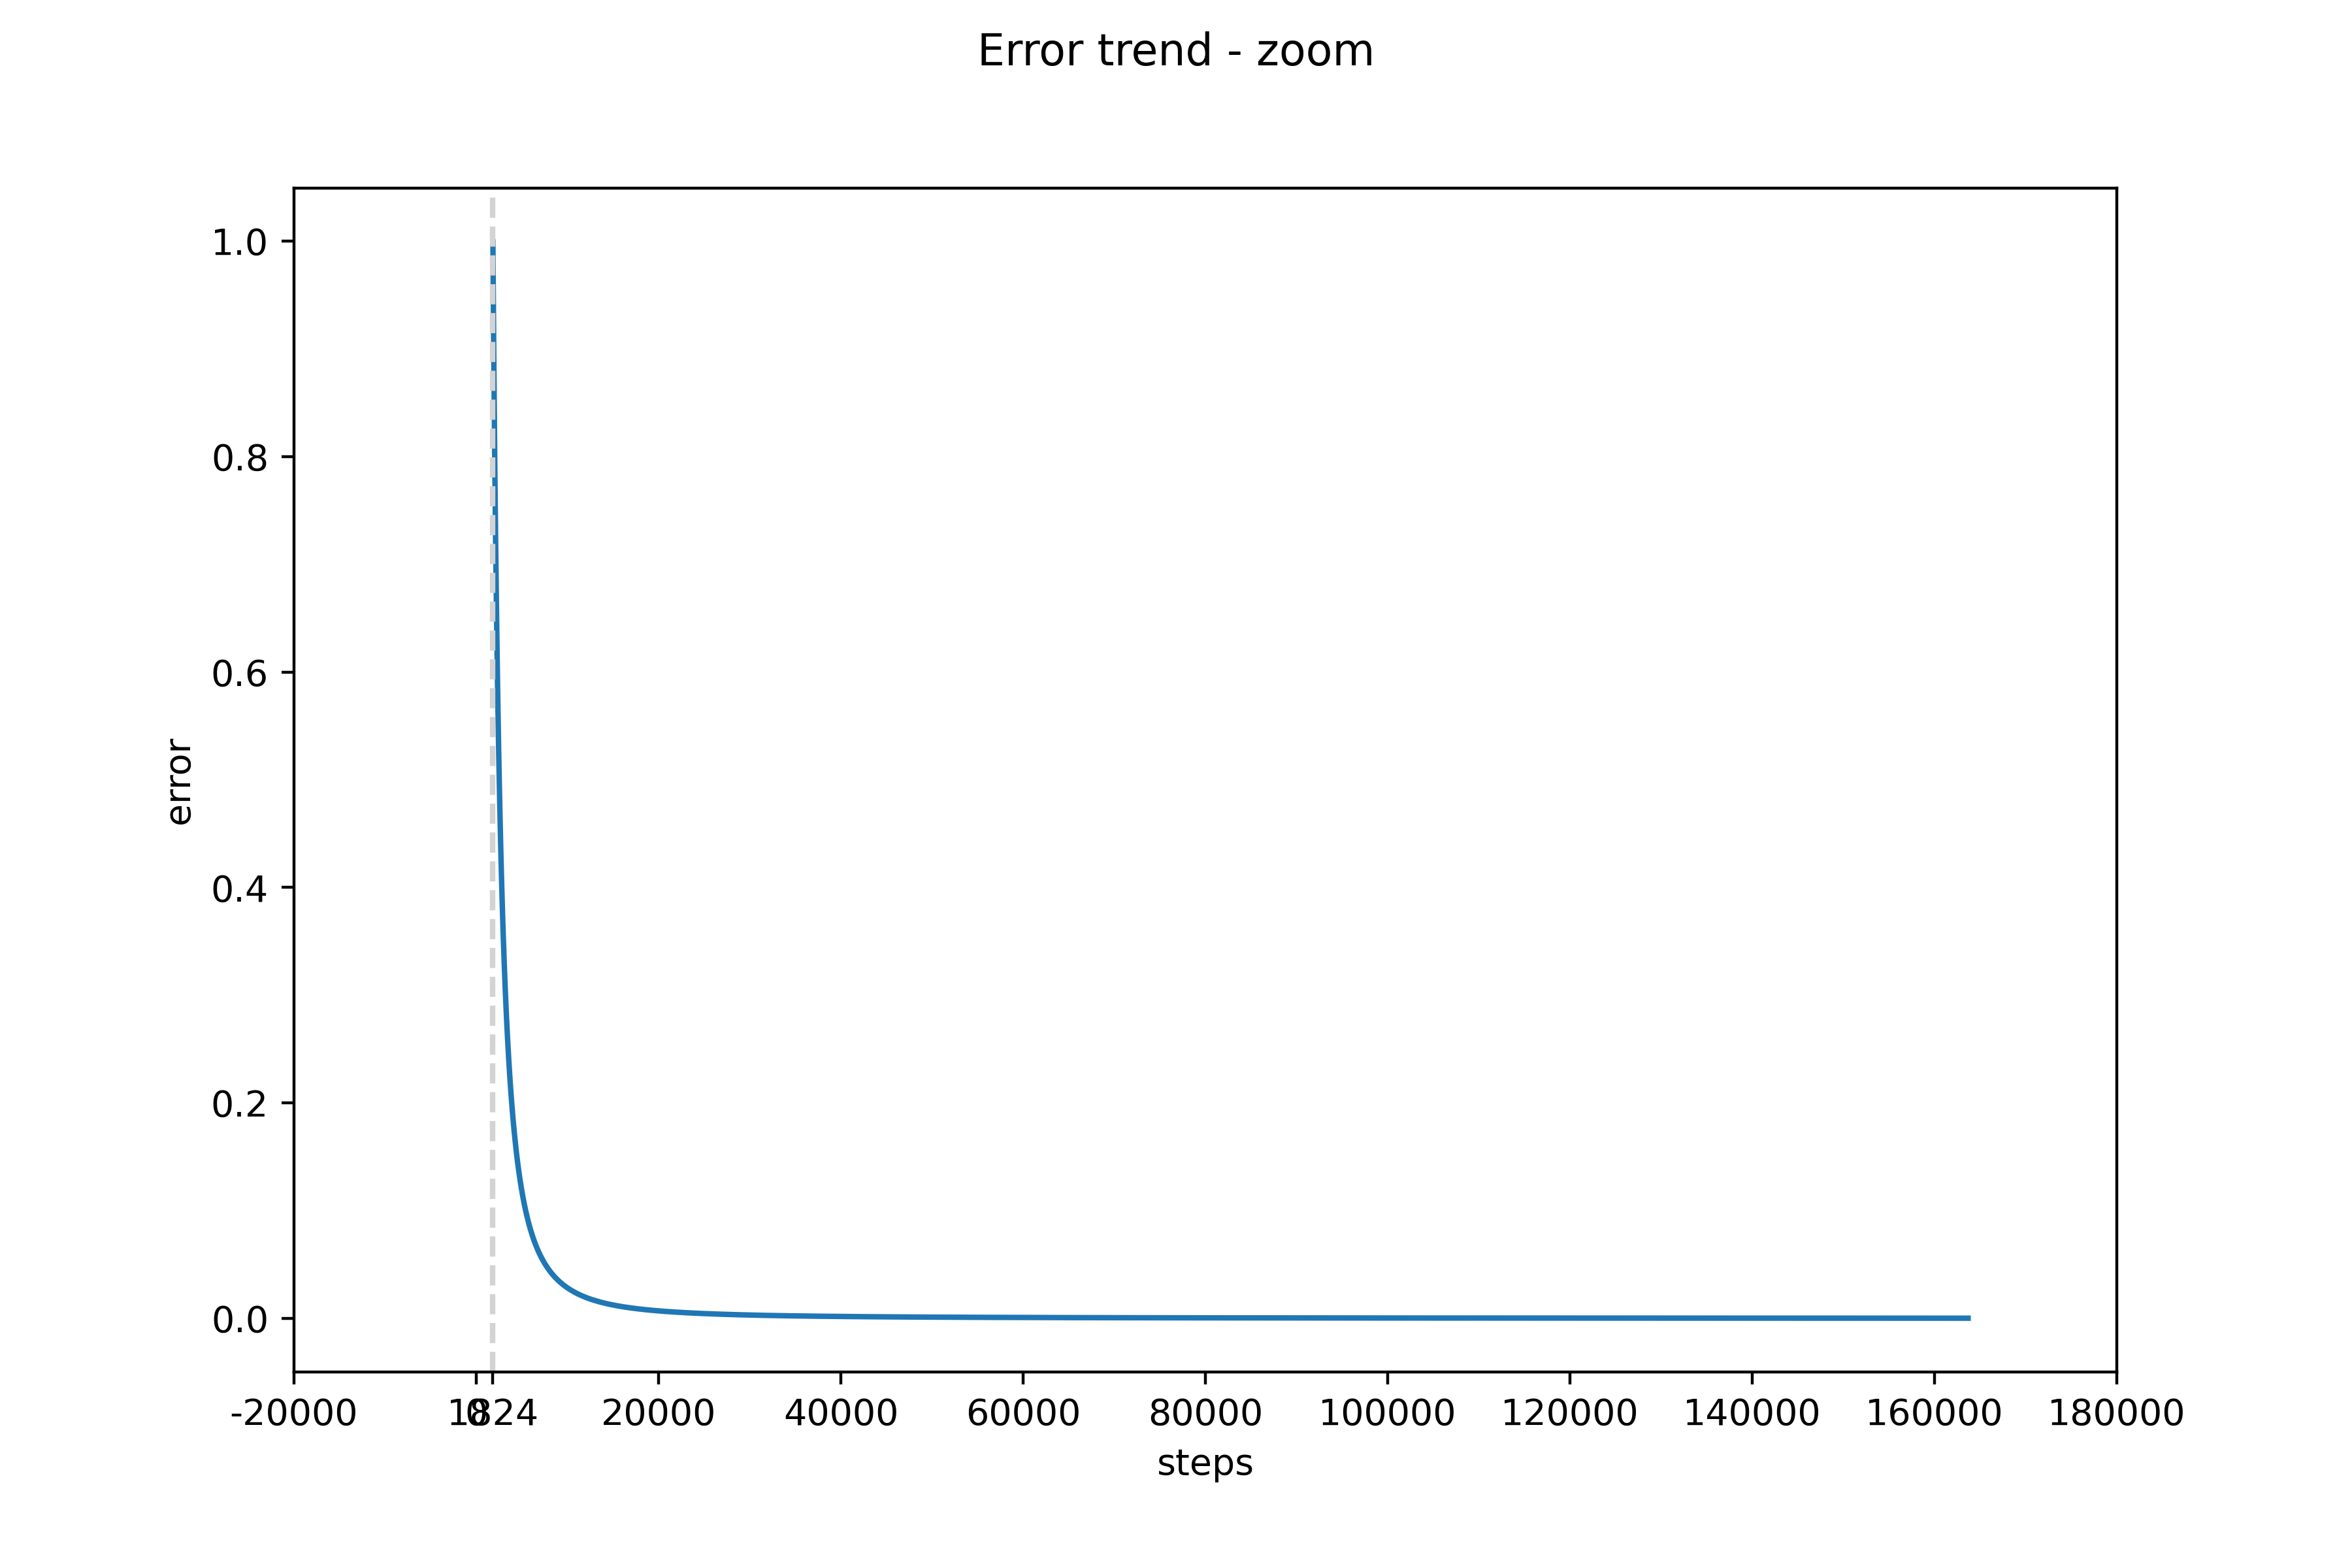
\includegraphics[width=0.55\textwidth]{chapters/figures/errors_zoom_PG.png}
    }
    \caption{\acrshort{pg} errors: they are decreasing, like they should.}
    \label{fig:errors-pg}
\end{figure}

\begin{figure}[htb]
    \centering
    \mbox{
        \hspace*{-19.5pt}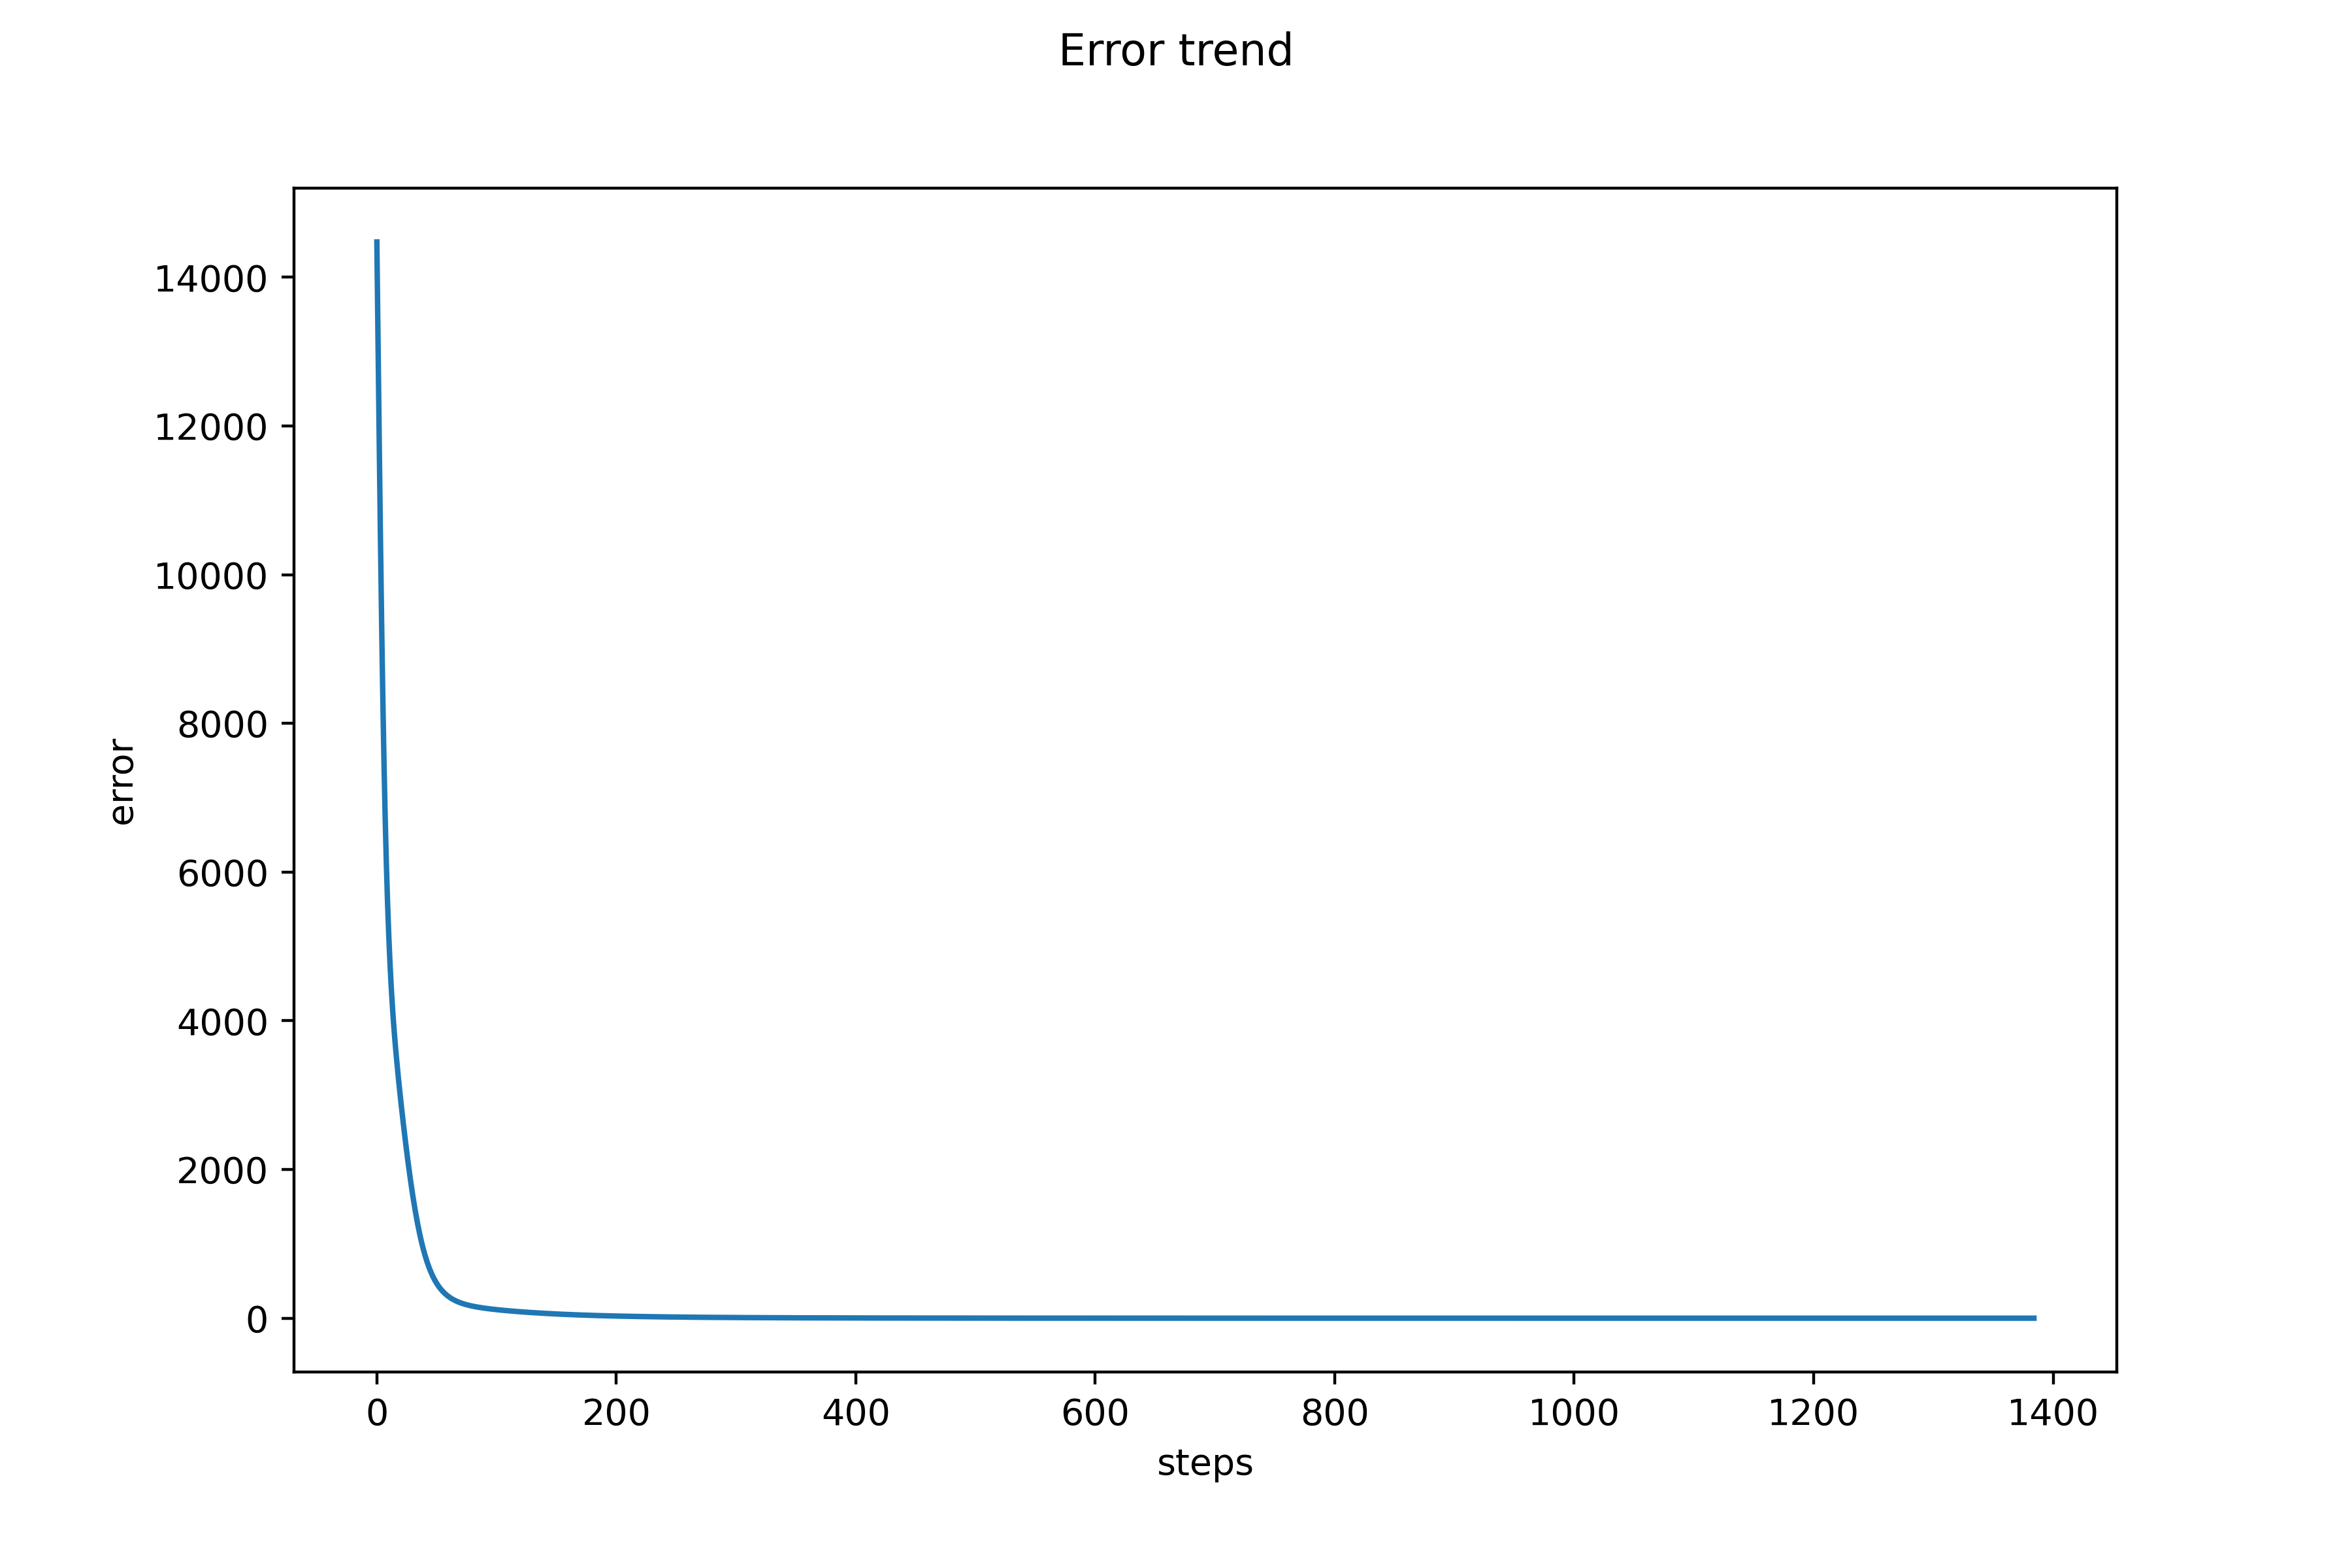
\includegraphics[width=0.55\textwidth]{chapters/figures/errors_NPG.png}
        \hspace*{-15pt}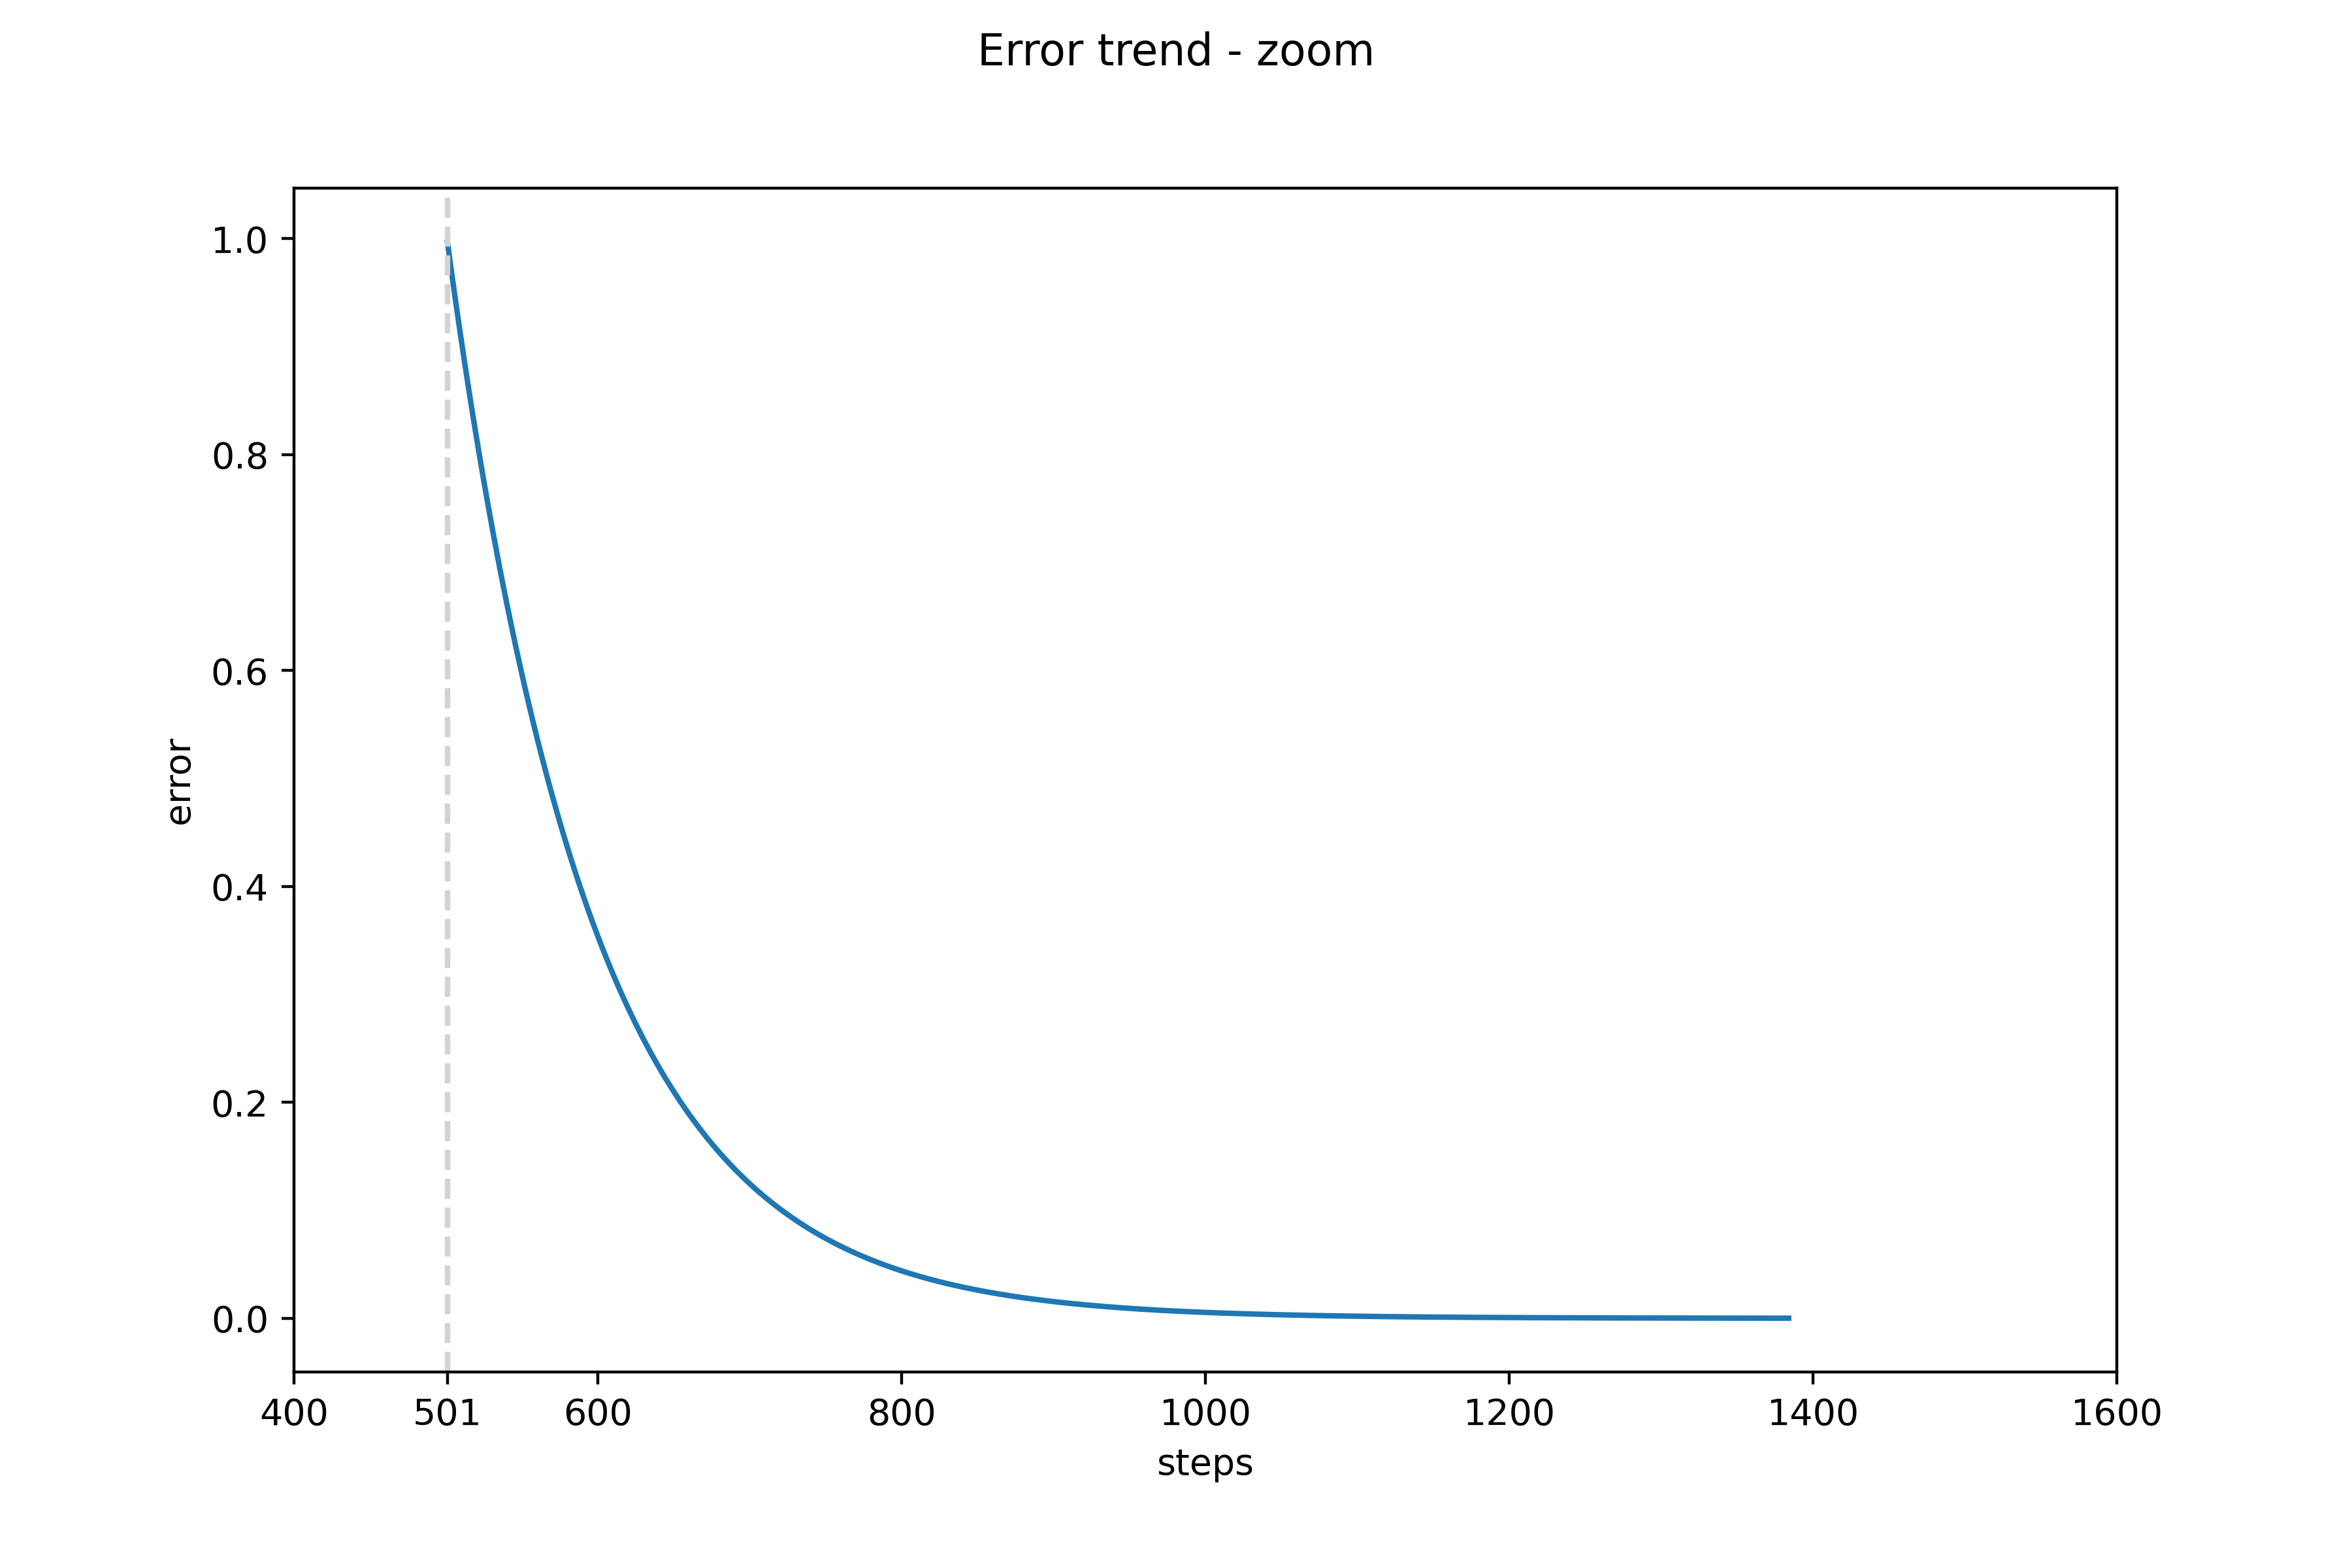
\includegraphics[width=0.55\textwidth]{chapters/figures/errors_zoom_NPG.png}
    }
    \caption{\acrshort{npg} errors: they are decreasing, like they should.}
    \label{fig:errors-npg}
\end{figure}

However, this is not enough to say that the algorithm converged, this is a mere indicator that the gradient descent is indeed following the gradient and moving towards a minimum. Thus, what we did next was to examine the trajectories of the parameters $\boldsymbol \theta$ in the parameters space and the trajectories of the policies $\pi_{\boldsymbol \theta}$ in the policy space. In \autoref{fig:sequence-theta-pg} and \autoref{fig:sequence-policies-pg} we can see them for the \acrshort{pg}, where we selected a specific episode with $5$ initially disconnected substation and the fault among the second and the third substation. In \autoref{fig:sequence-theta-npg} and \autoref{fig:sequence-policies-npg} we can see them for the \acrshort{npg} for the same exact episode.

\begin{figure}[!htp]
    \centering
    \begin{tabular}{cc}
        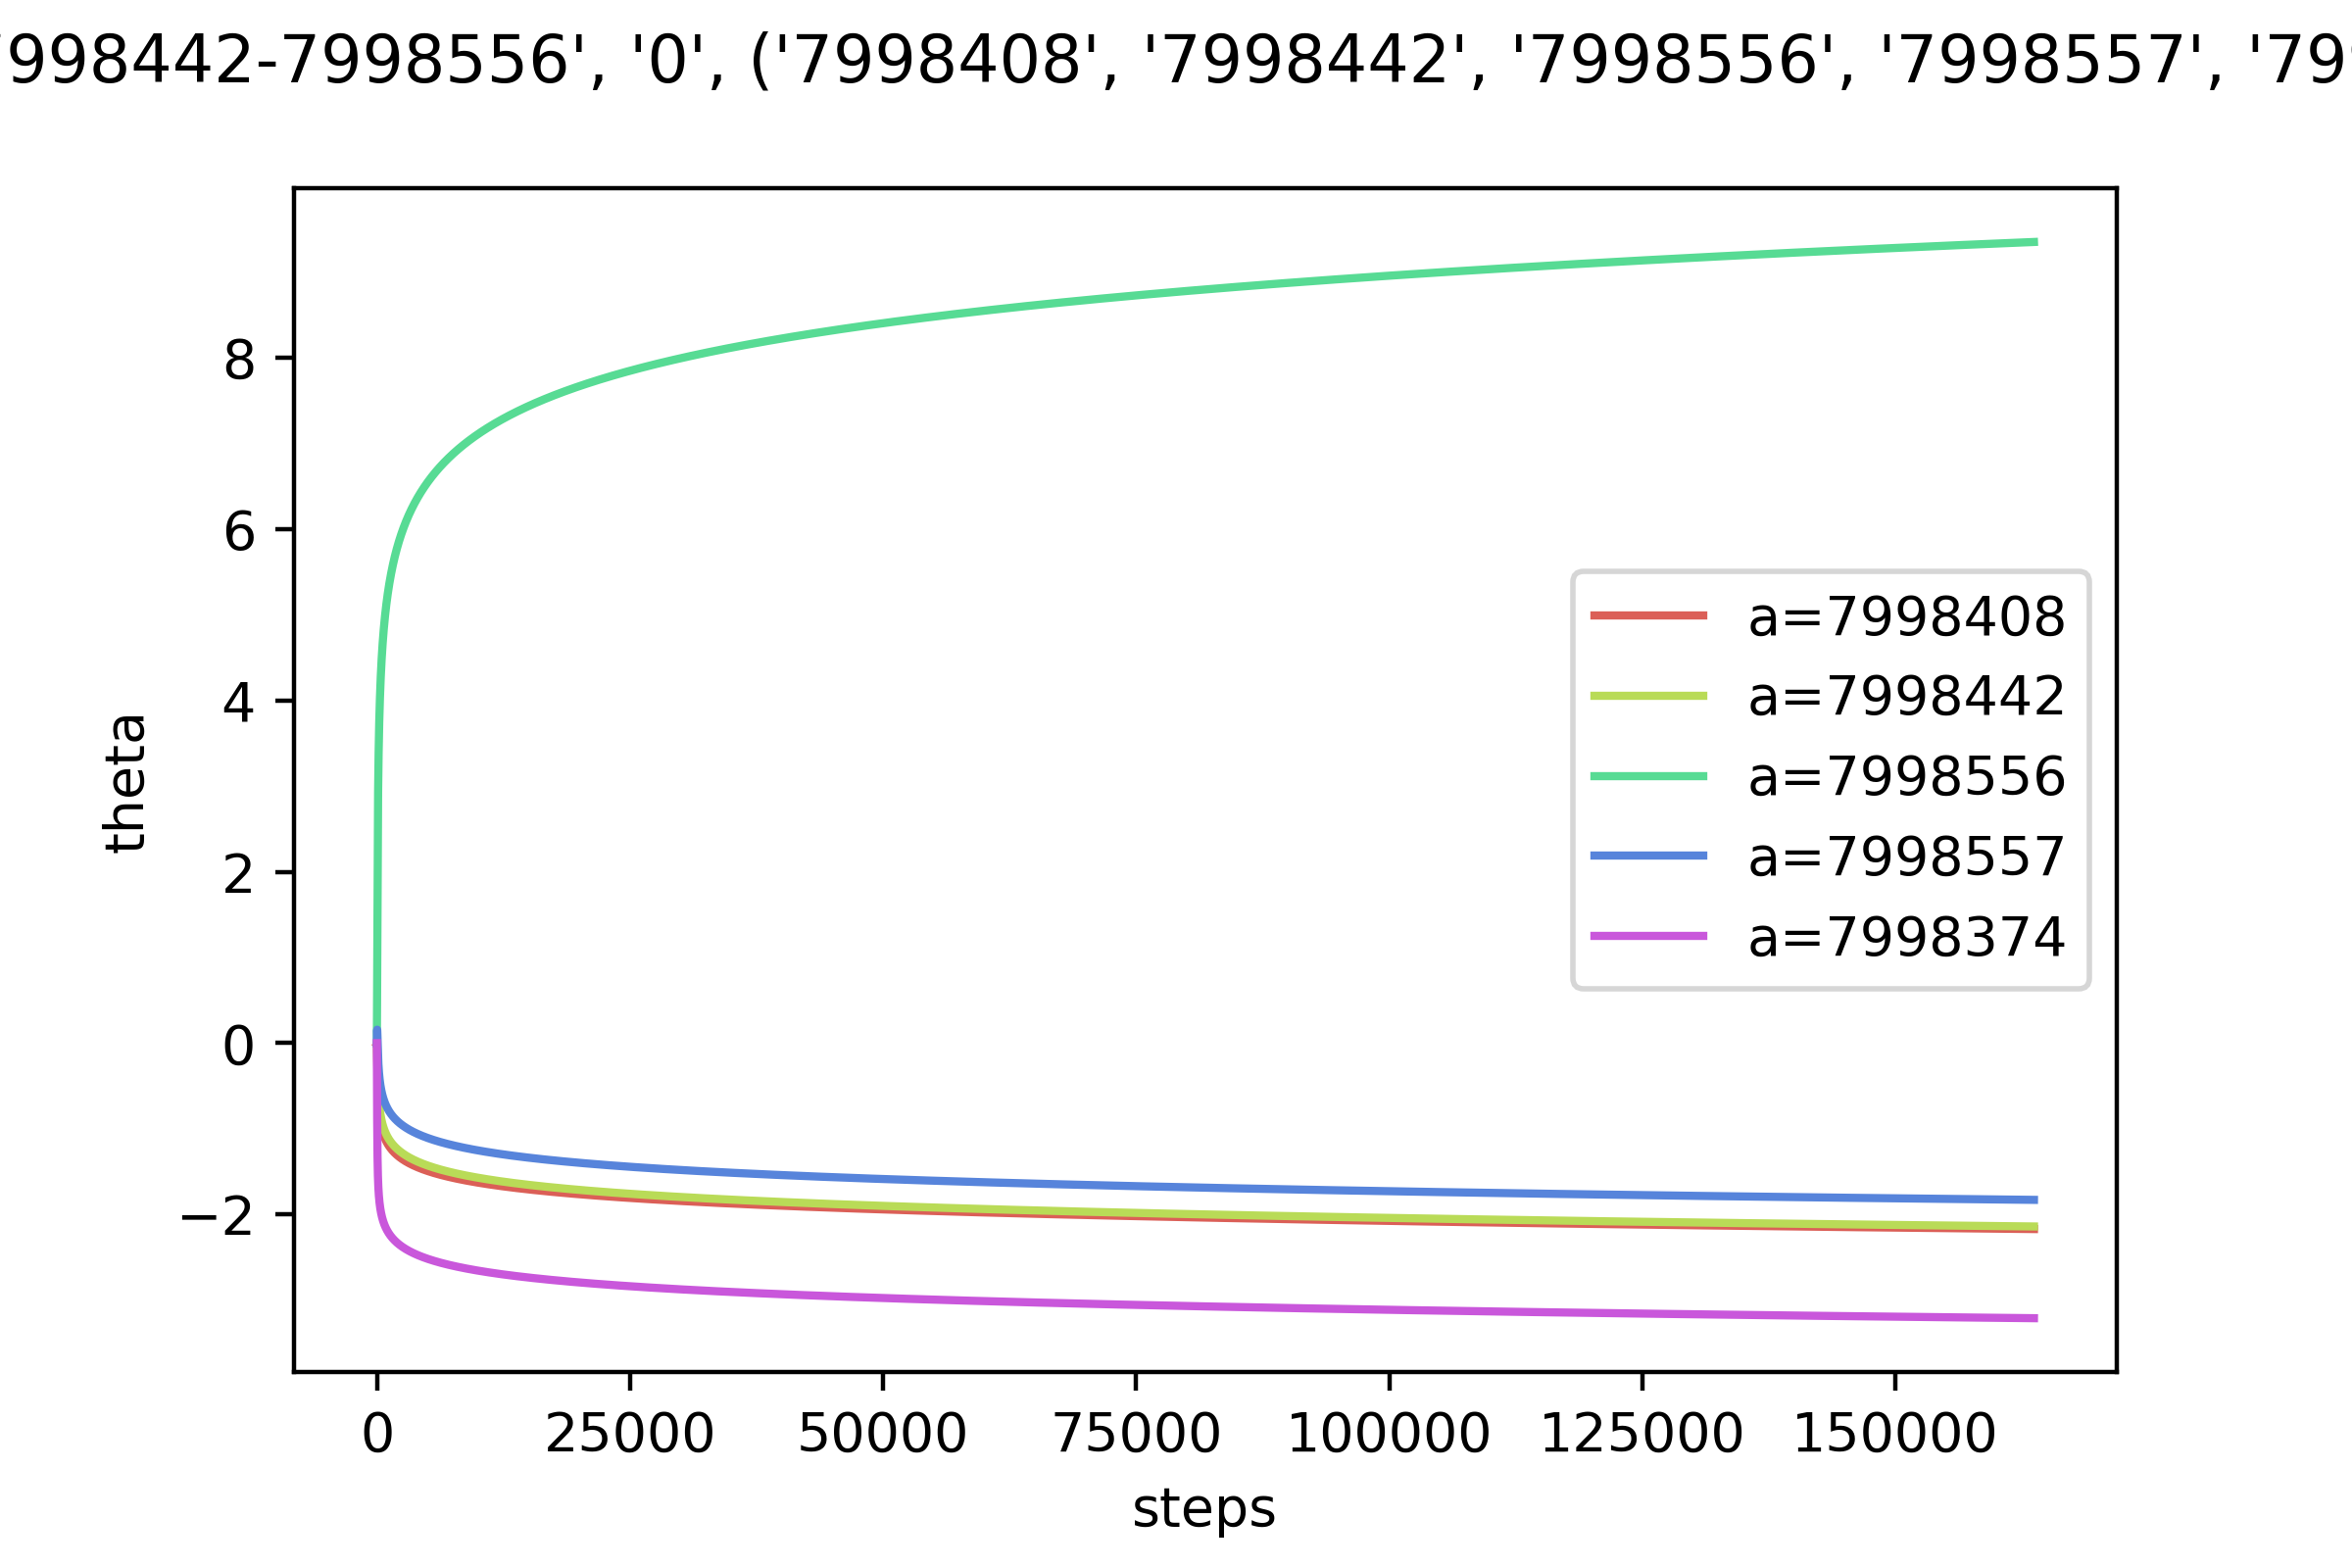
\includegraphics[height=0.27\textwidth,valign=b]{chapters/figures/theta_PG_state_0.png} &
        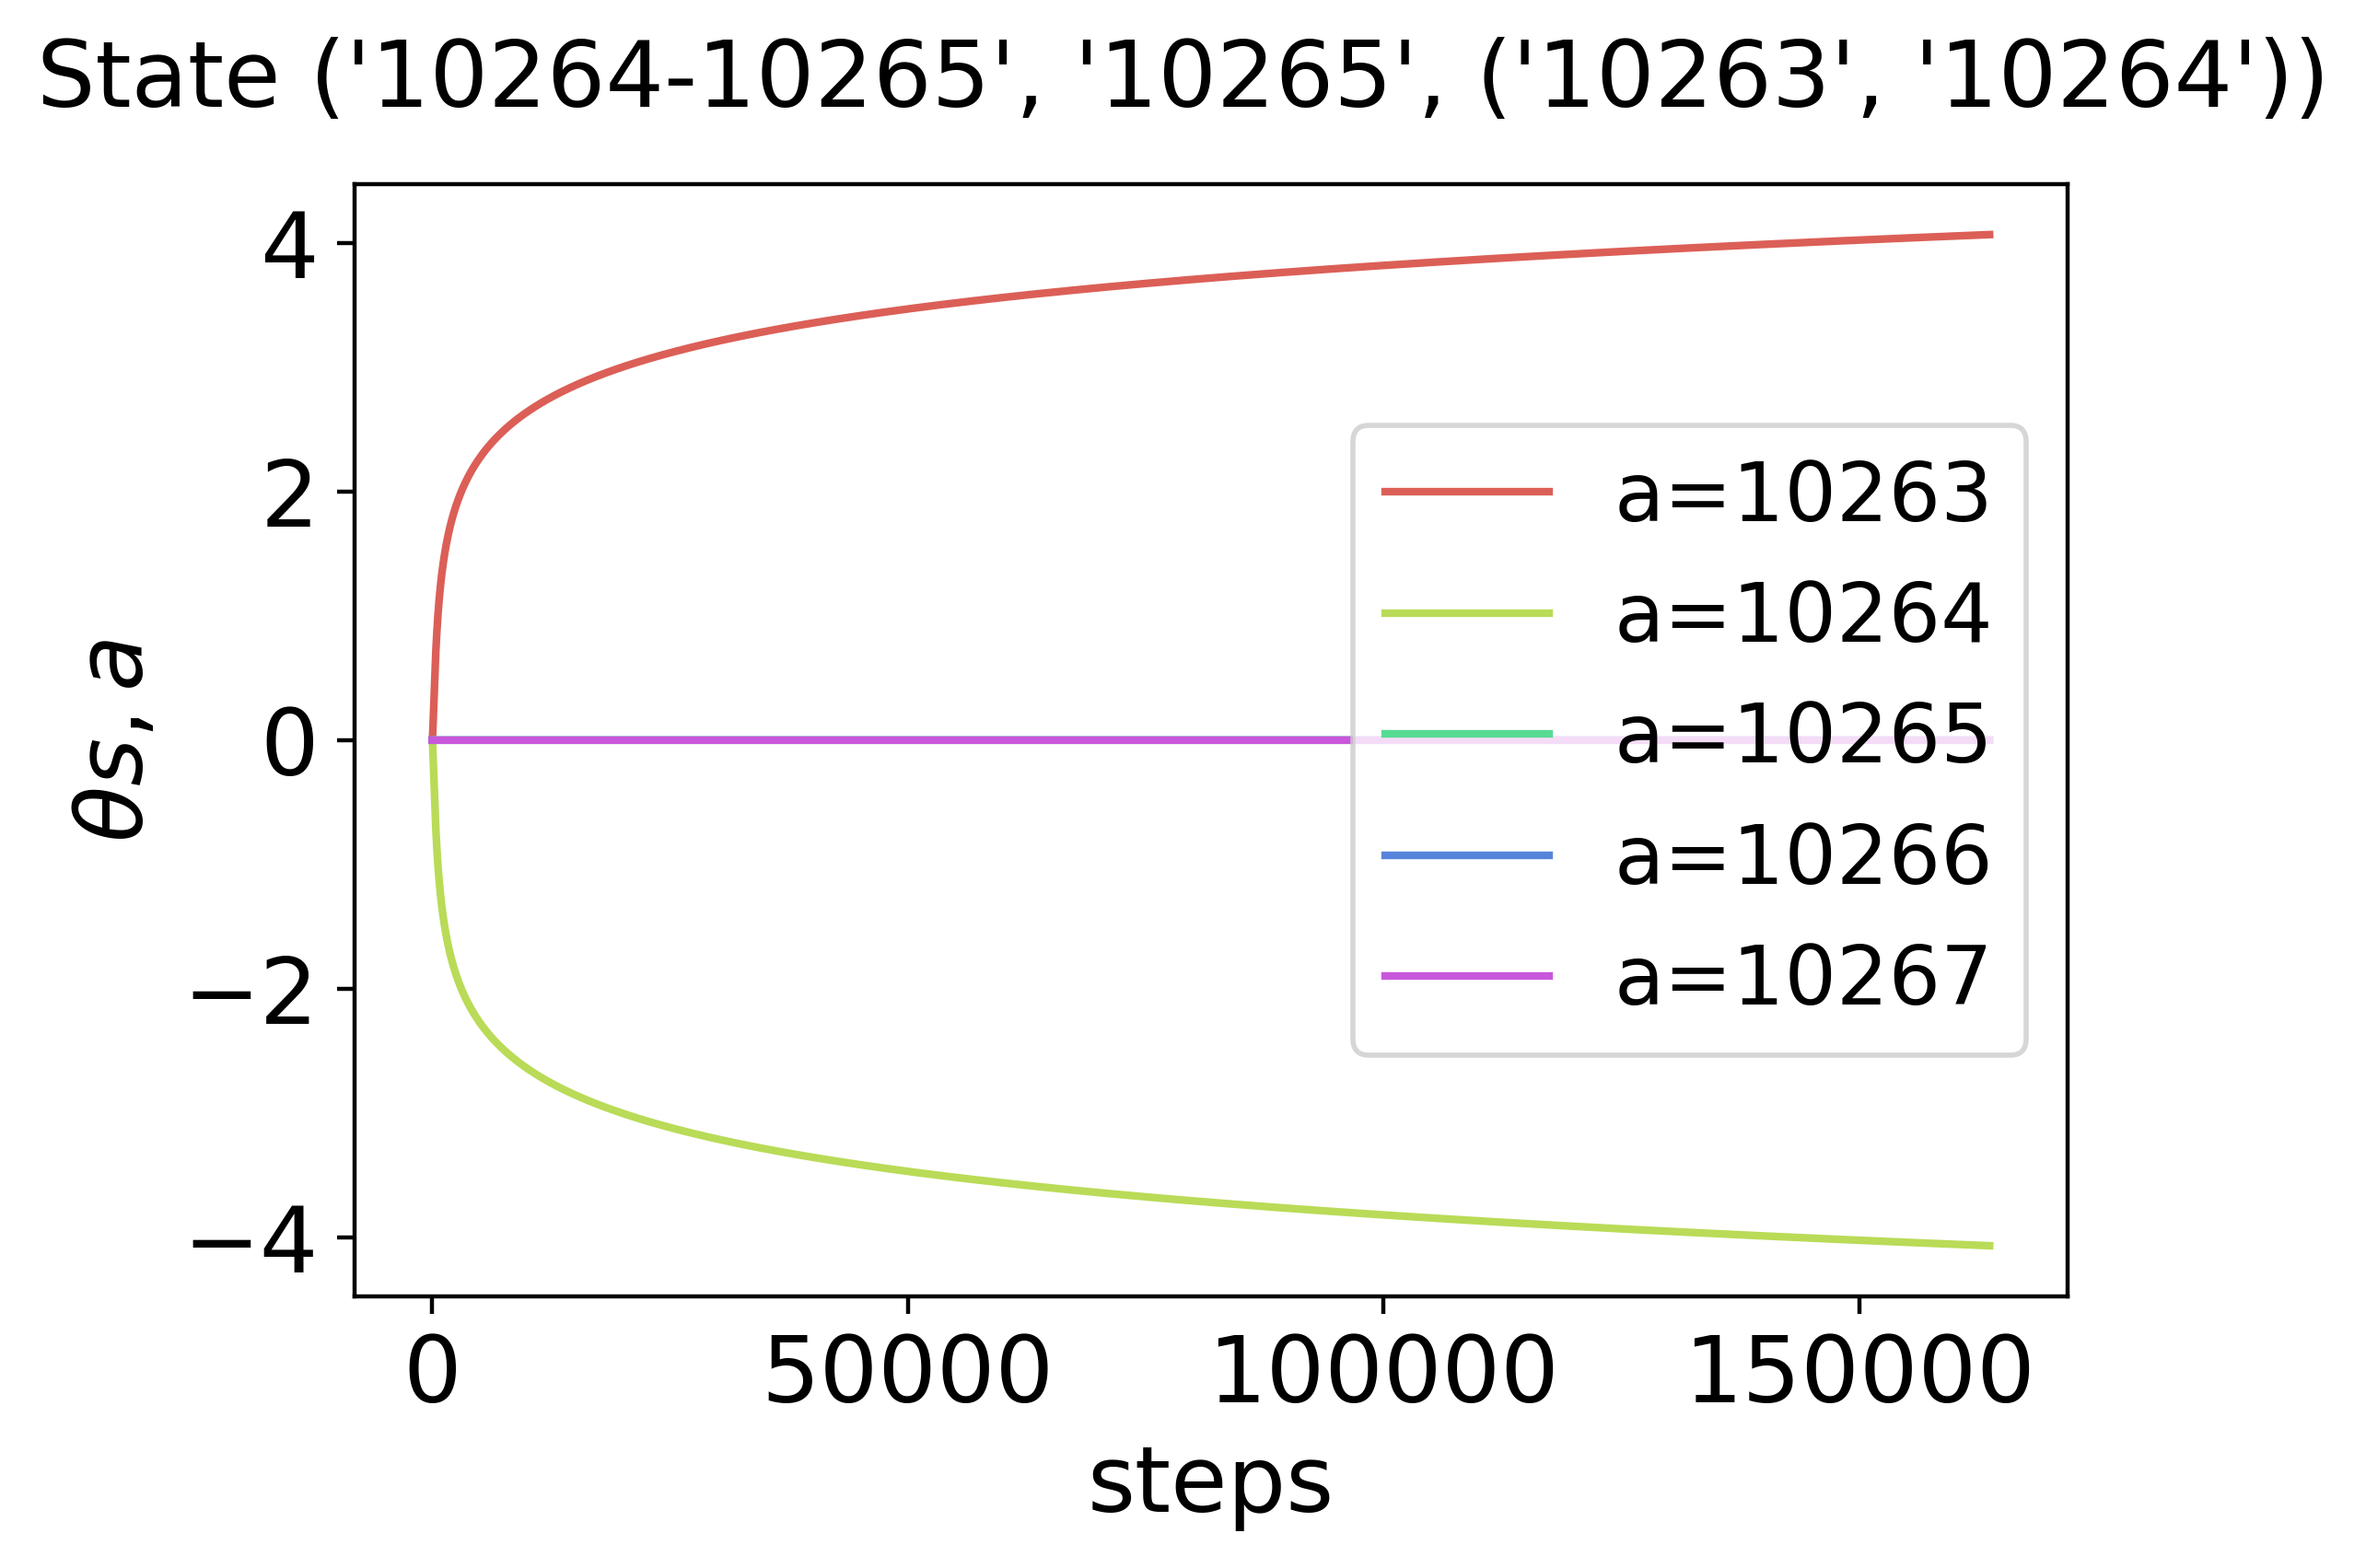
\includegraphics[height=0.27\textwidth,valign=b]{chapters/figures/theta_PG_state_1.png} \\
        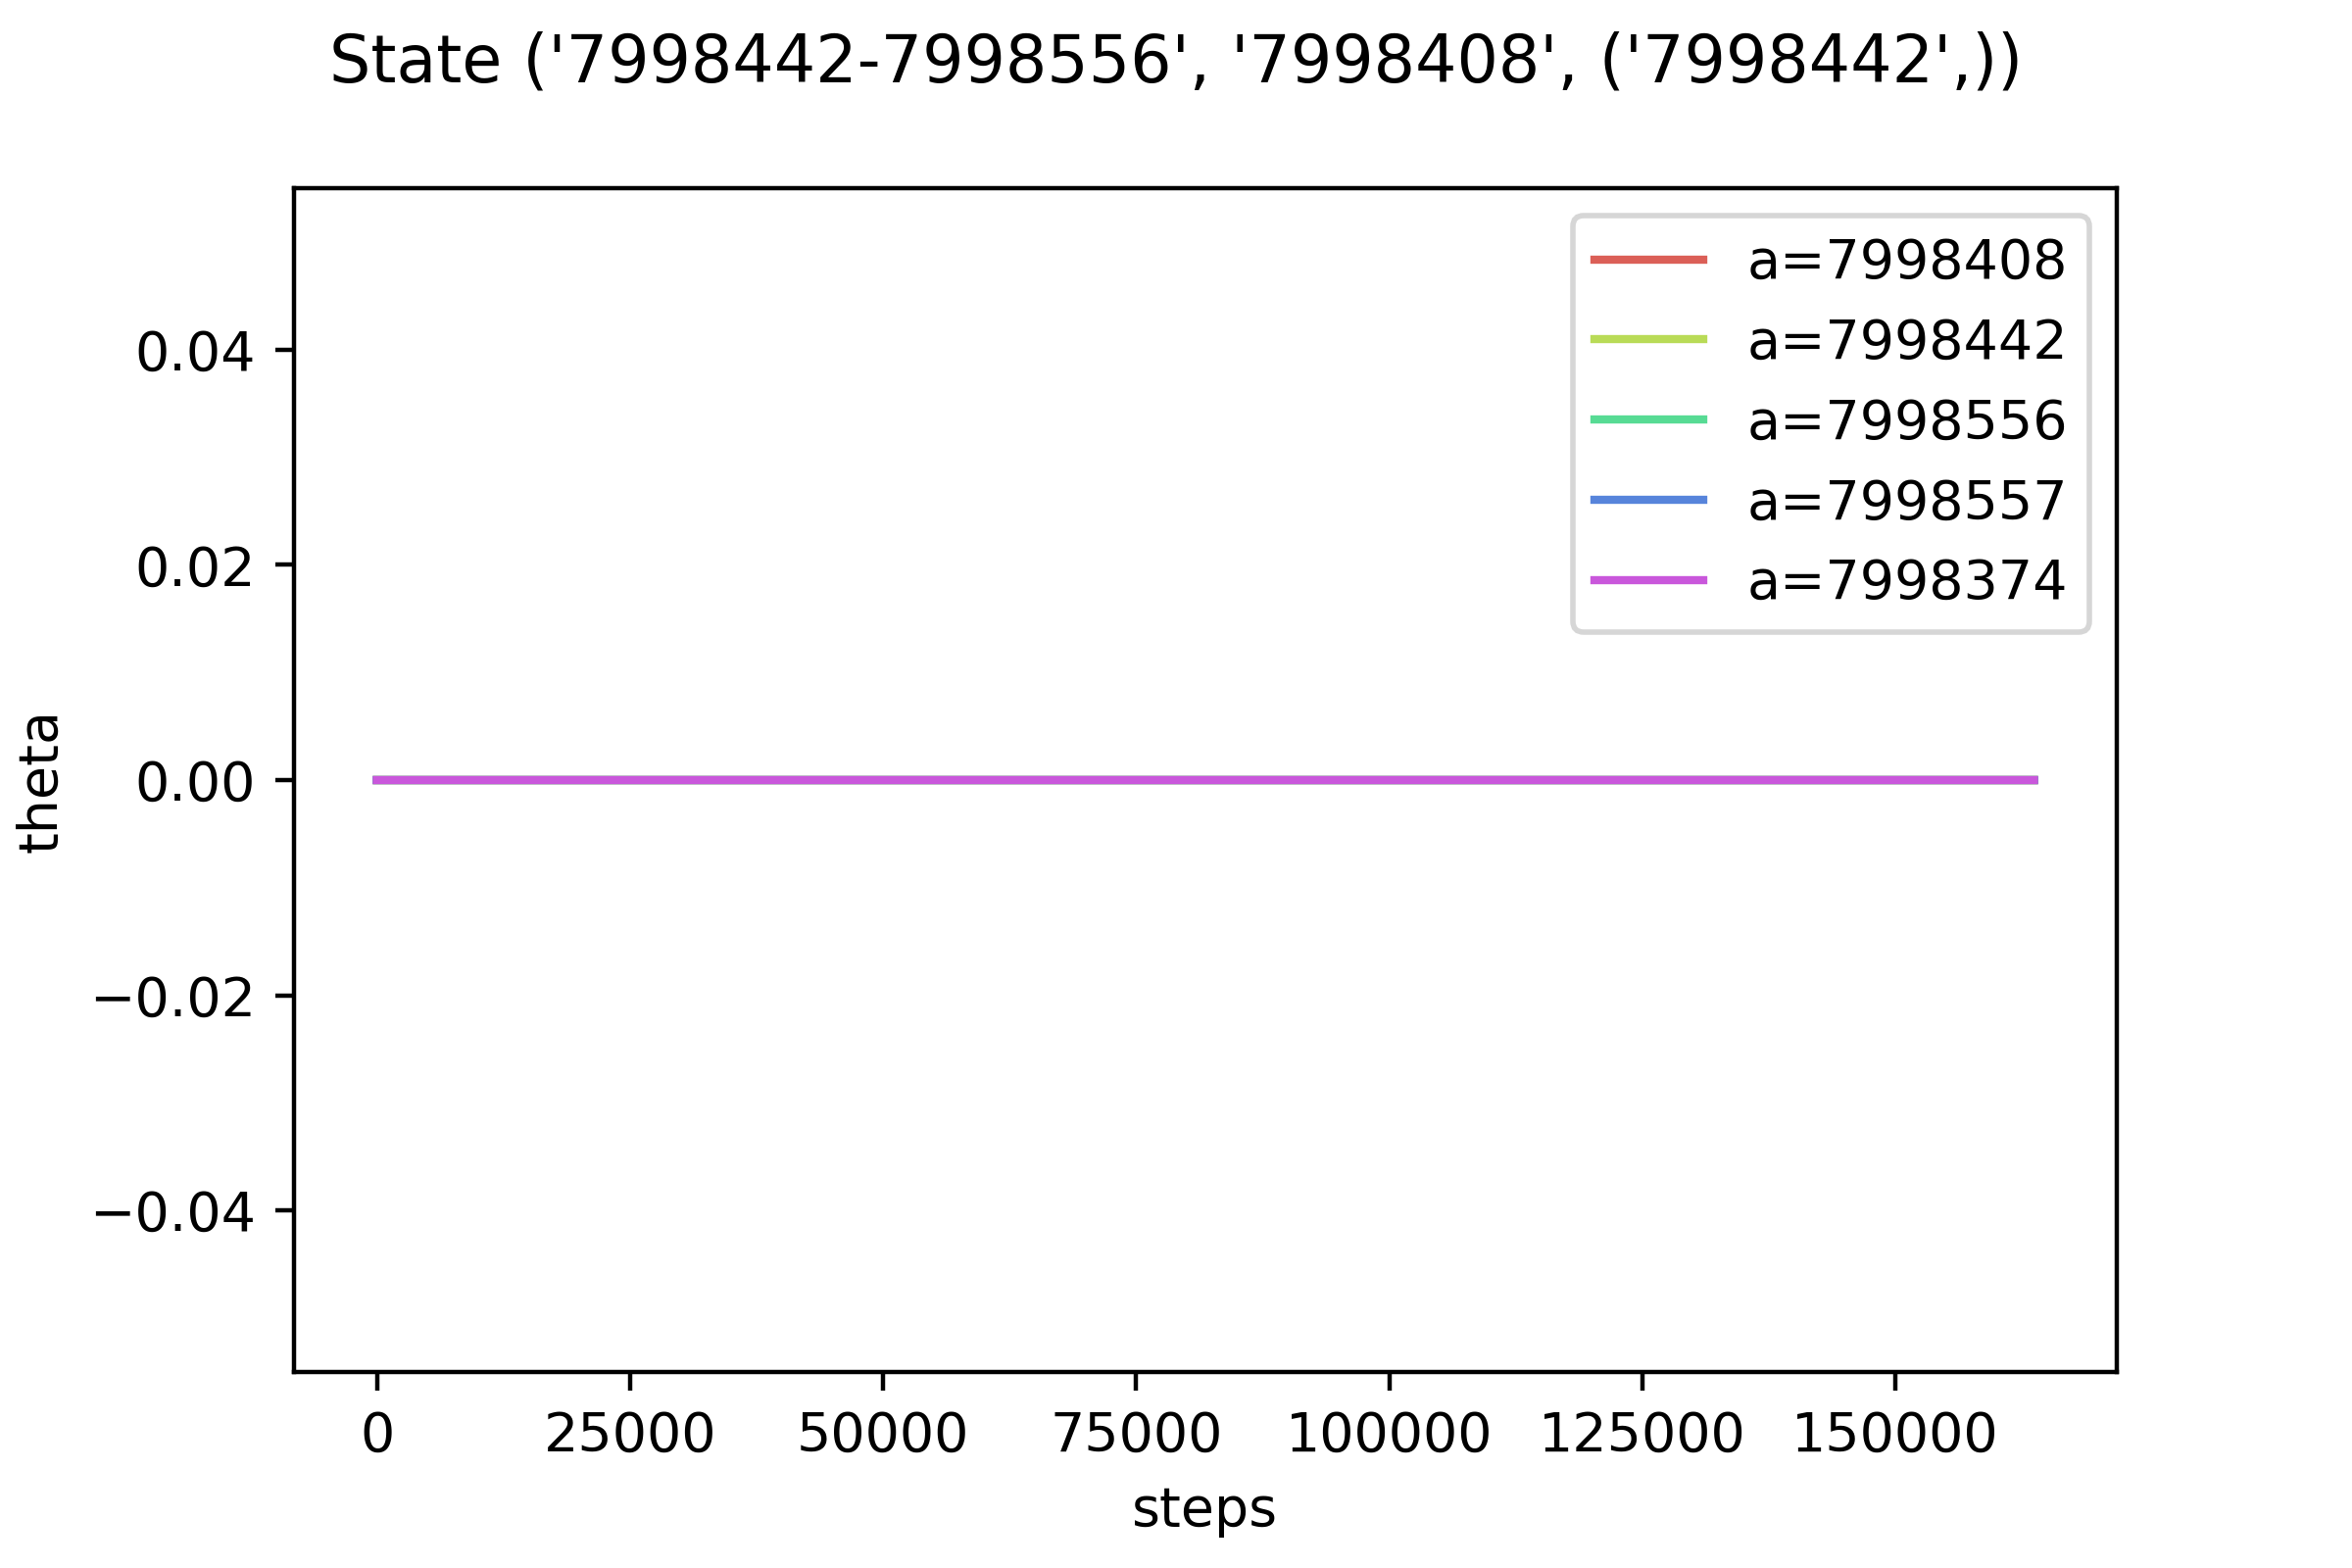
\includegraphics[height=0.27\textwidth,valign=b]{chapters/figures/theta_PG_state_2.png} &
        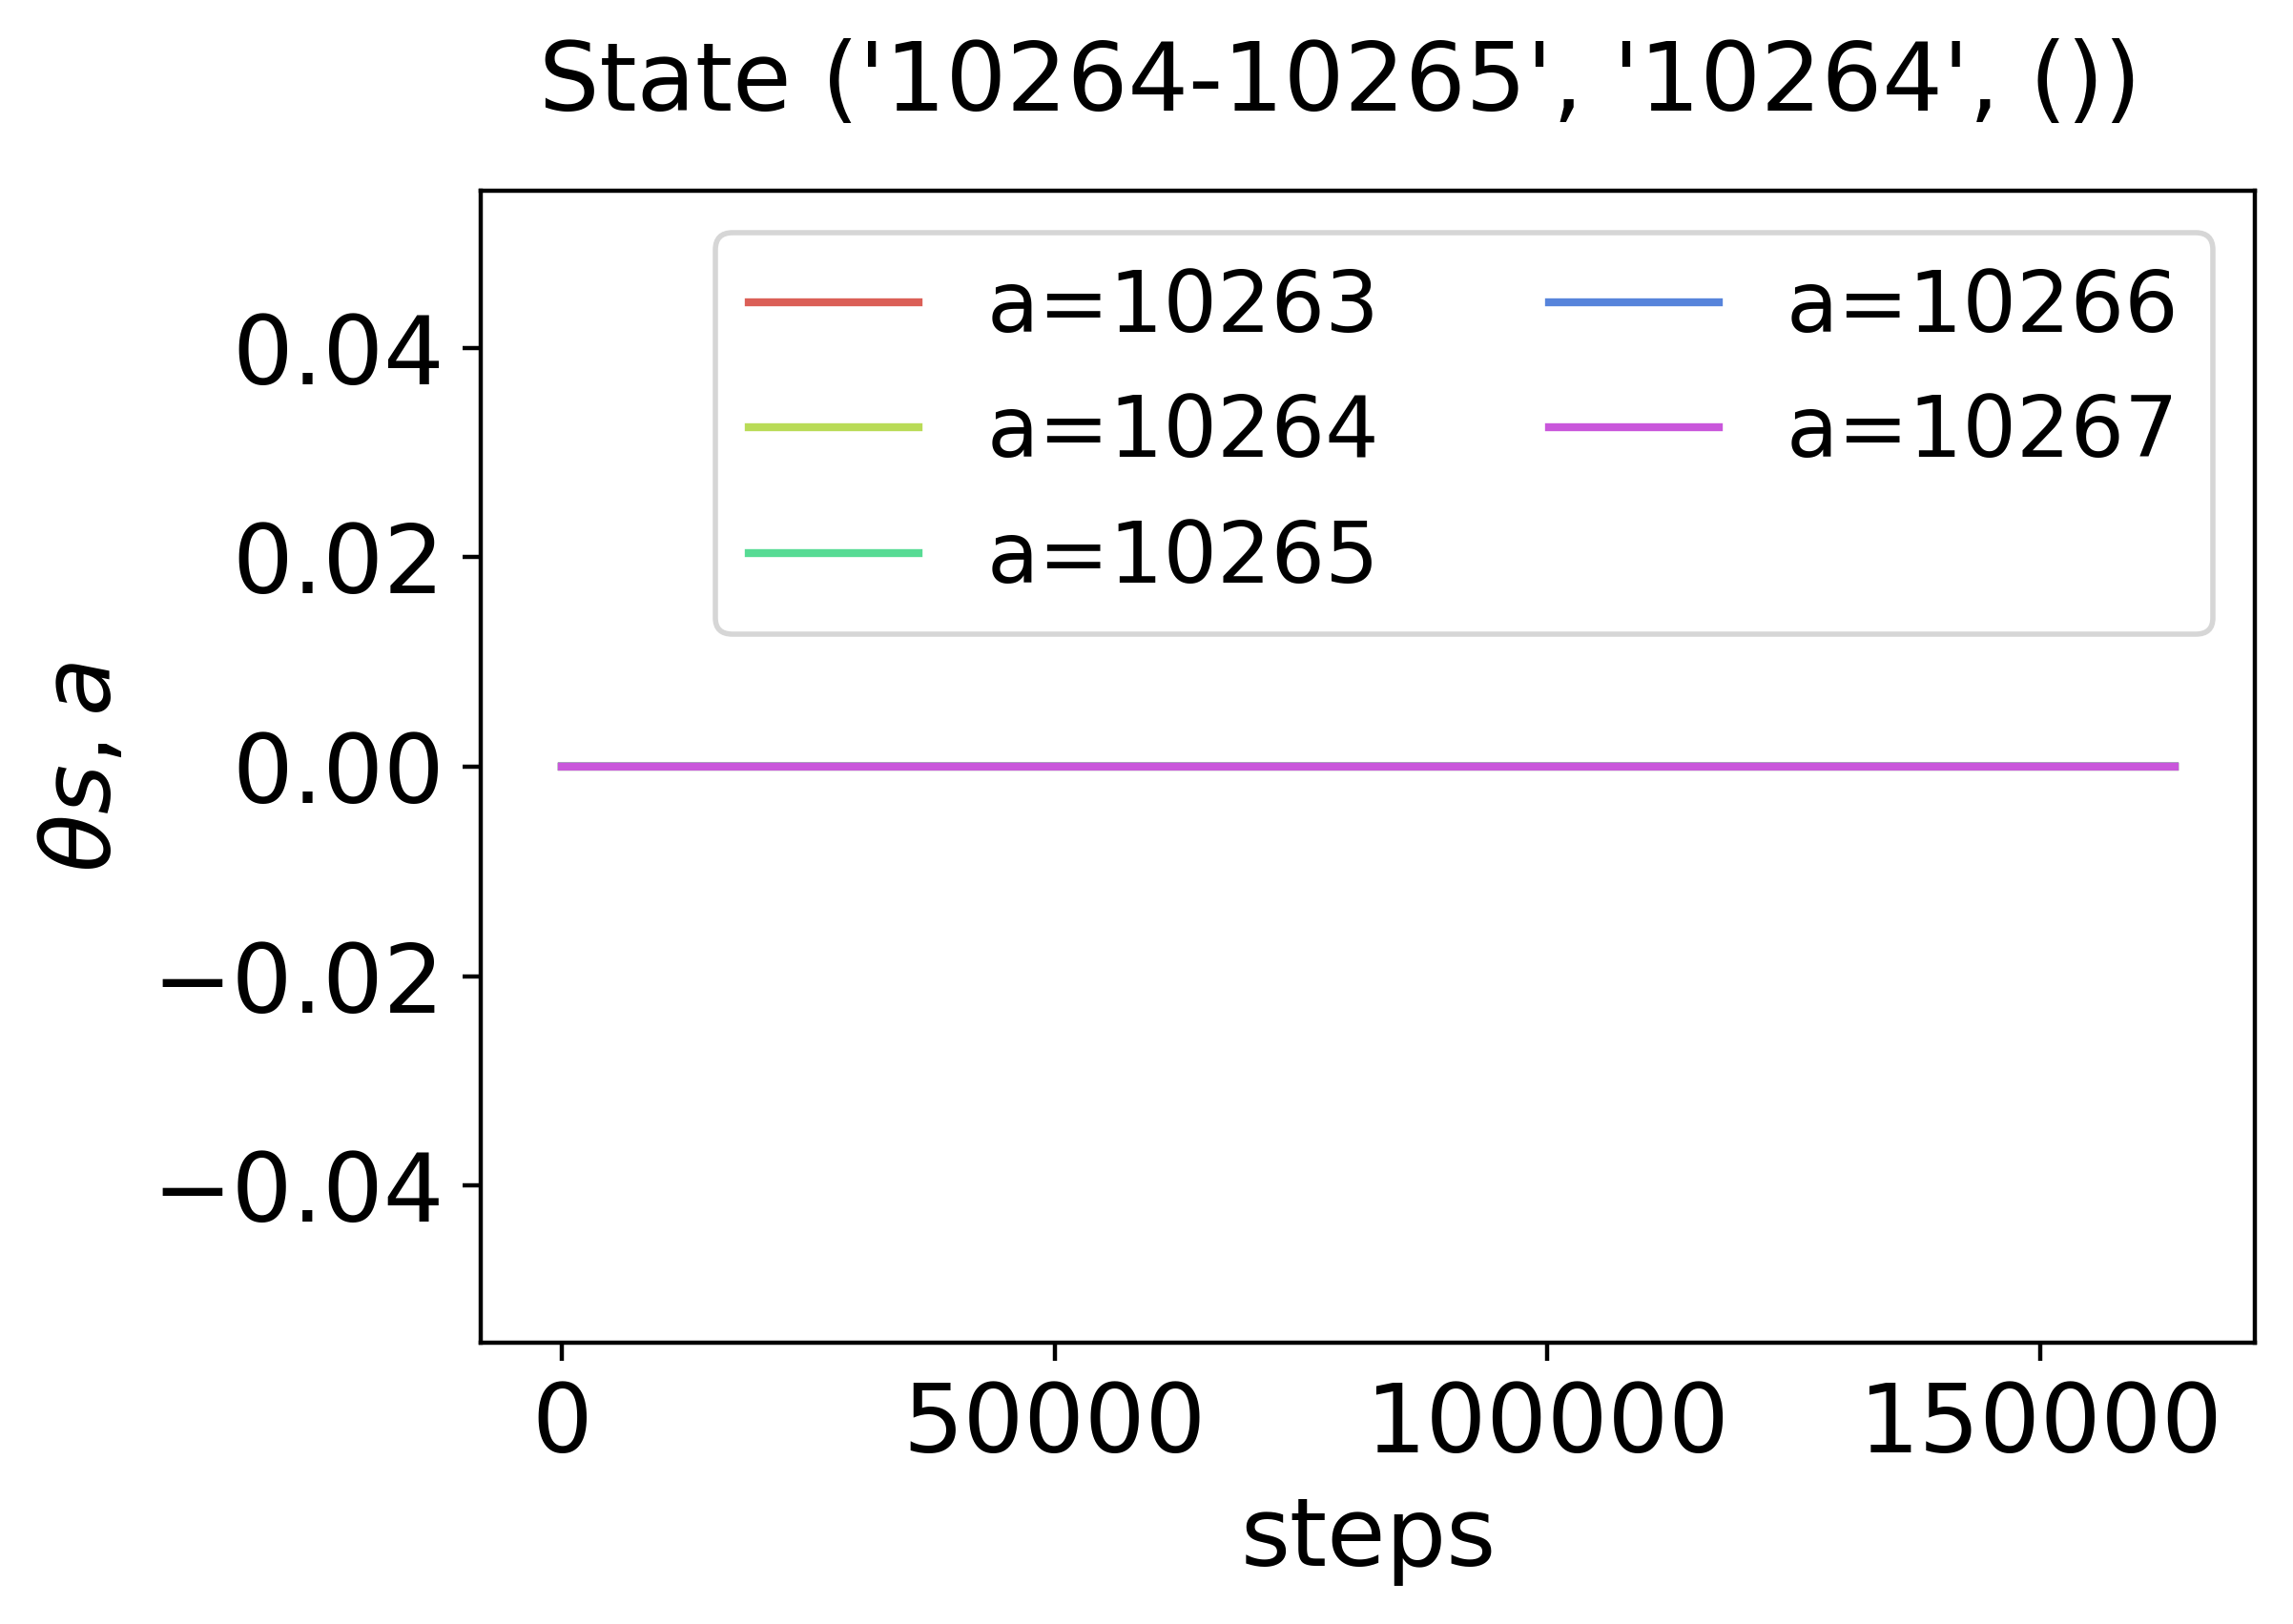
\includegraphics[height=0.27\textwidth,valign=b]{chapters/figures/theta_PG_state_3.png}
    \end{tabular}
    \caption{Trajectories of the parameters $\boldsymbol \theta$ in the parameters space for \acrshort{pg}, for a specific episode with $5$ initially disconnected substation.}
    \label{fig:sequence-theta-pg}
\end{figure}

\begin{figure}[!htp]
    \centering
    \begin{tabular}{cc}
        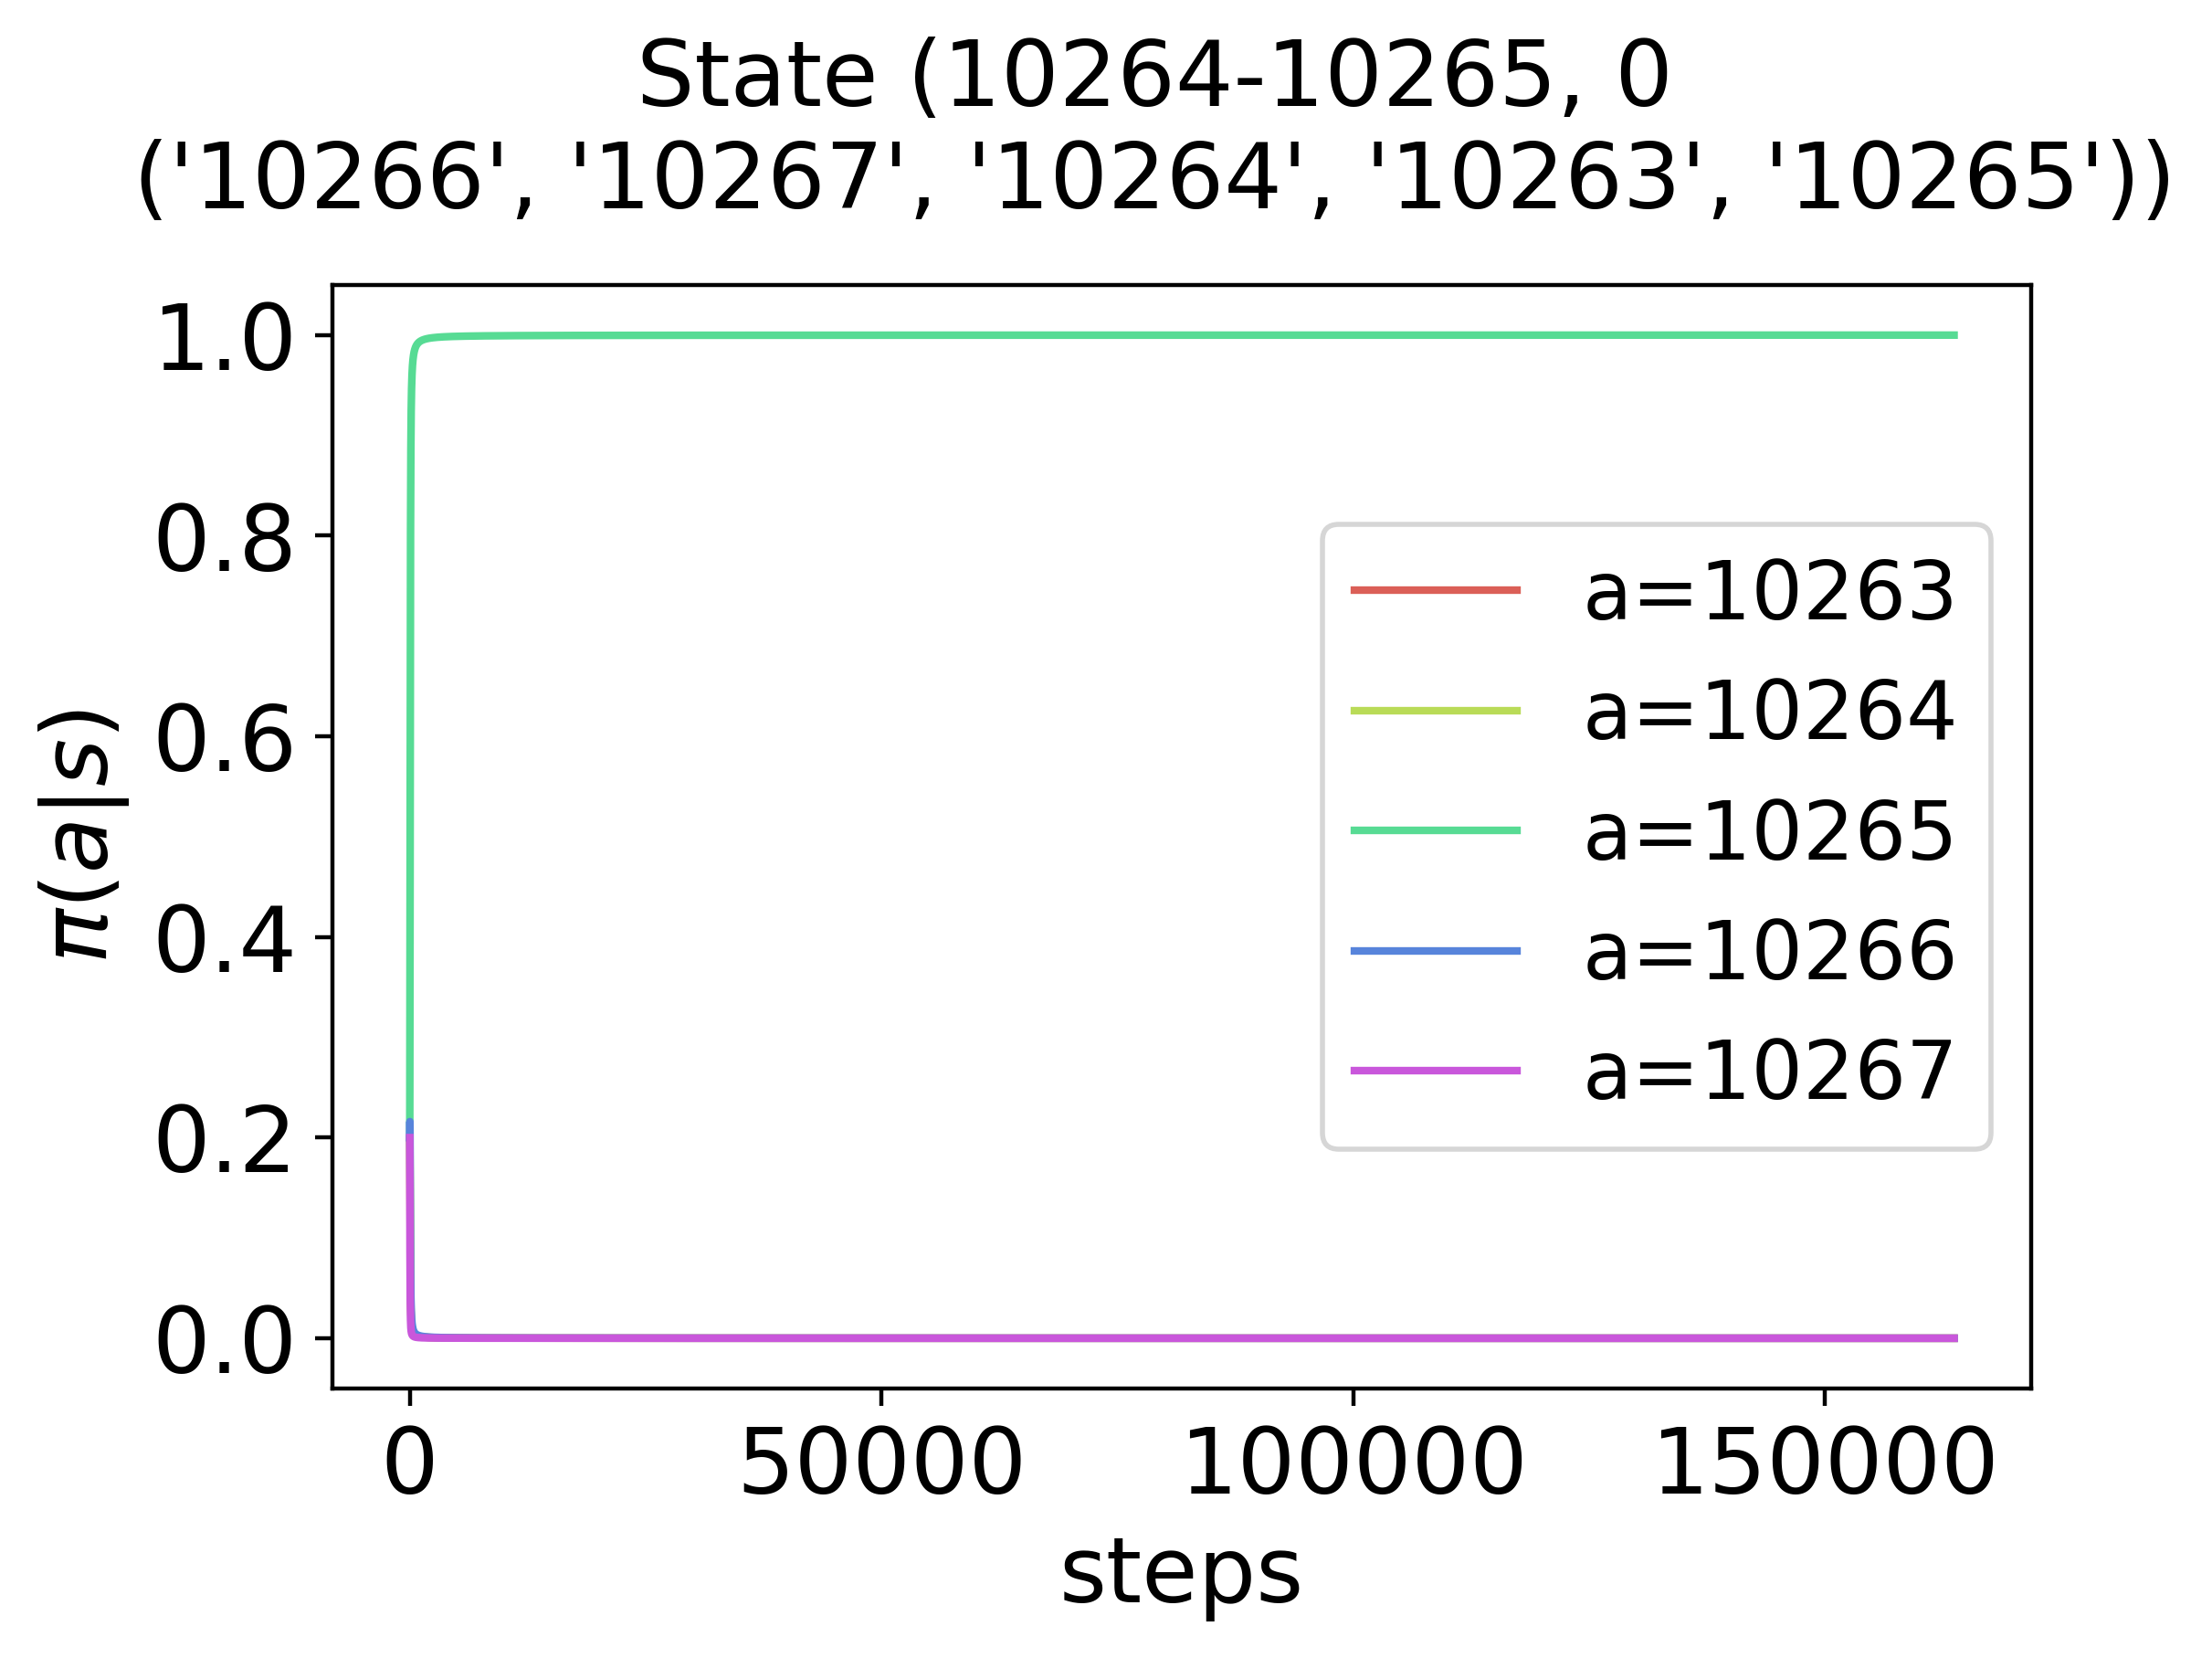
\includegraphics[height=0.27\textwidth,valign=b]{chapters/figures/policy_PG_state_0.png} &
        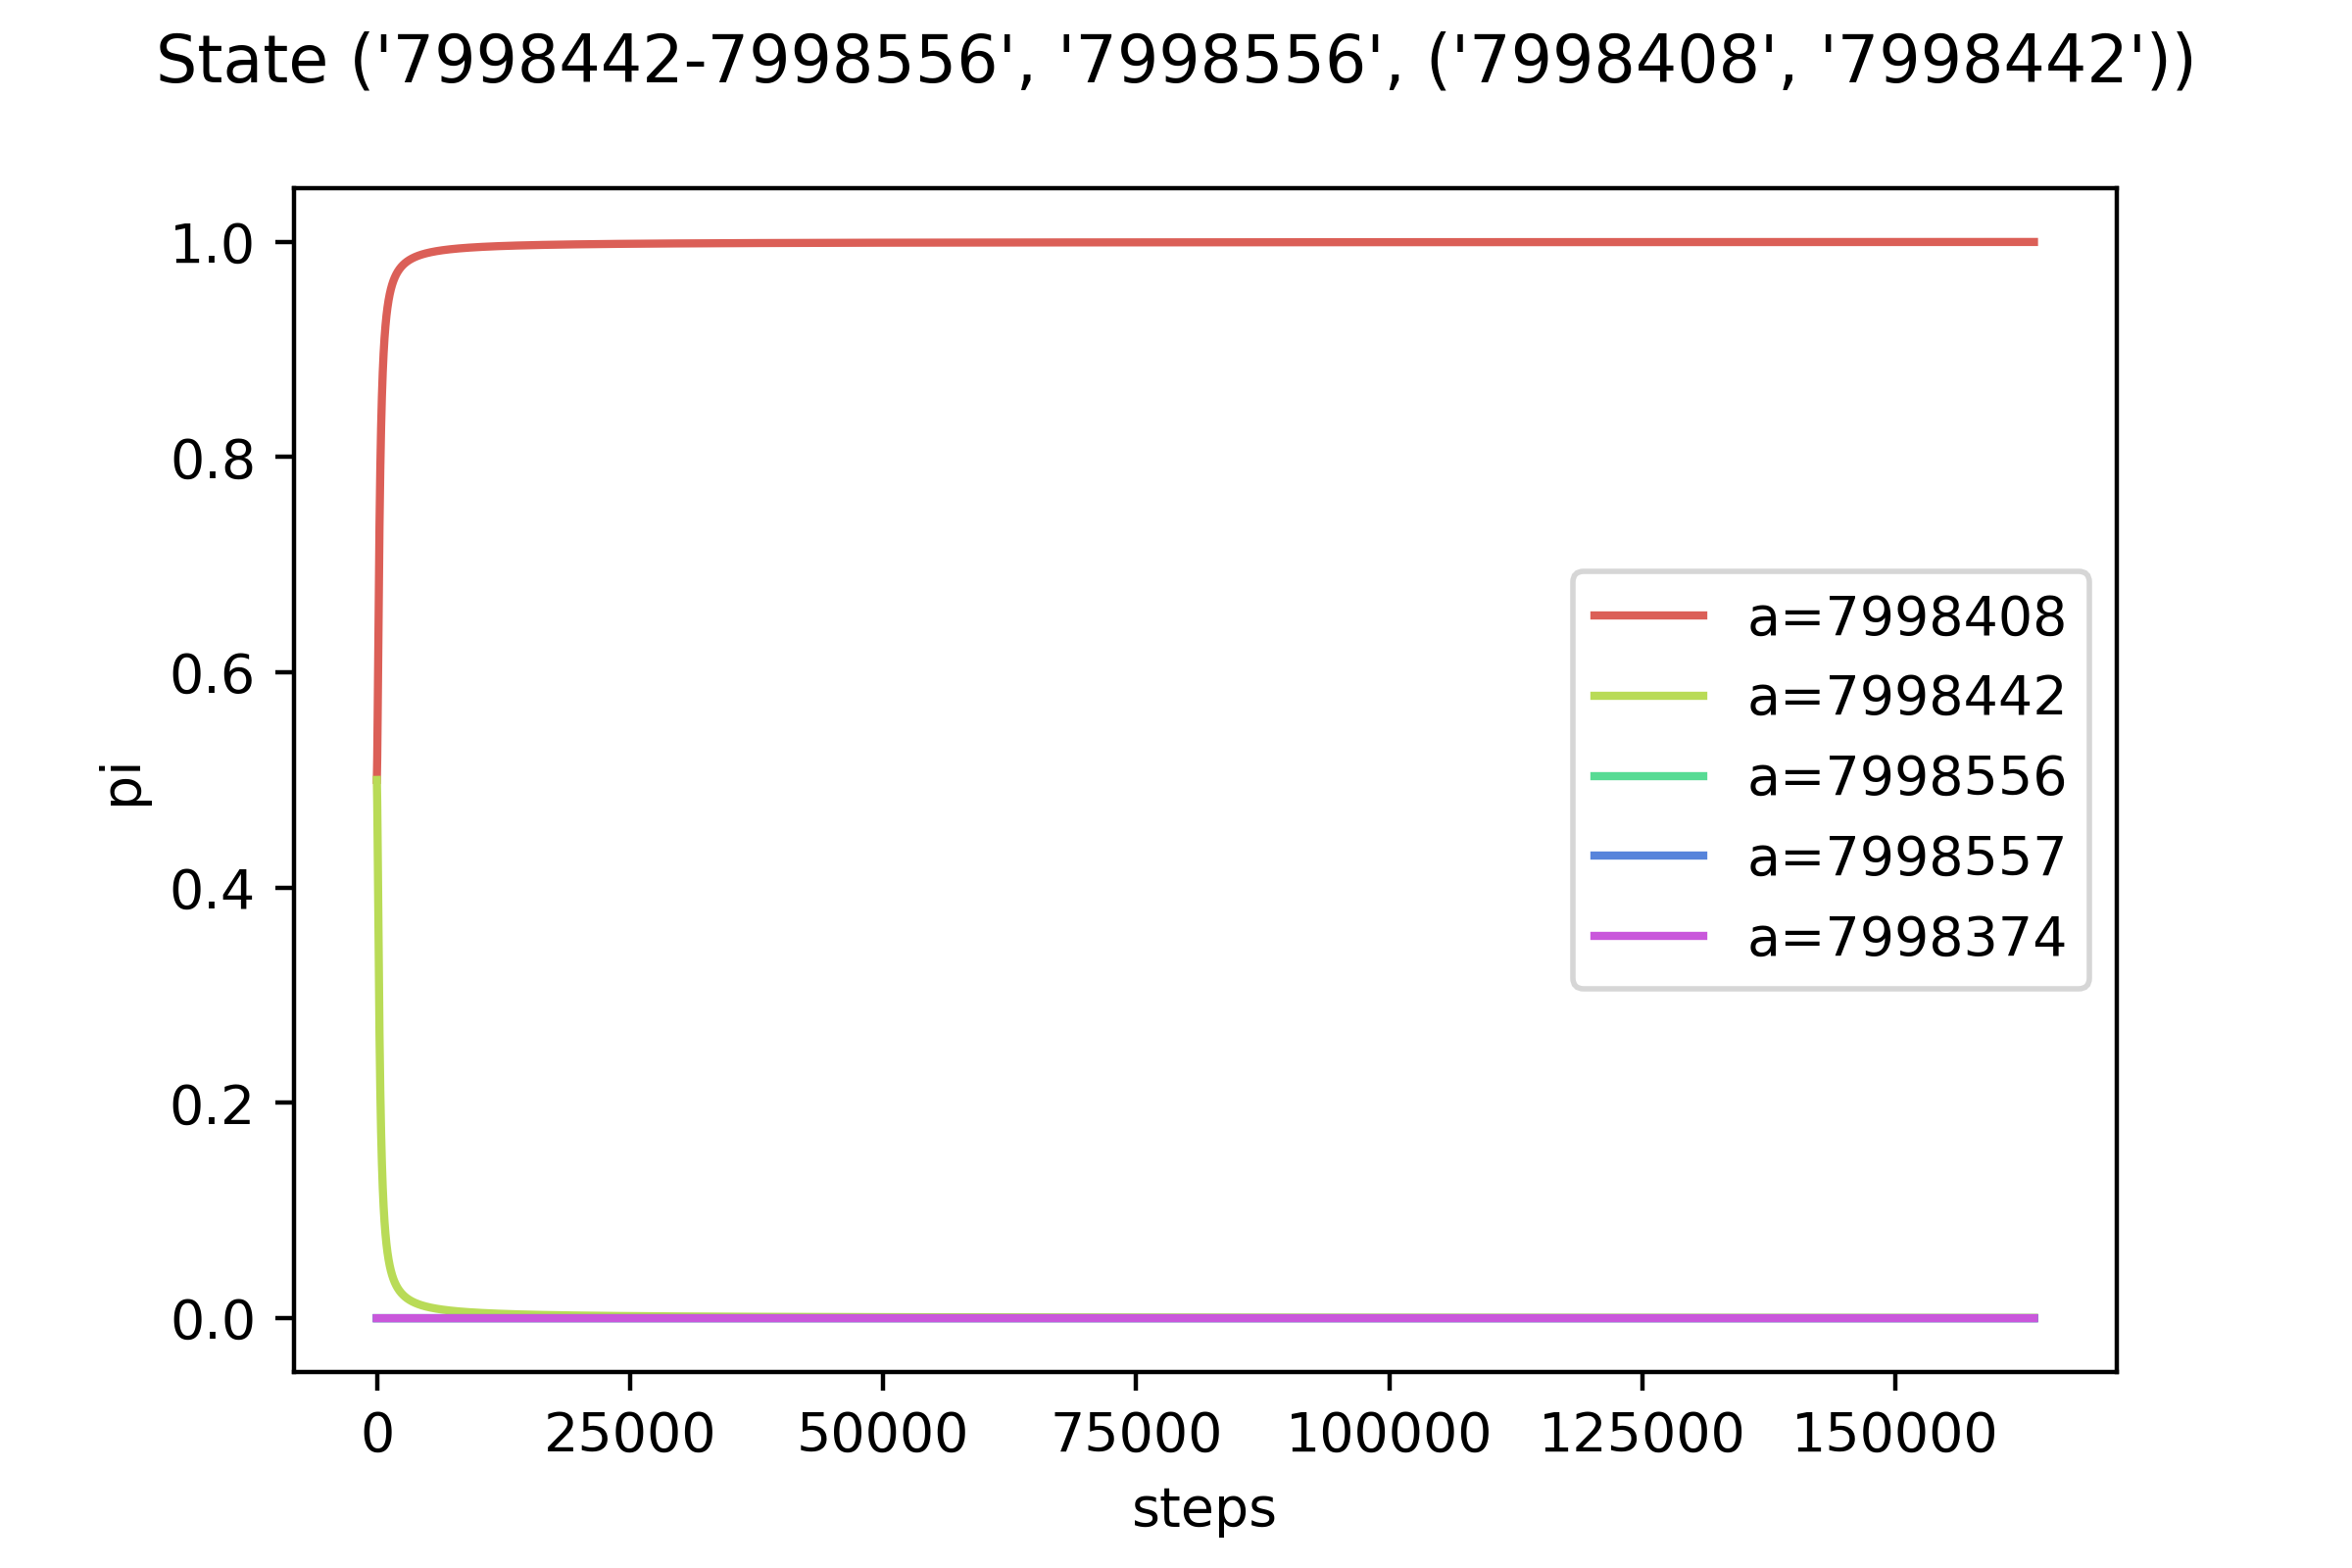
\includegraphics[height=0.27\textwidth,valign=b]{chapters/figures/policy_PG_state_1.png} \\
        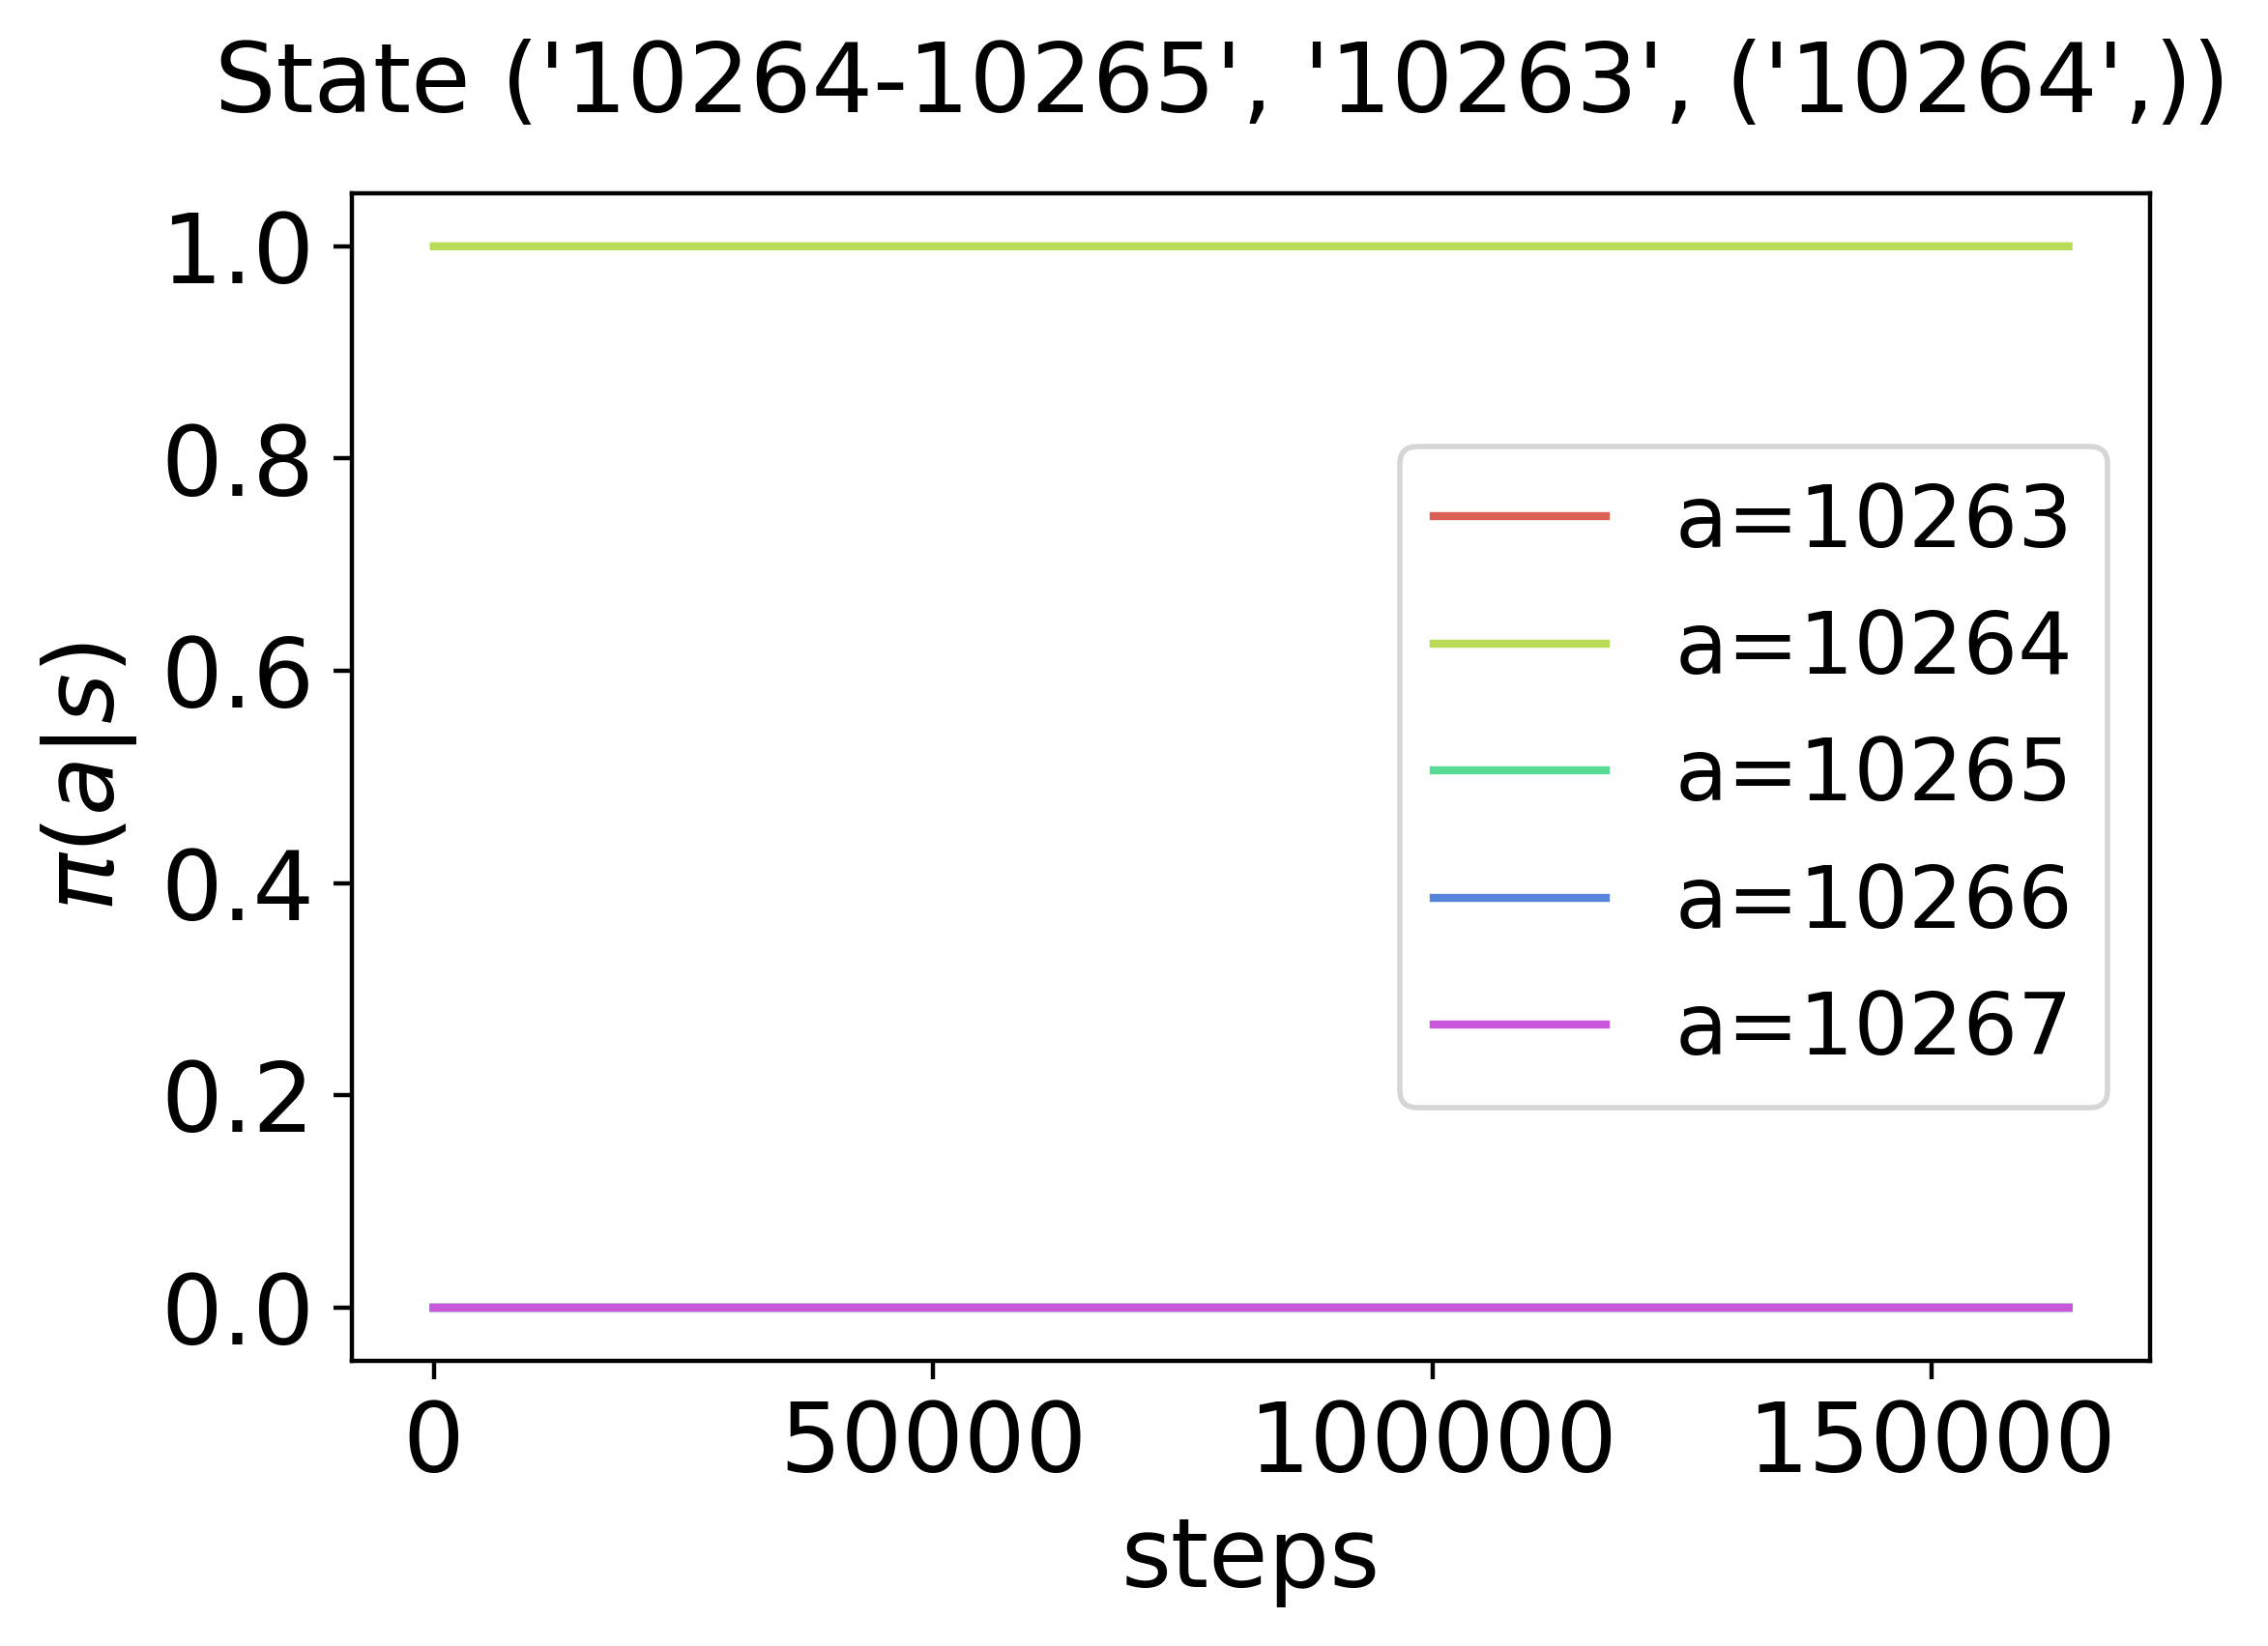
\includegraphics[height=0.27\textwidth,valign=b]{chapters/figures/policy_PG_state_2.png} &
        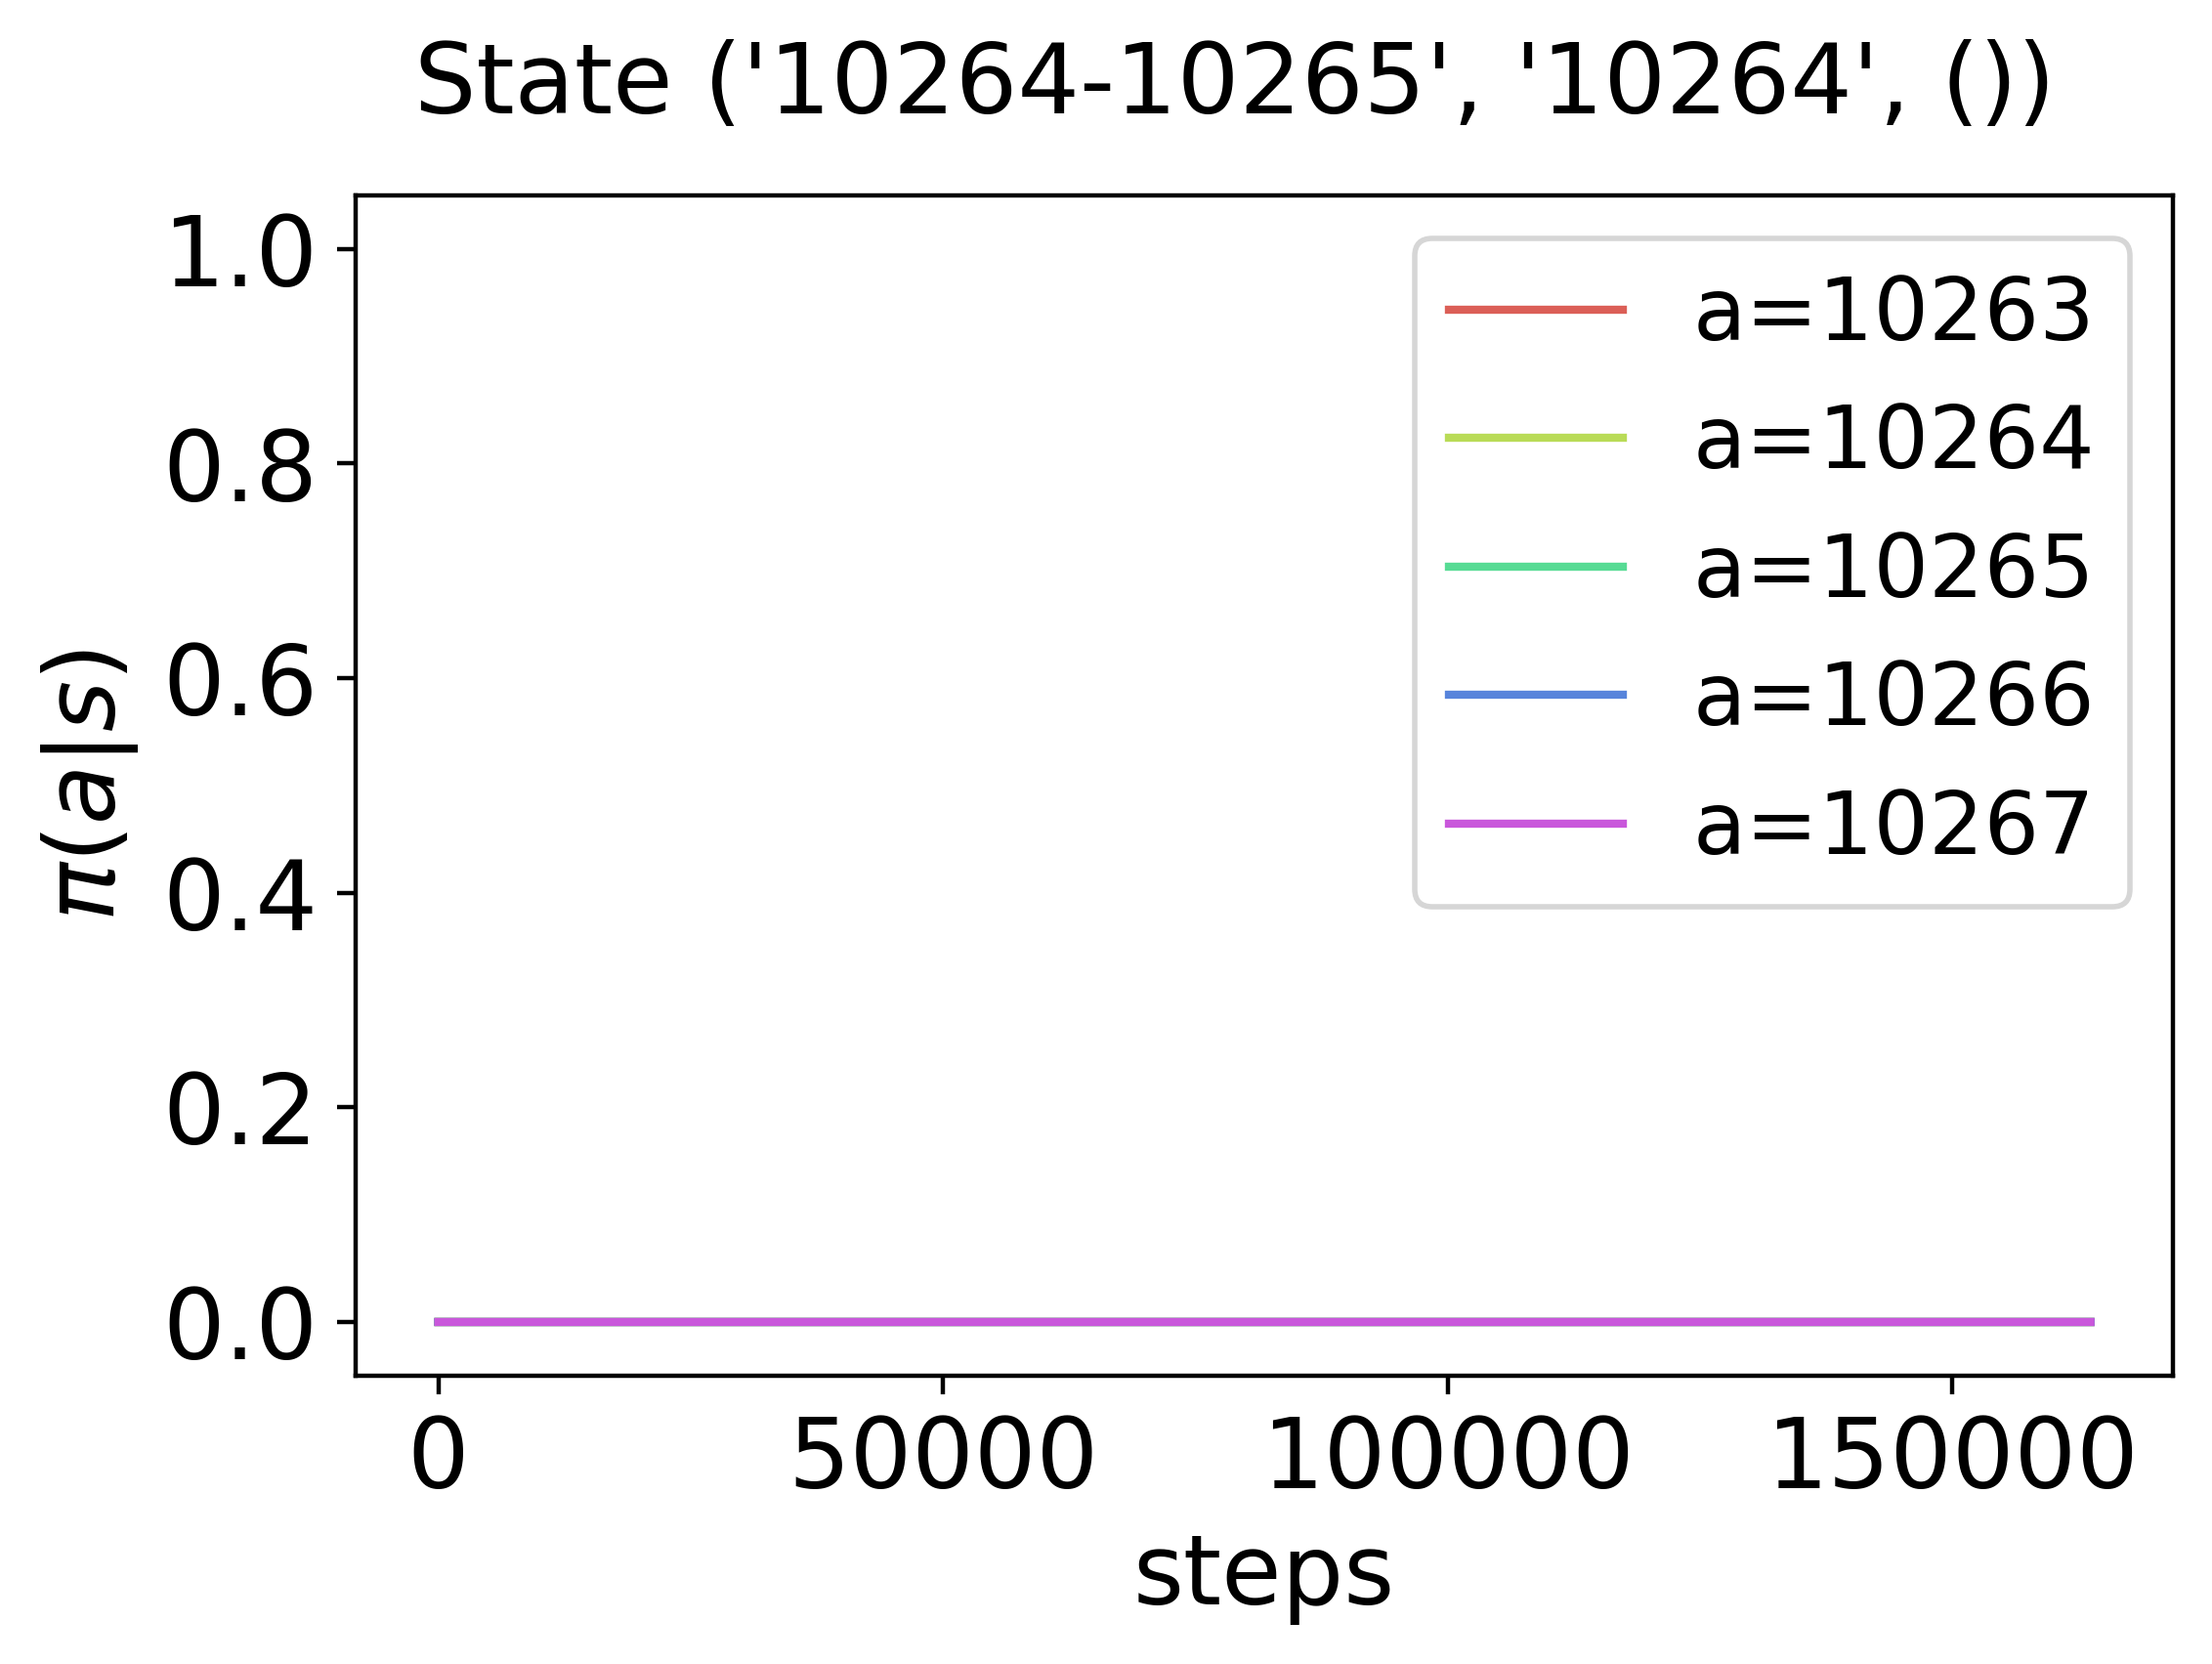
\includegraphics[height=0.27\textwidth,valign=b]{chapters/figures/policy_PG_state_3.png}
    \end{tabular}
    \caption{Trajectories of the policies $\pi_{\boldsymbol \theta}$ in the policy space for \acrshort{pg}, for a specific episode with $5$ initially disconnected substation.}
    \label{fig:sequence-policies-pg}
\end{figure}

\begin{figure}[!htp]
    \centering
    \begin{tabular}{cc}
        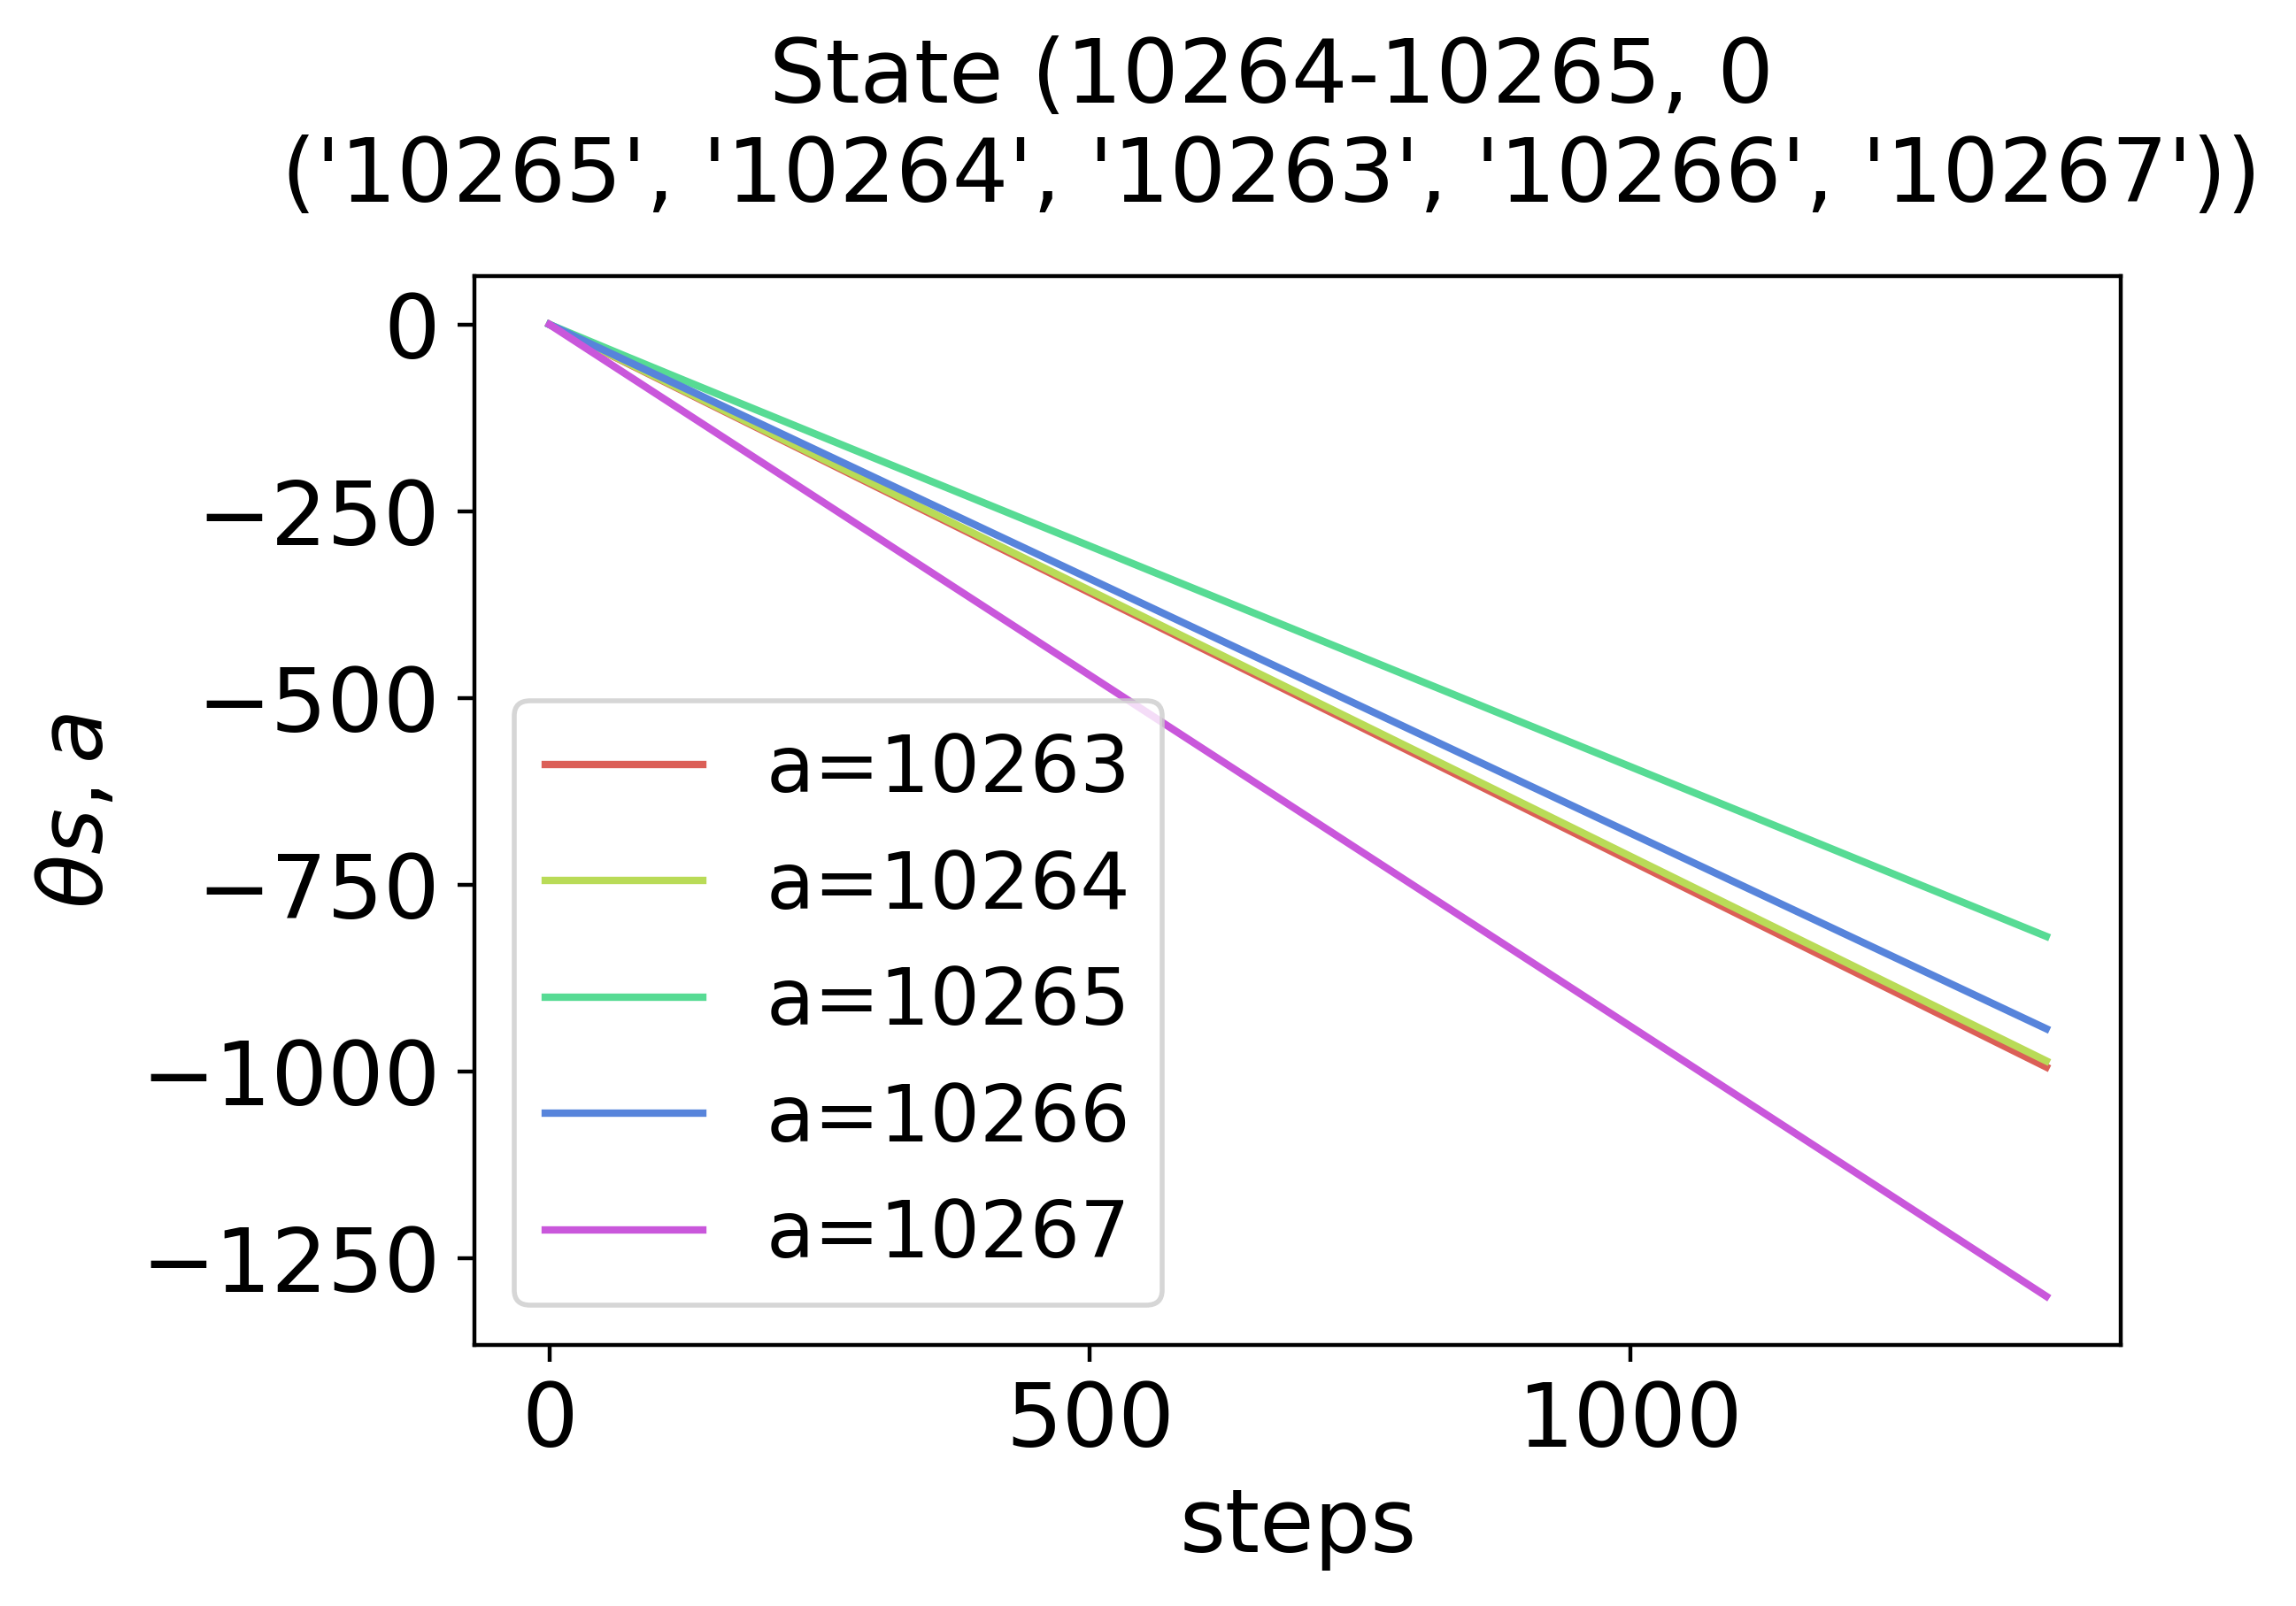
\includegraphics[height=0.27\textwidth,valign=b]{chapters/figures/theta_NPG_state_0.png} &
        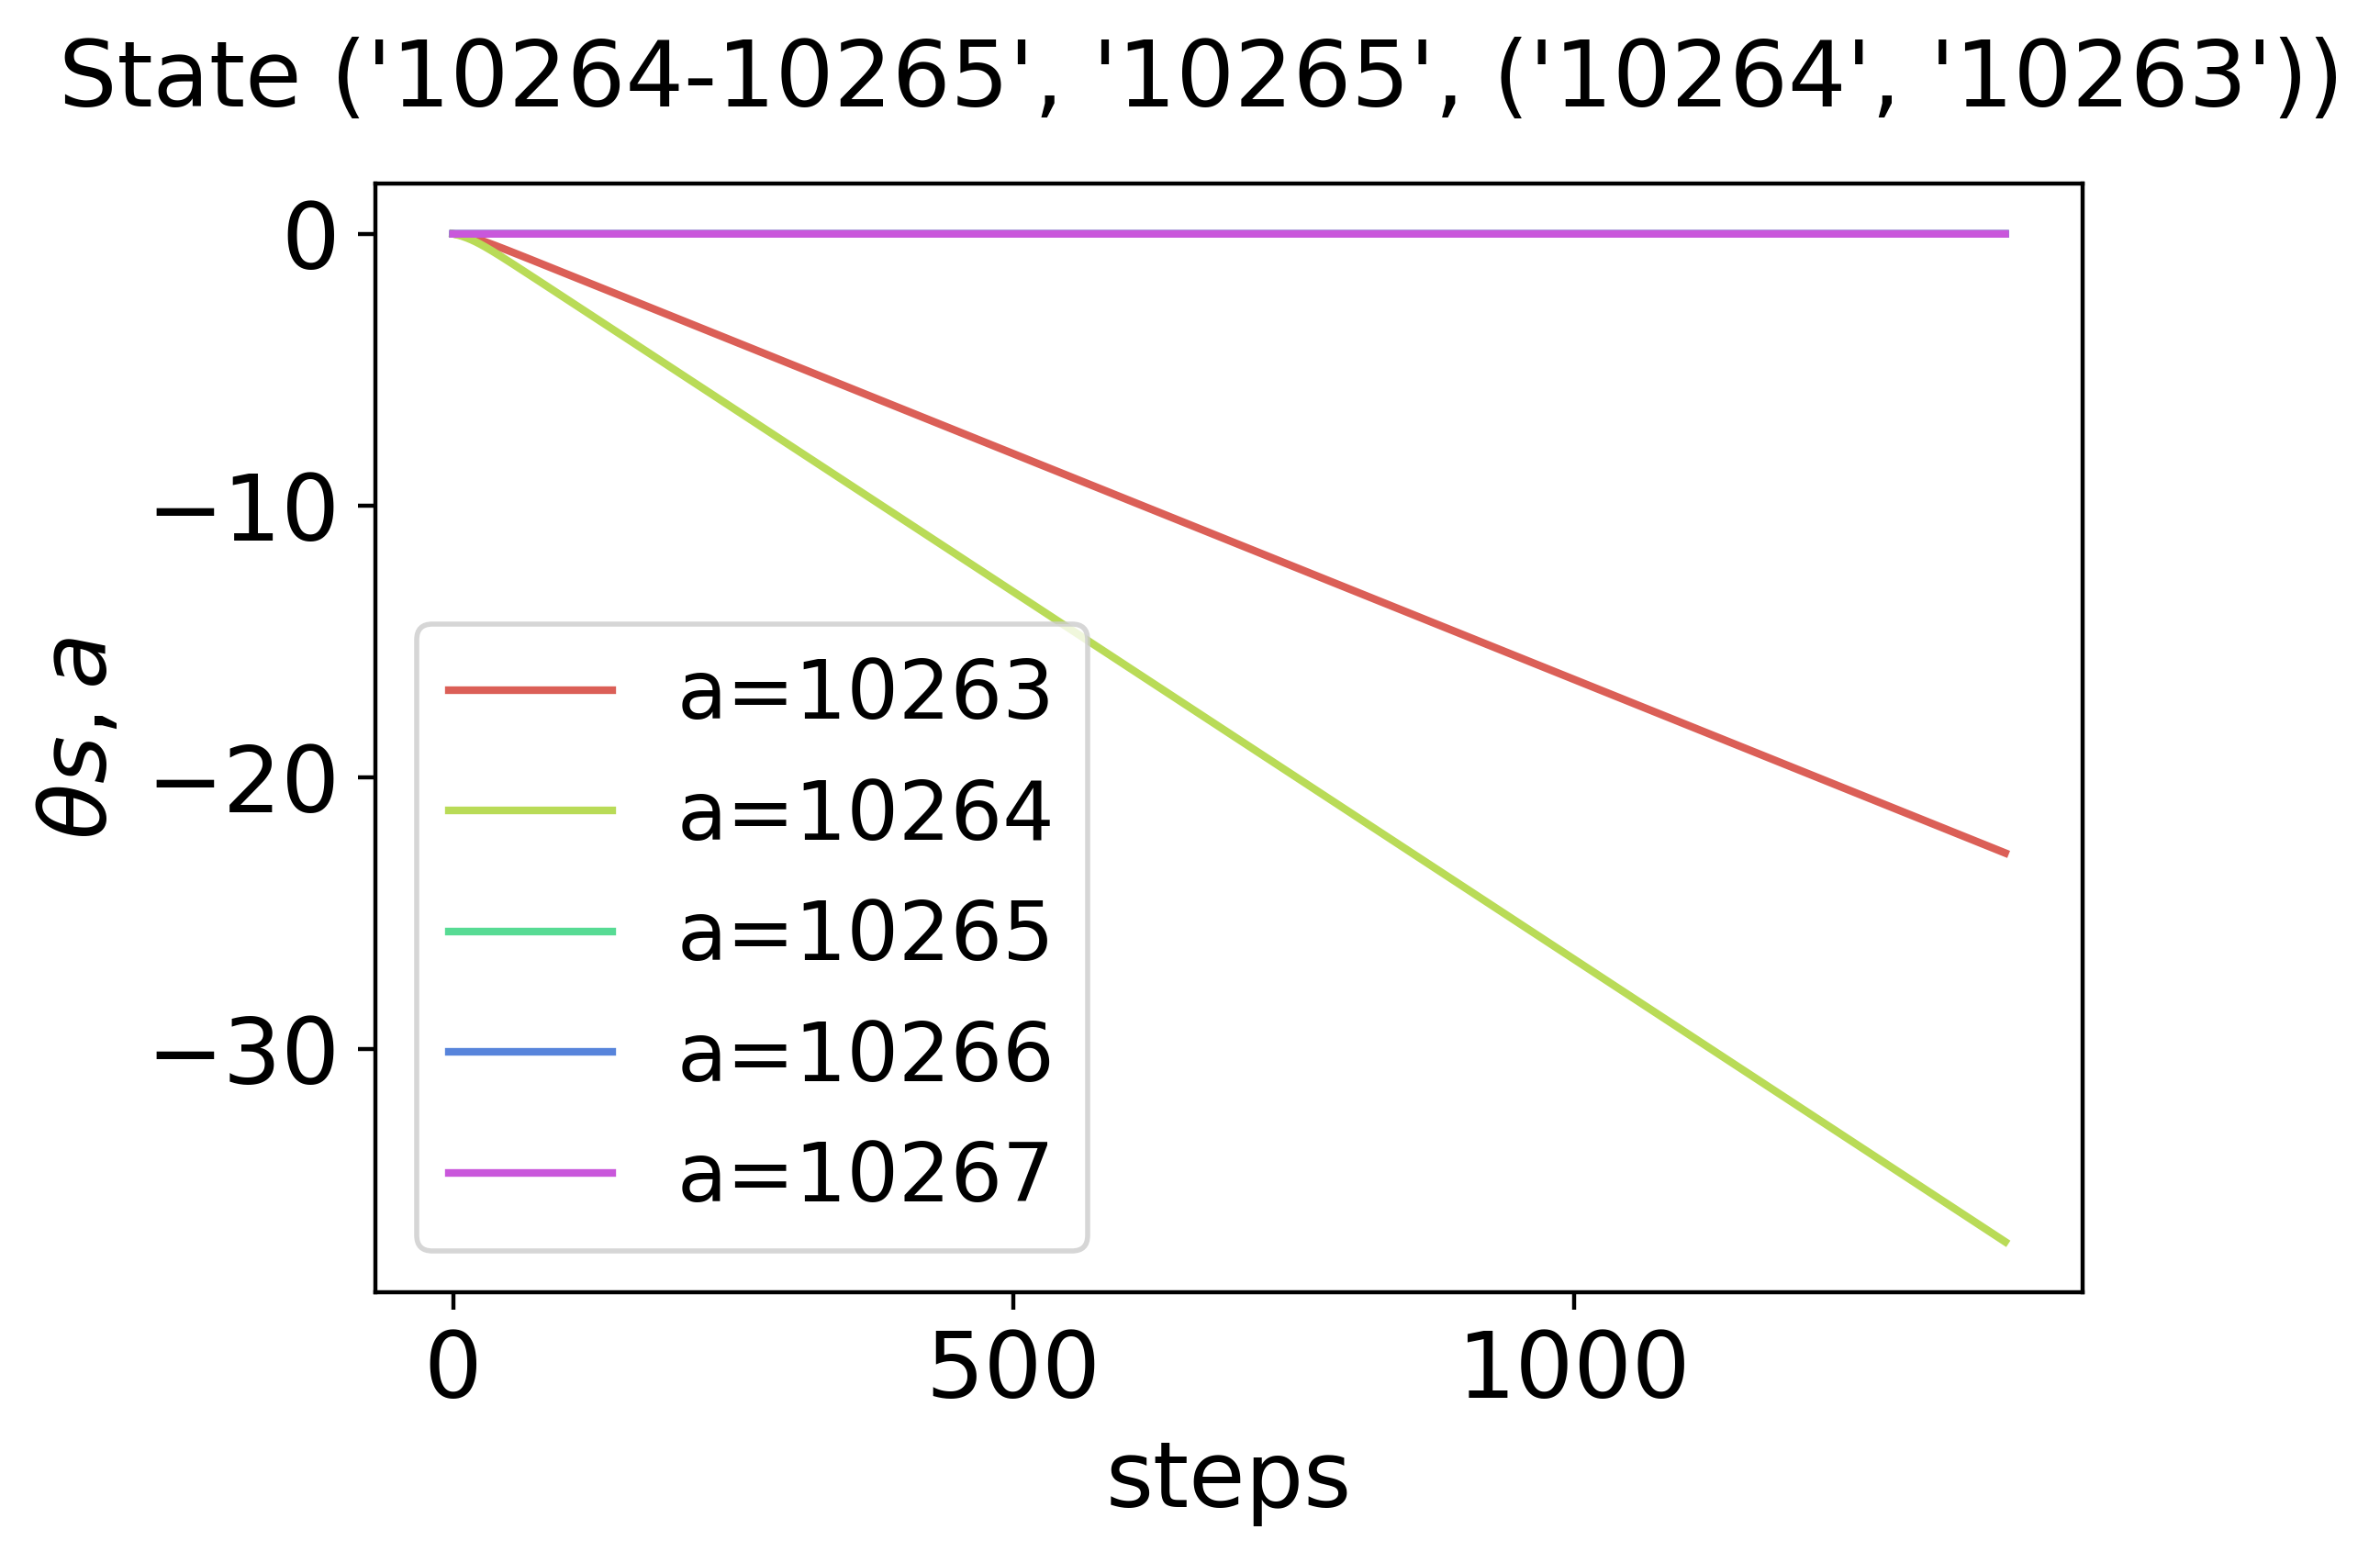
\includegraphics[height=0.27\textwidth,valign=b]{chapters/figures/theta_NPG_state_1.png} \\
        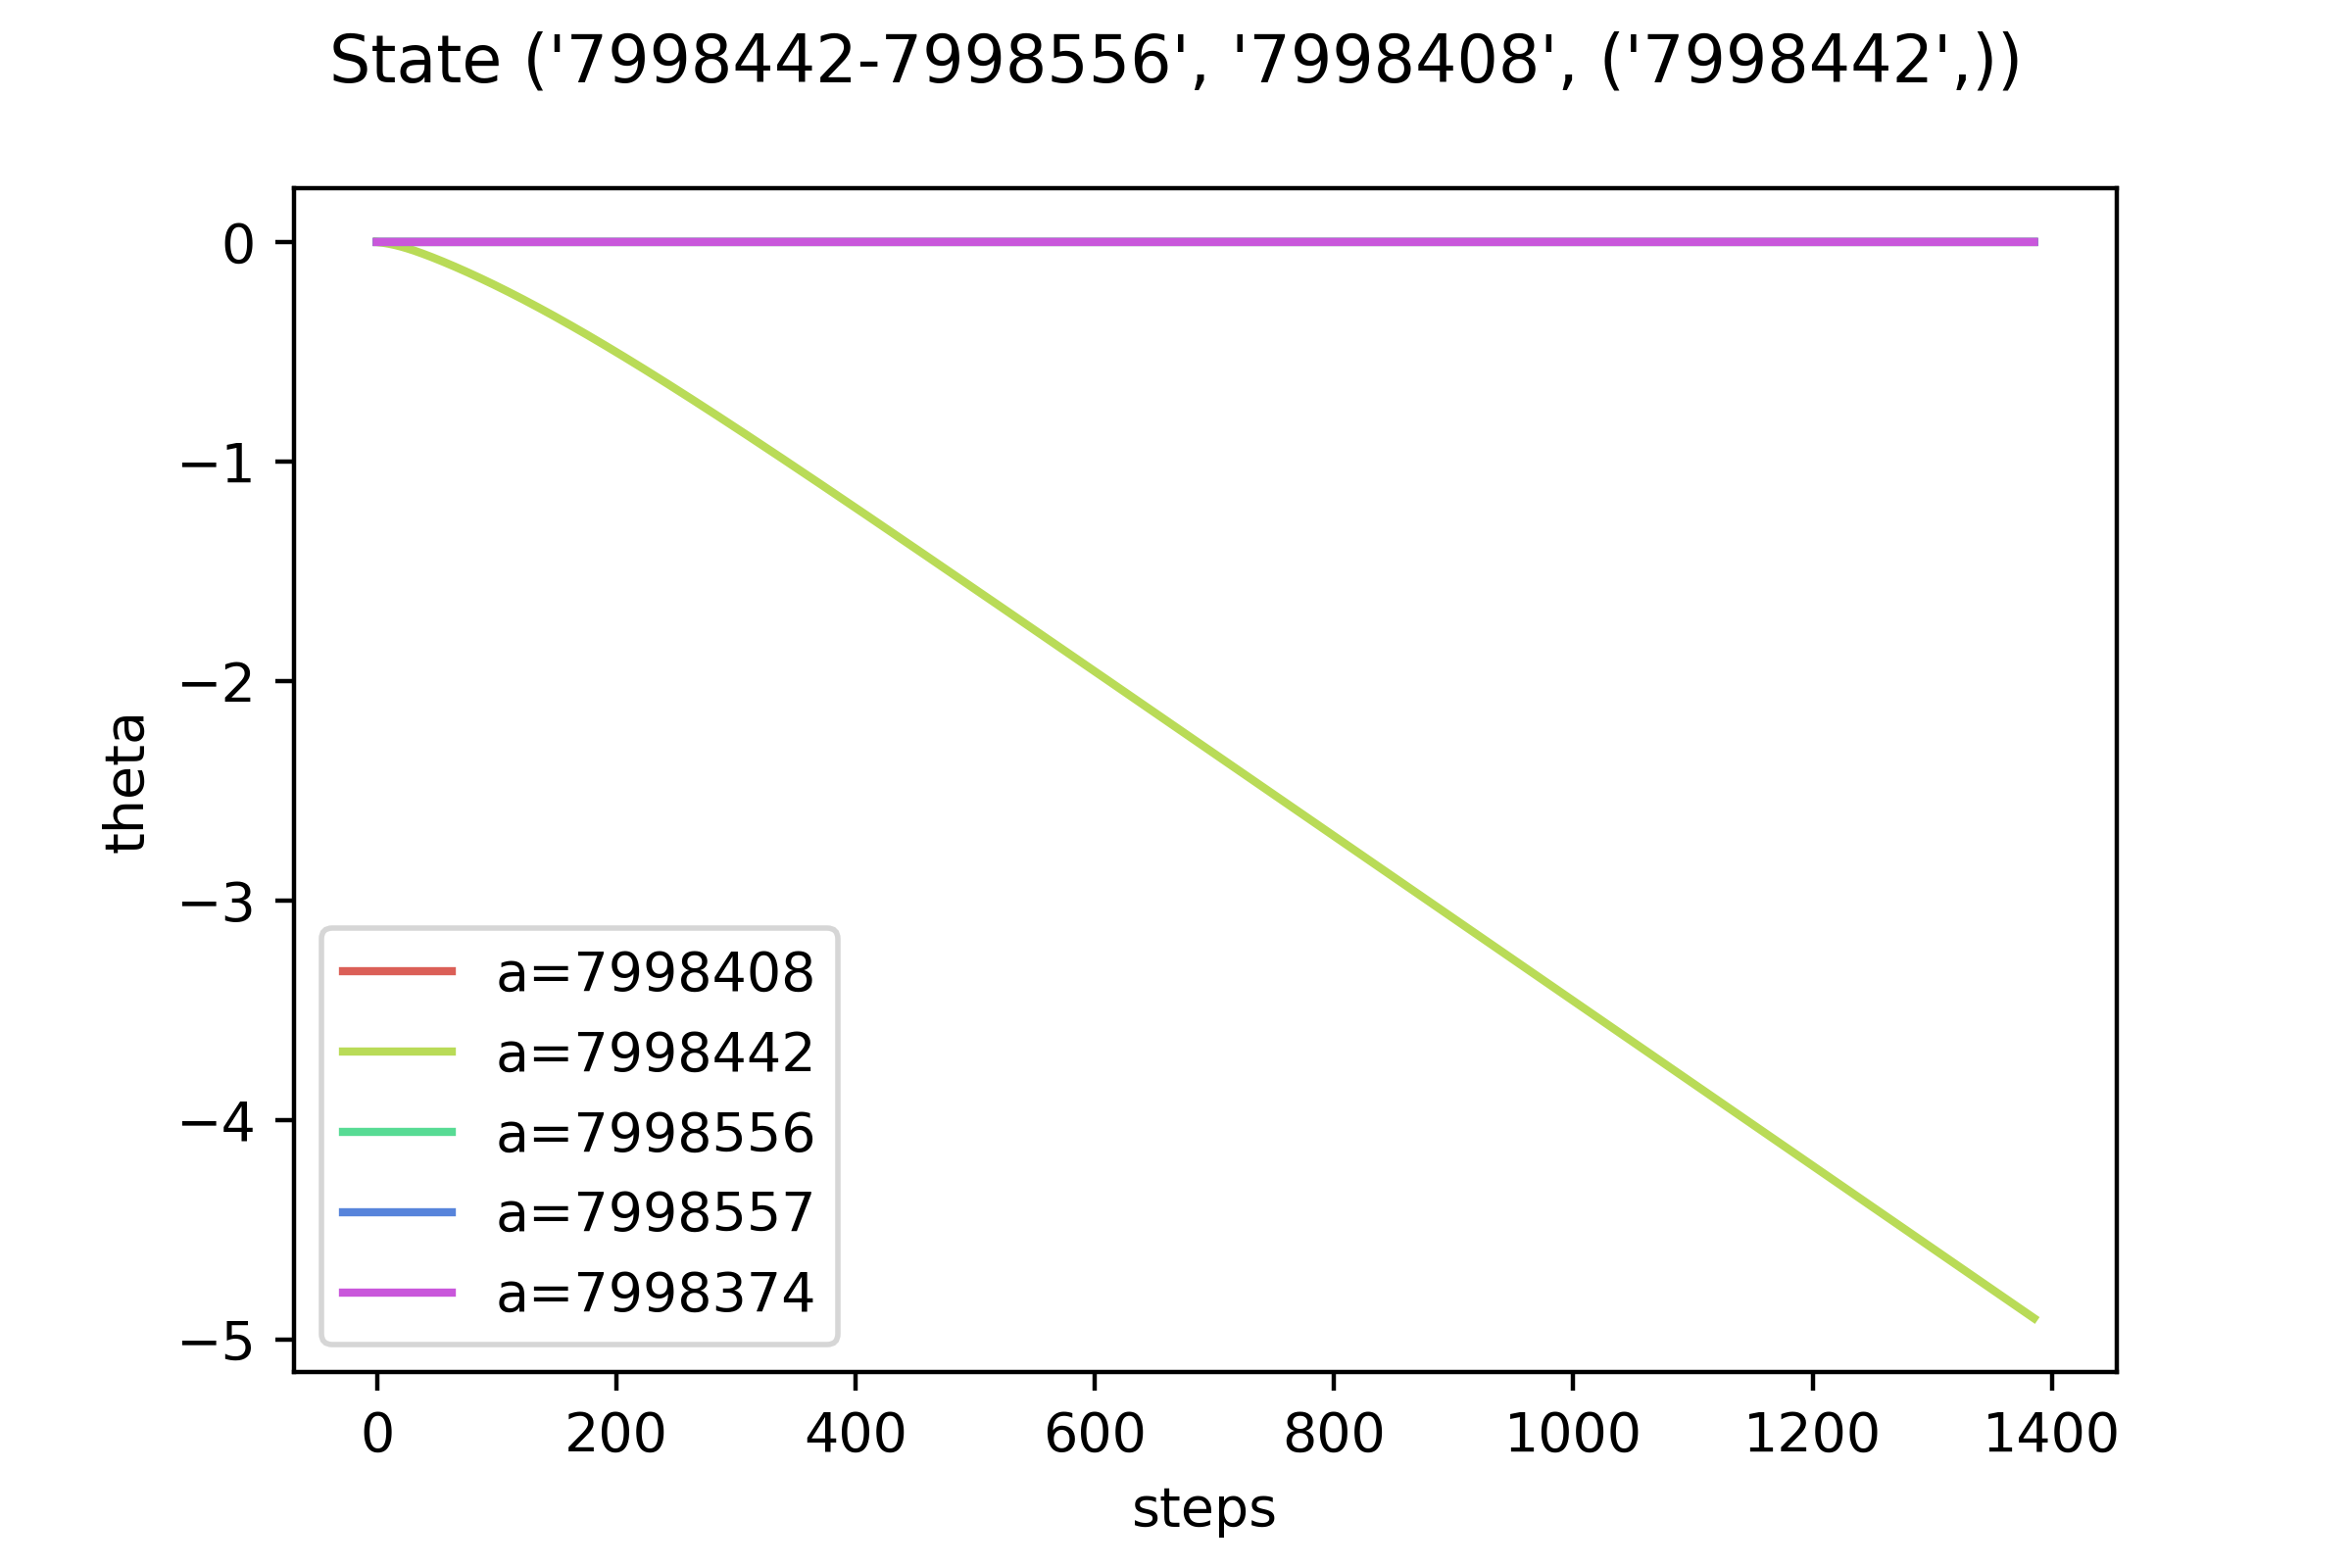
\includegraphics[height=0.27\textwidth,valign=b]{chapters/figures/theta_NPG_state_2.png} &
        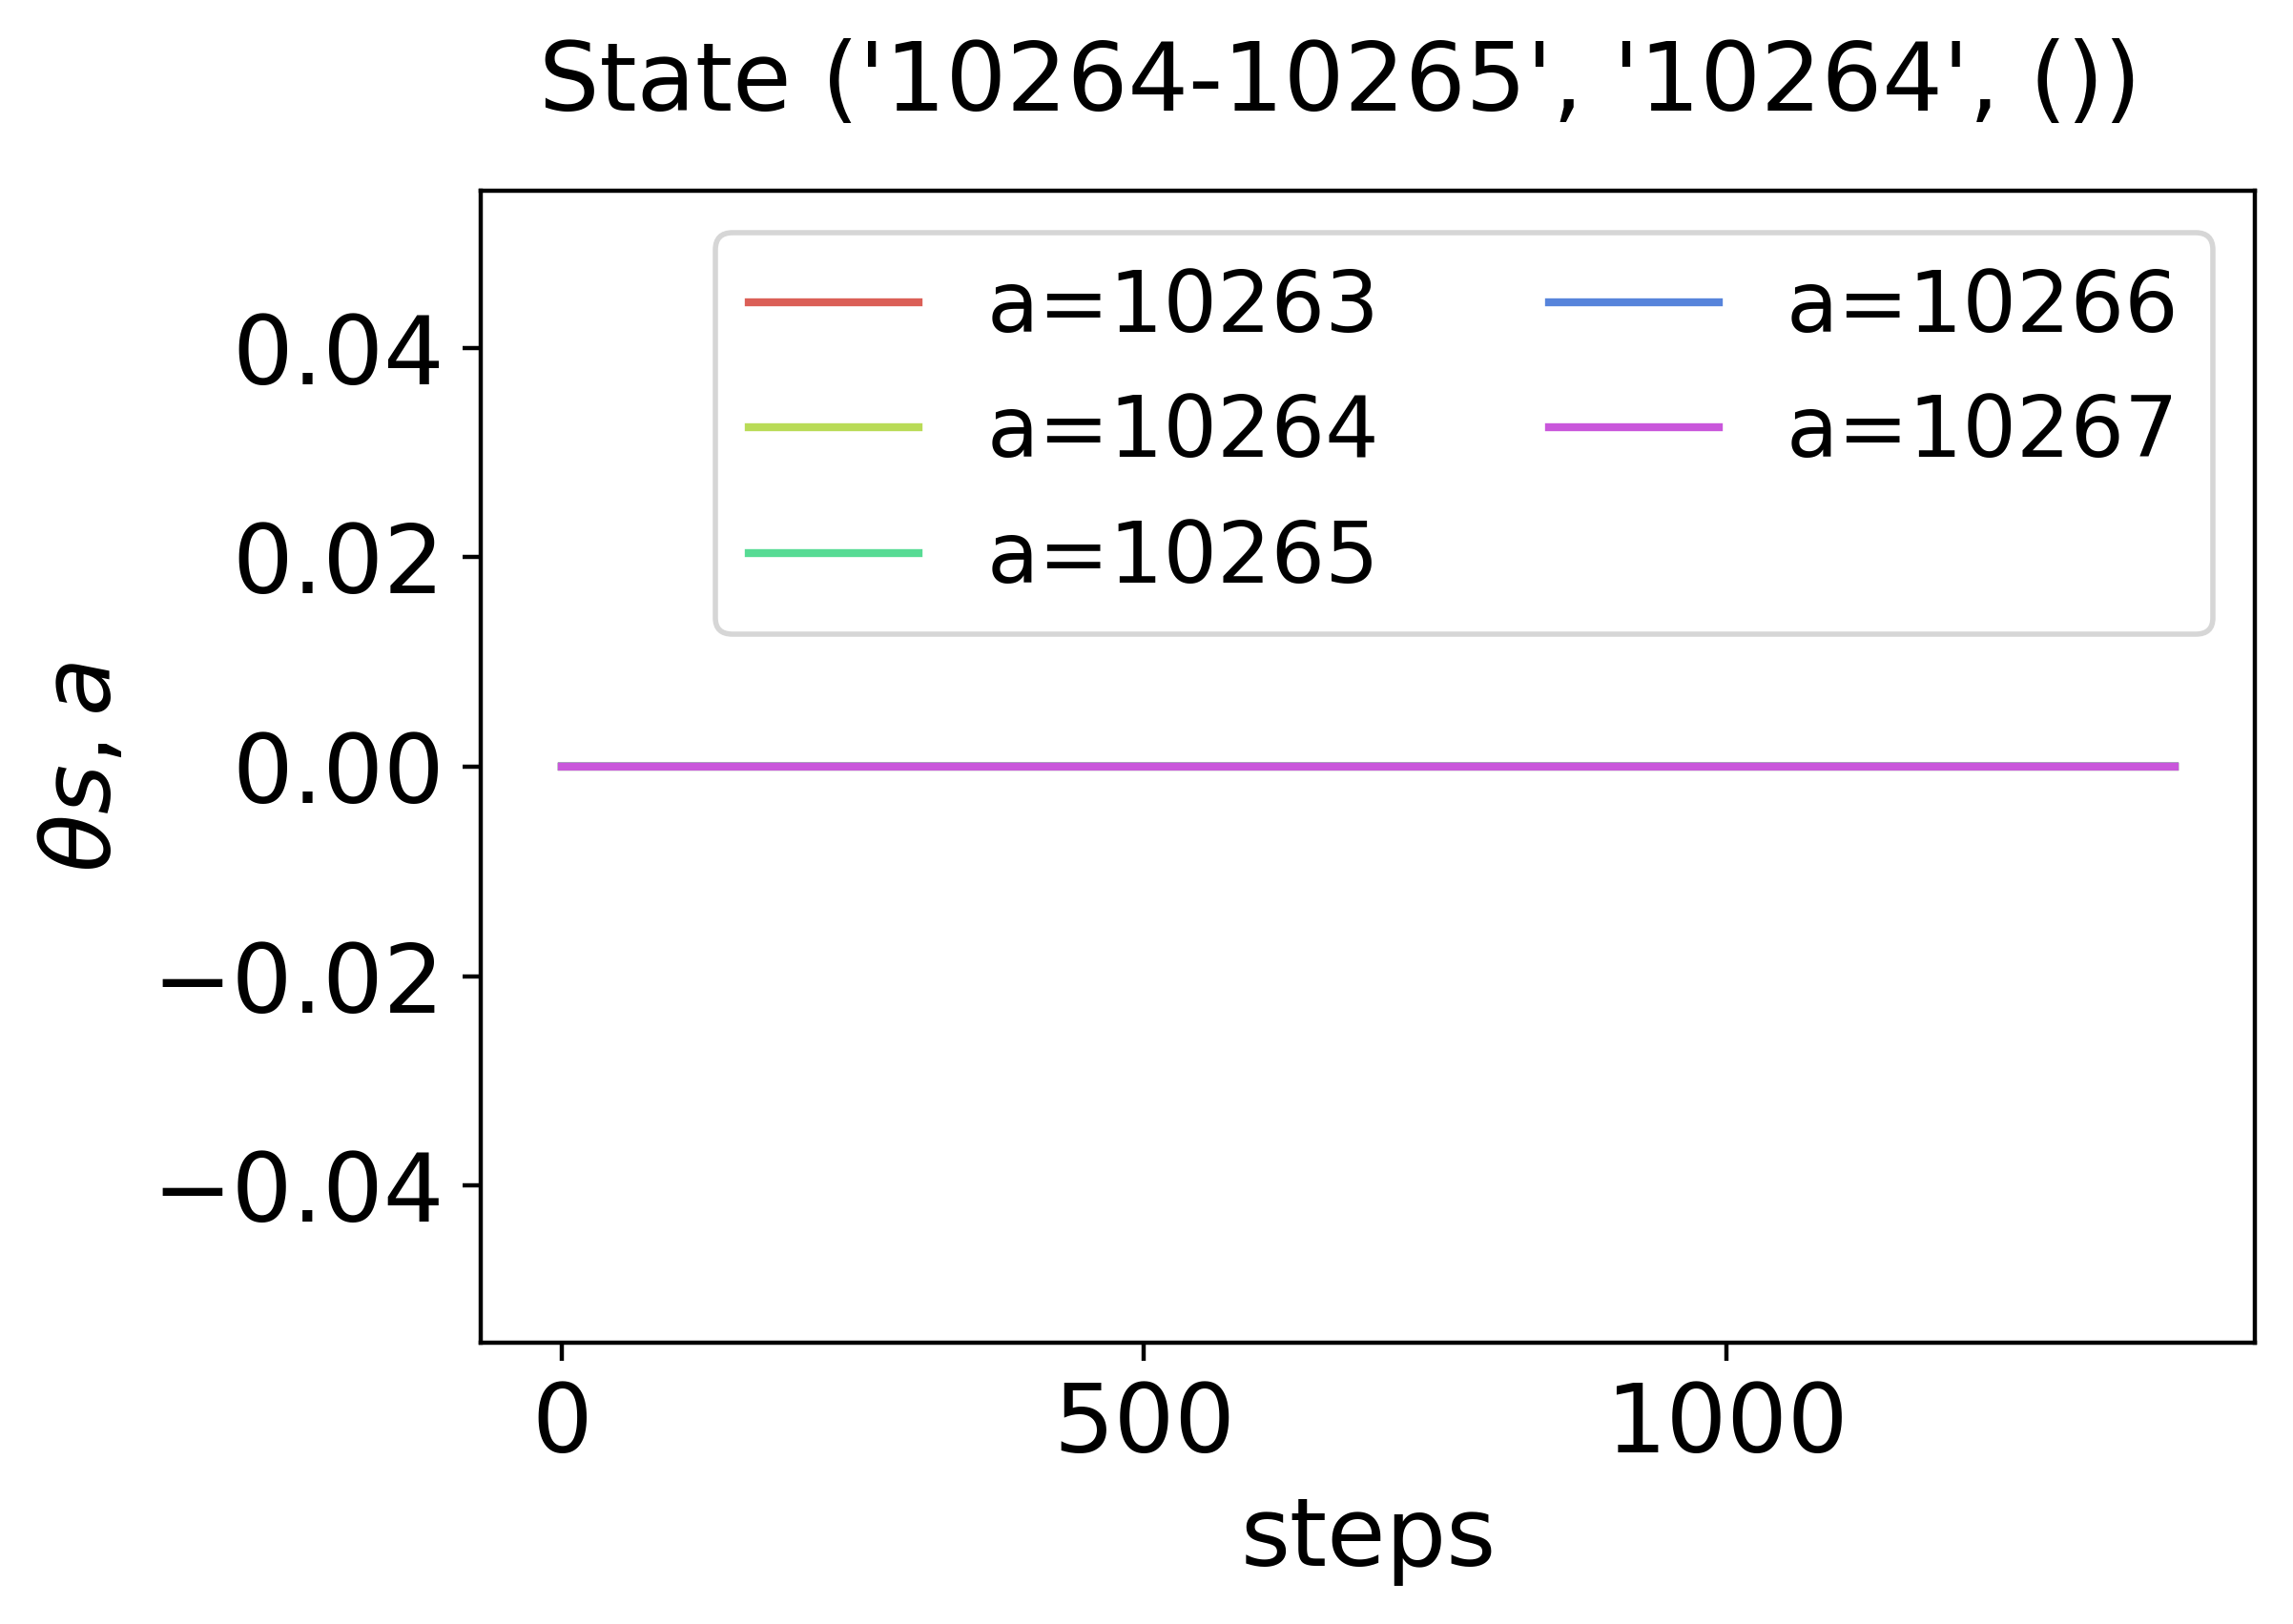
\includegraphics[height=0.27\textwidth,valign=b]{chapters/figures/theta_NPG_state_3.png}
    \end{tabular}
    \caption{Trajectories of the parameters $\boldsymbol \theta$ in the parameters space for \acrshort{npg}, for a specific episode with $5$ initially disconnected substation.}
    \label{fig:sequence-theta-npg}
\end{figure}

\begin{figure}[!htp]
    \centering
    \begin{tabular}{cc}
        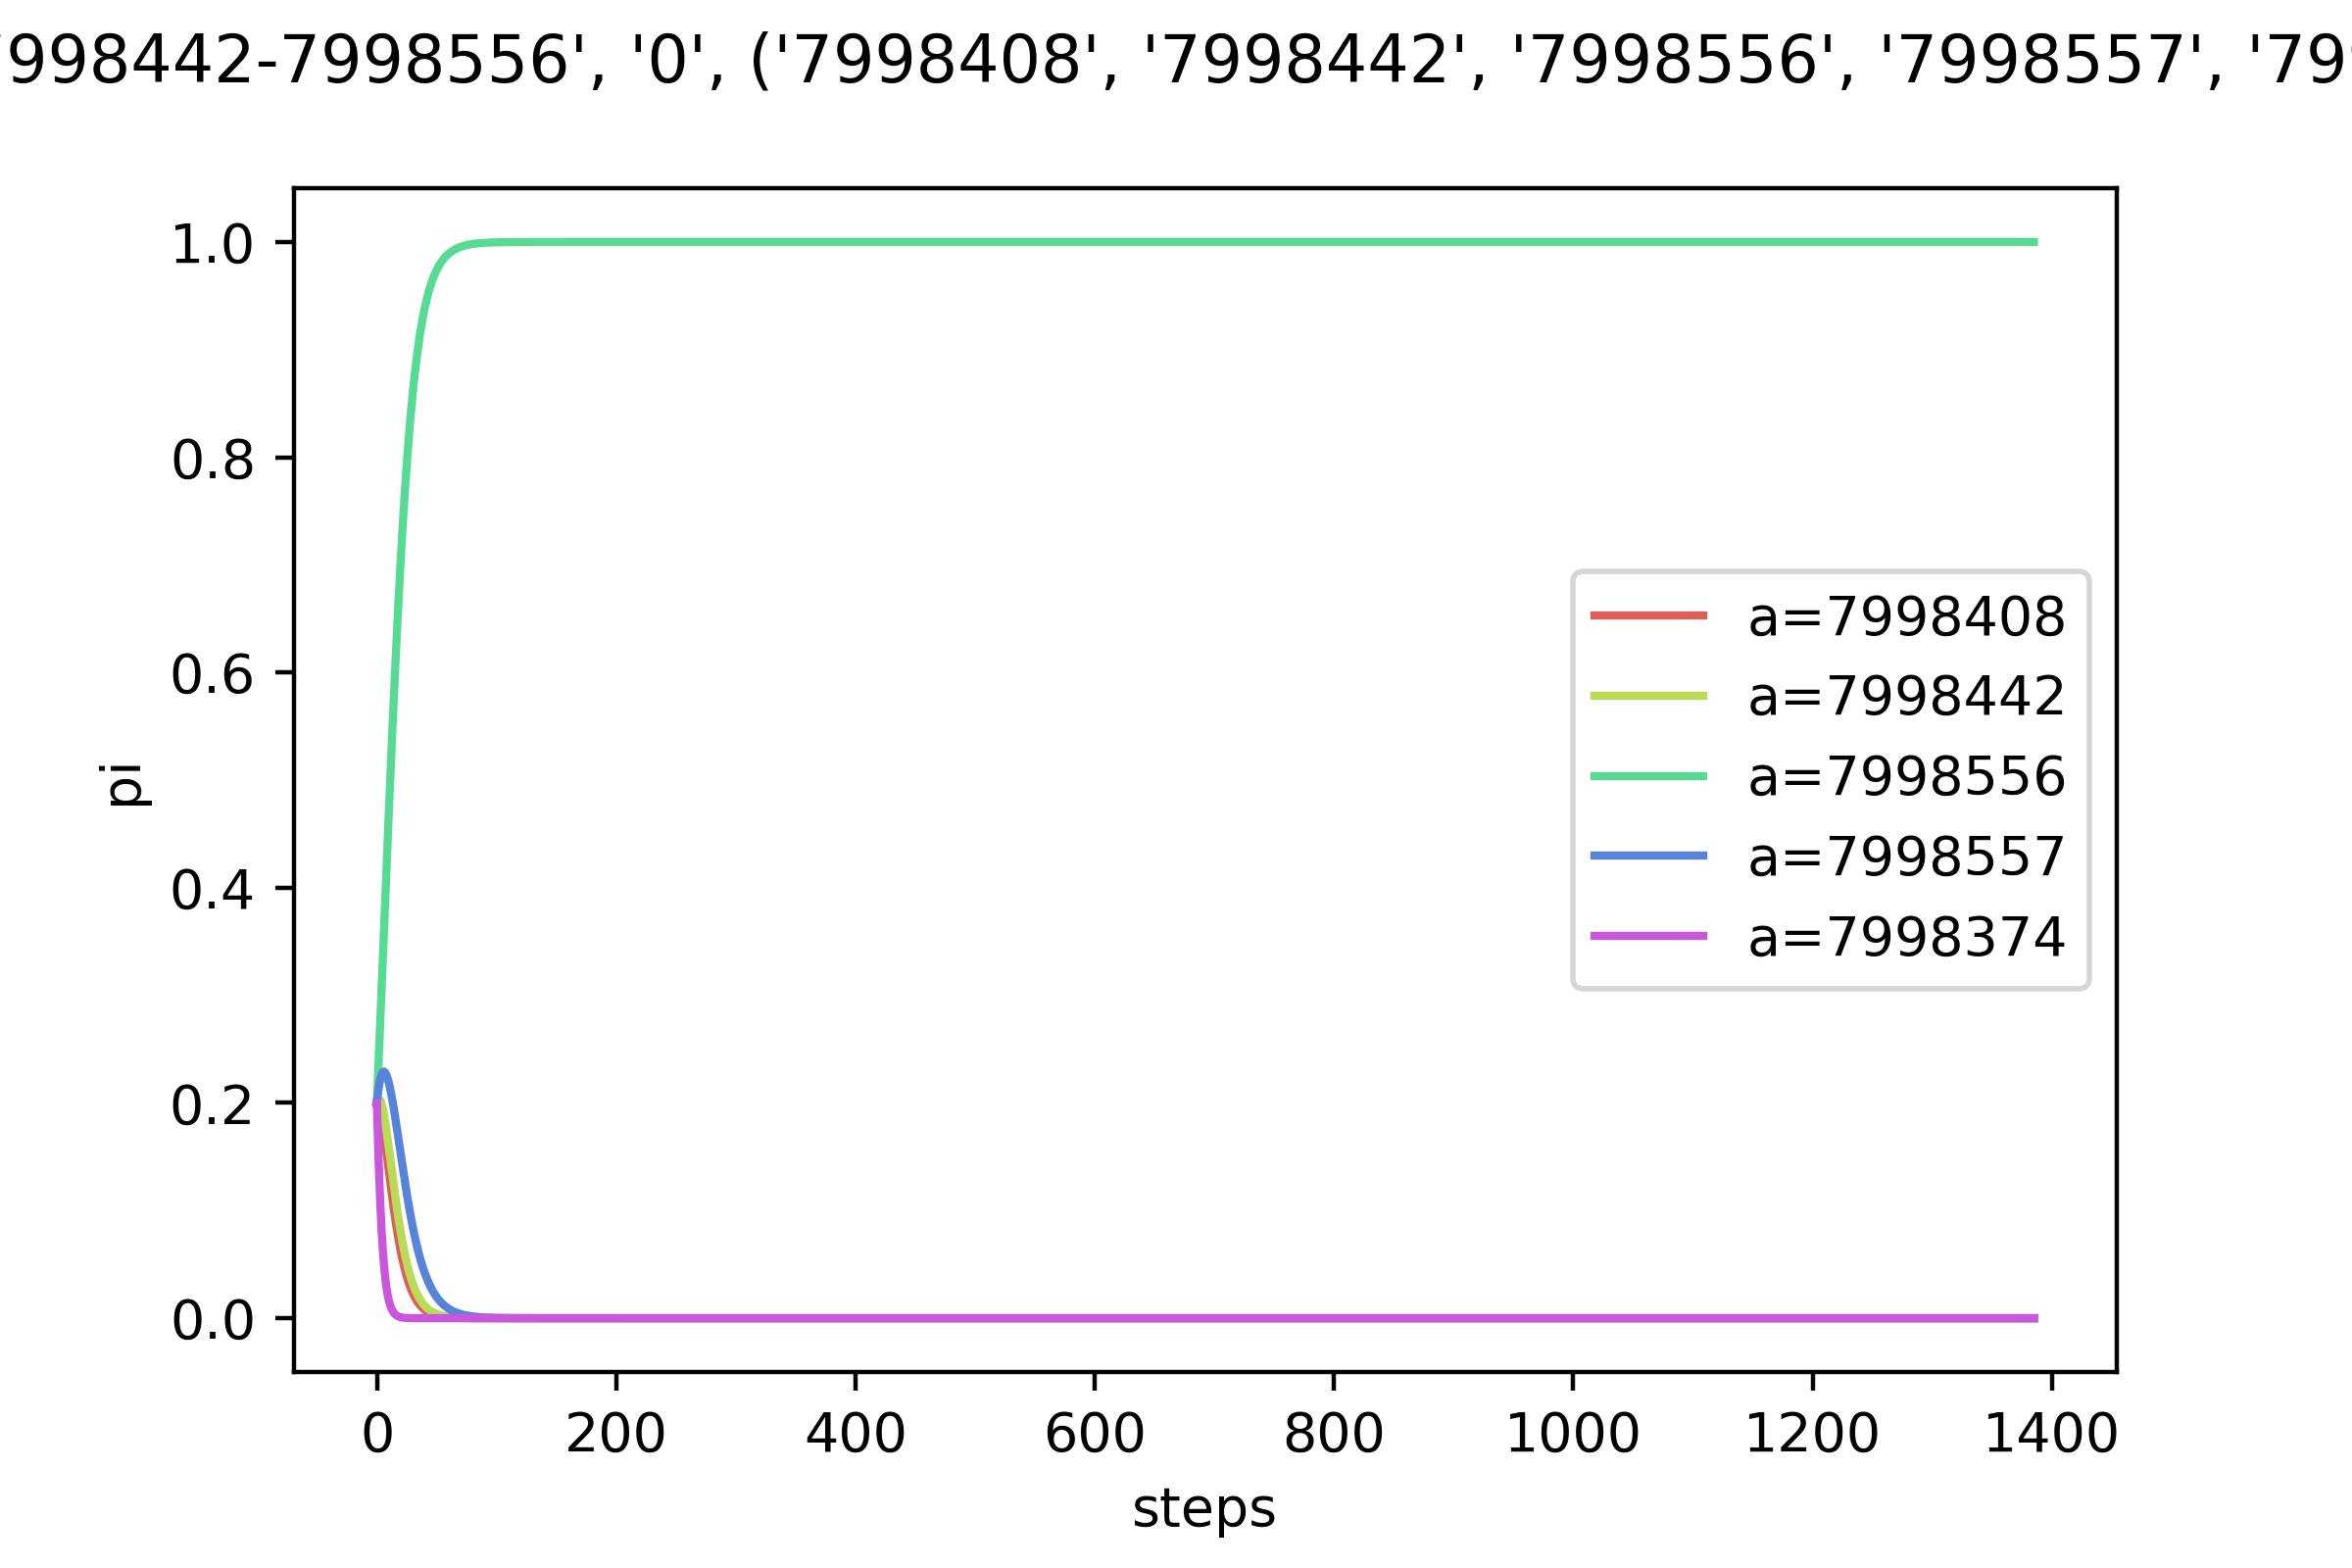
\includegraphics[height=0.27\textwidth,valign=b]{chapters/figures/policy_NPG_state_0.png} &
        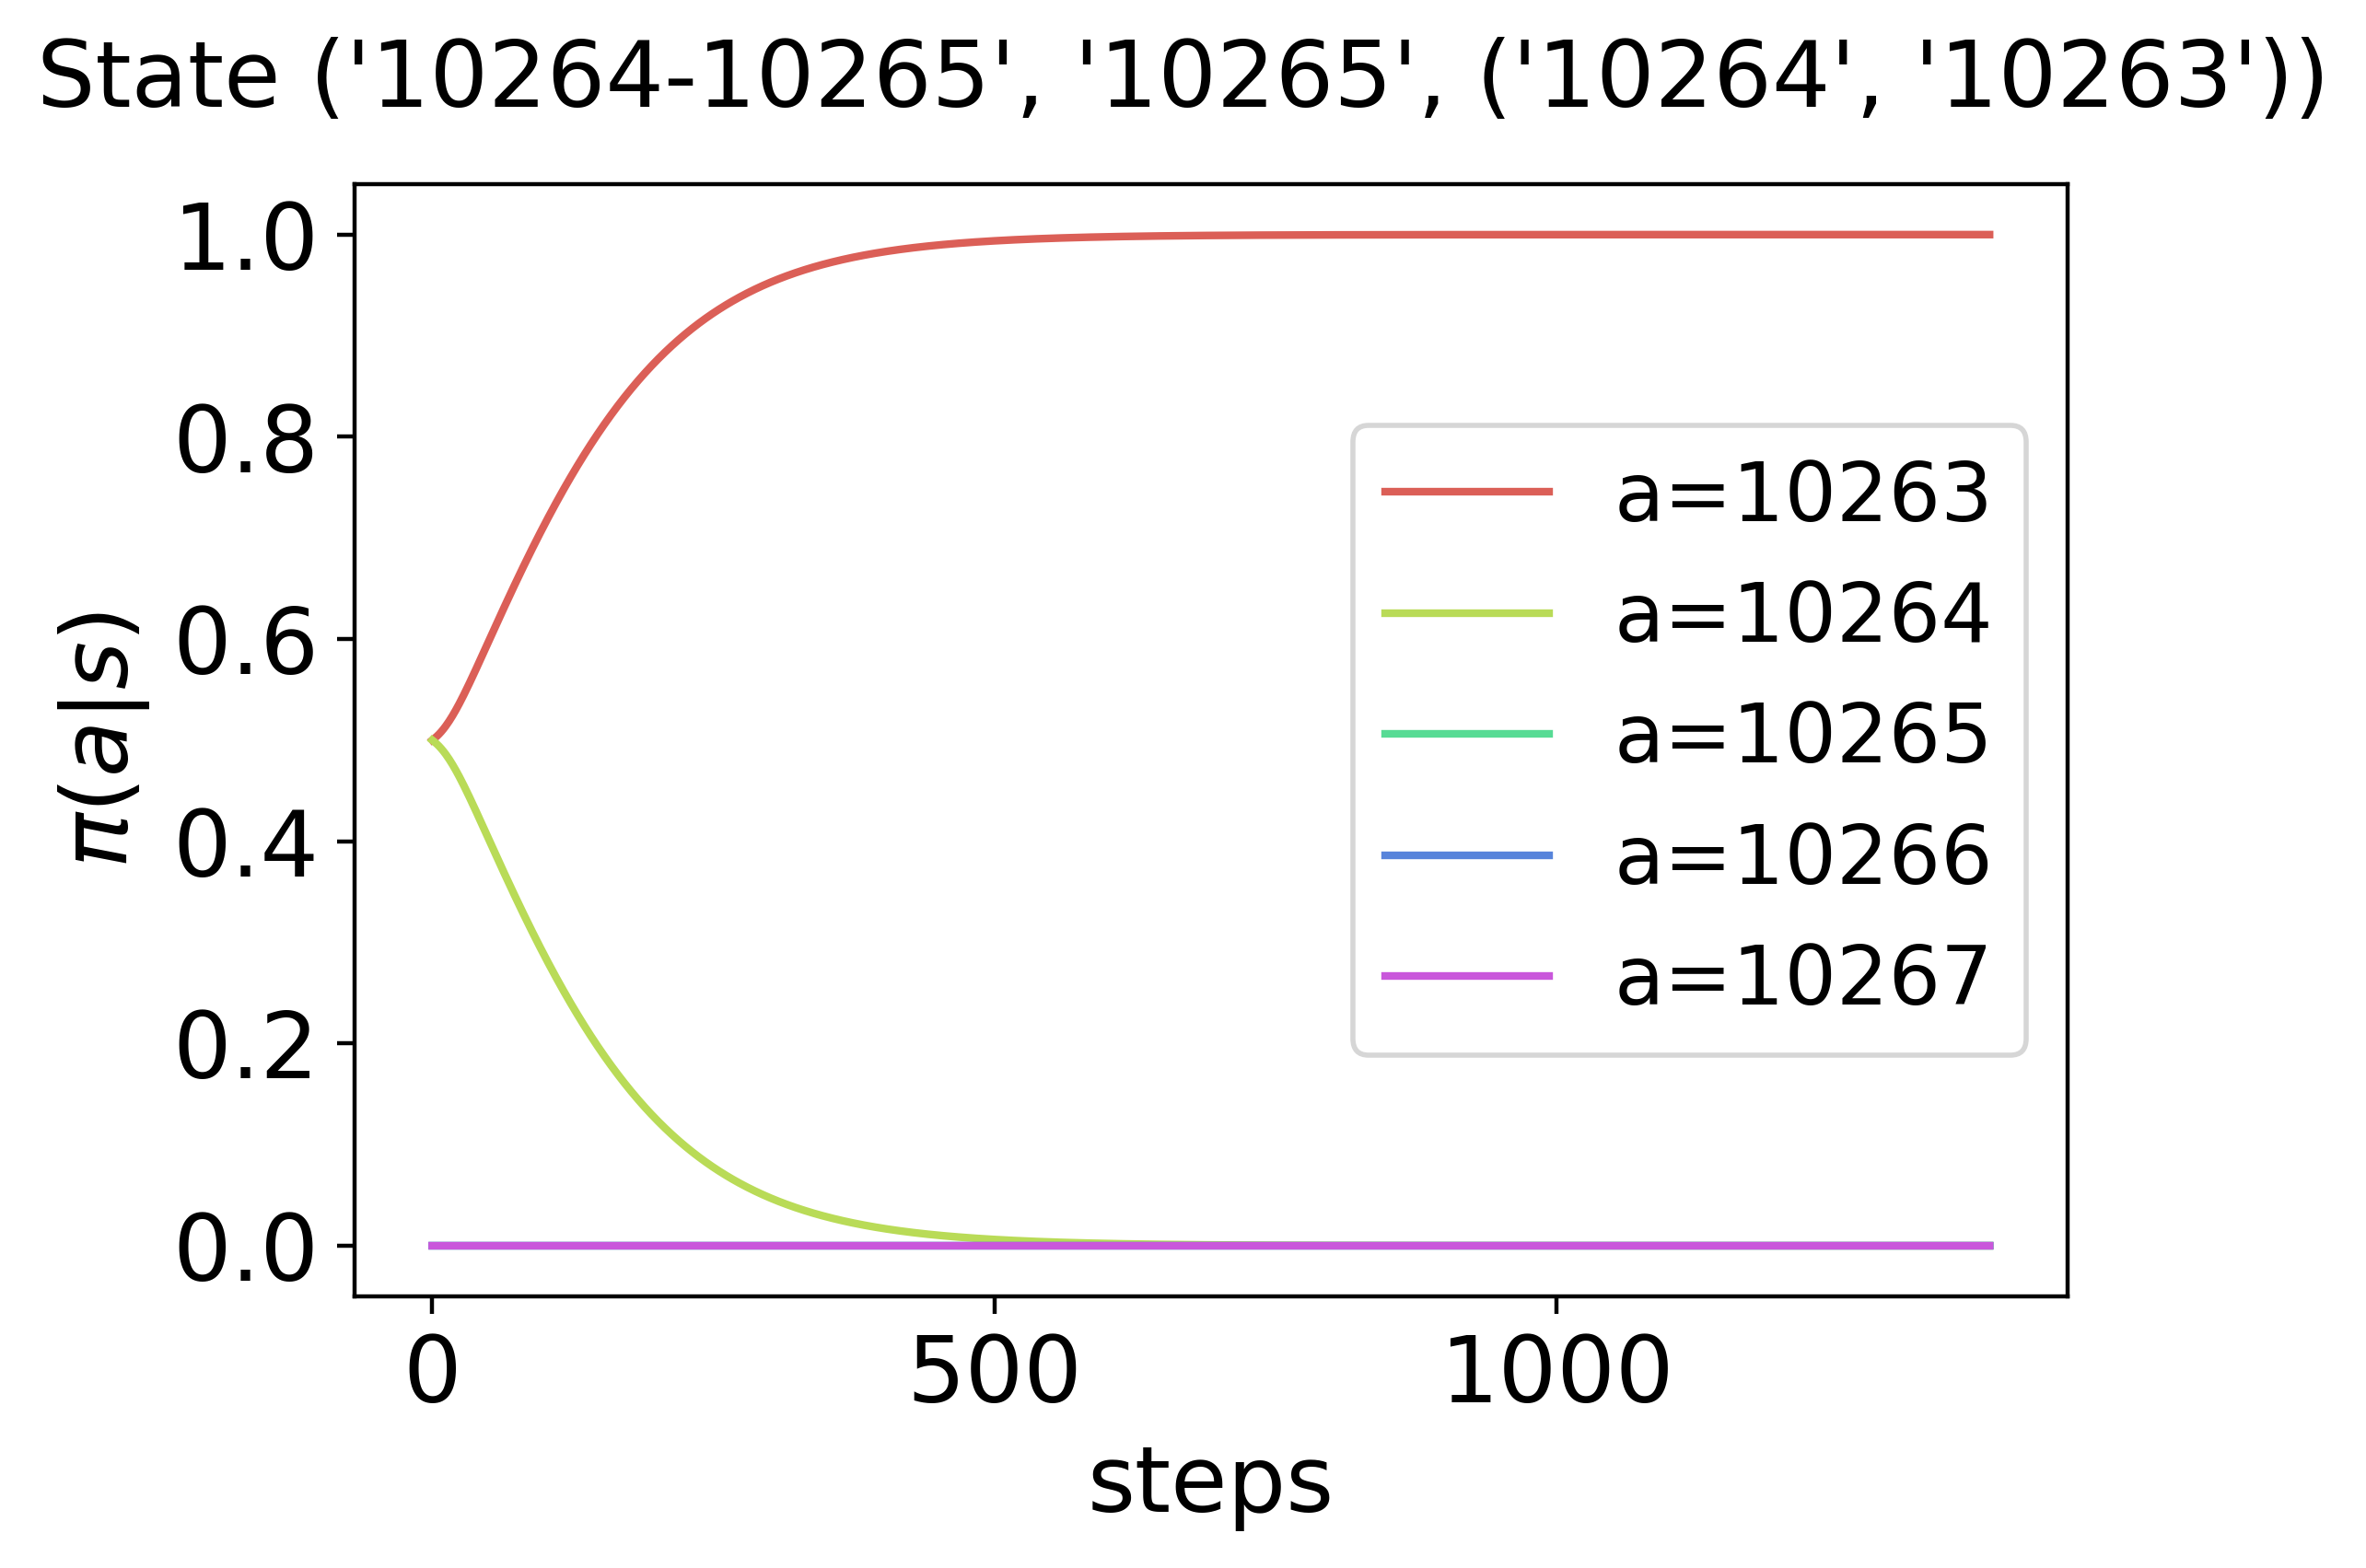
\includegraphics[height=0.27\textwidth,valign=b]{chapters/figures/policy_NPG_state_1.png} \\
        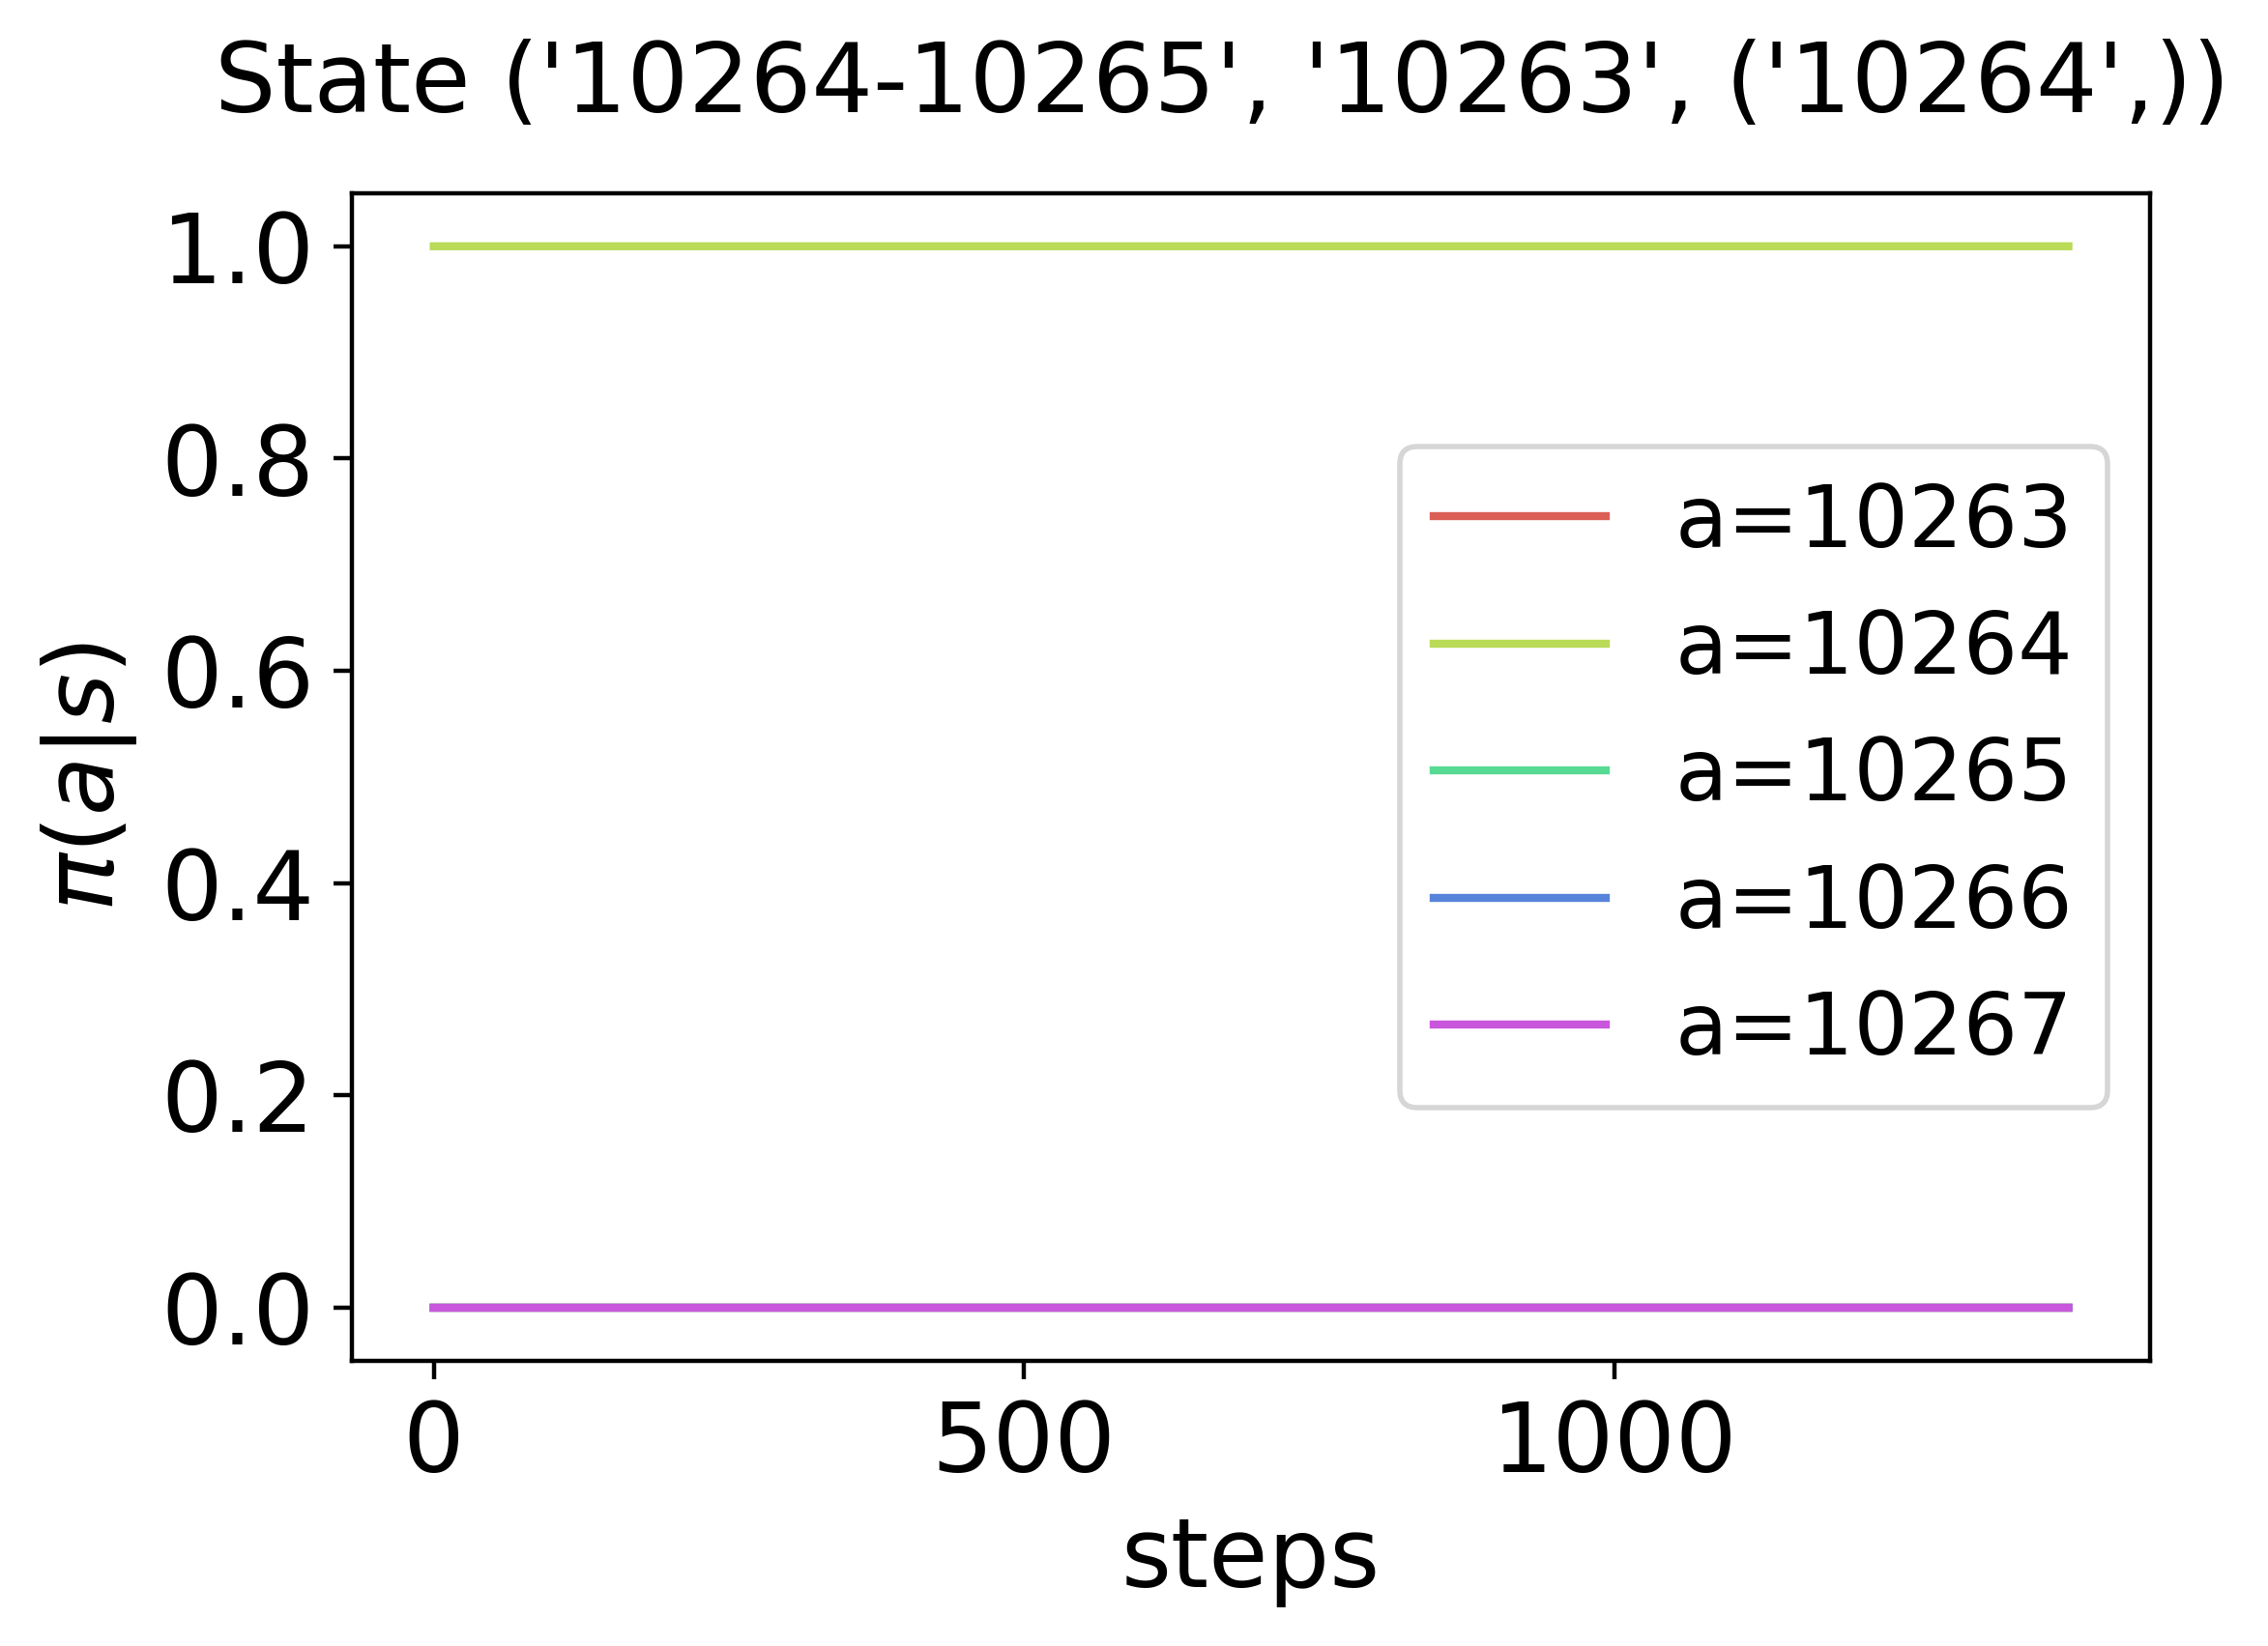
\includegraphics[height=0.27\textwidth,valign=b]{chapters/figures/policy_NPG_state_2.png} &
        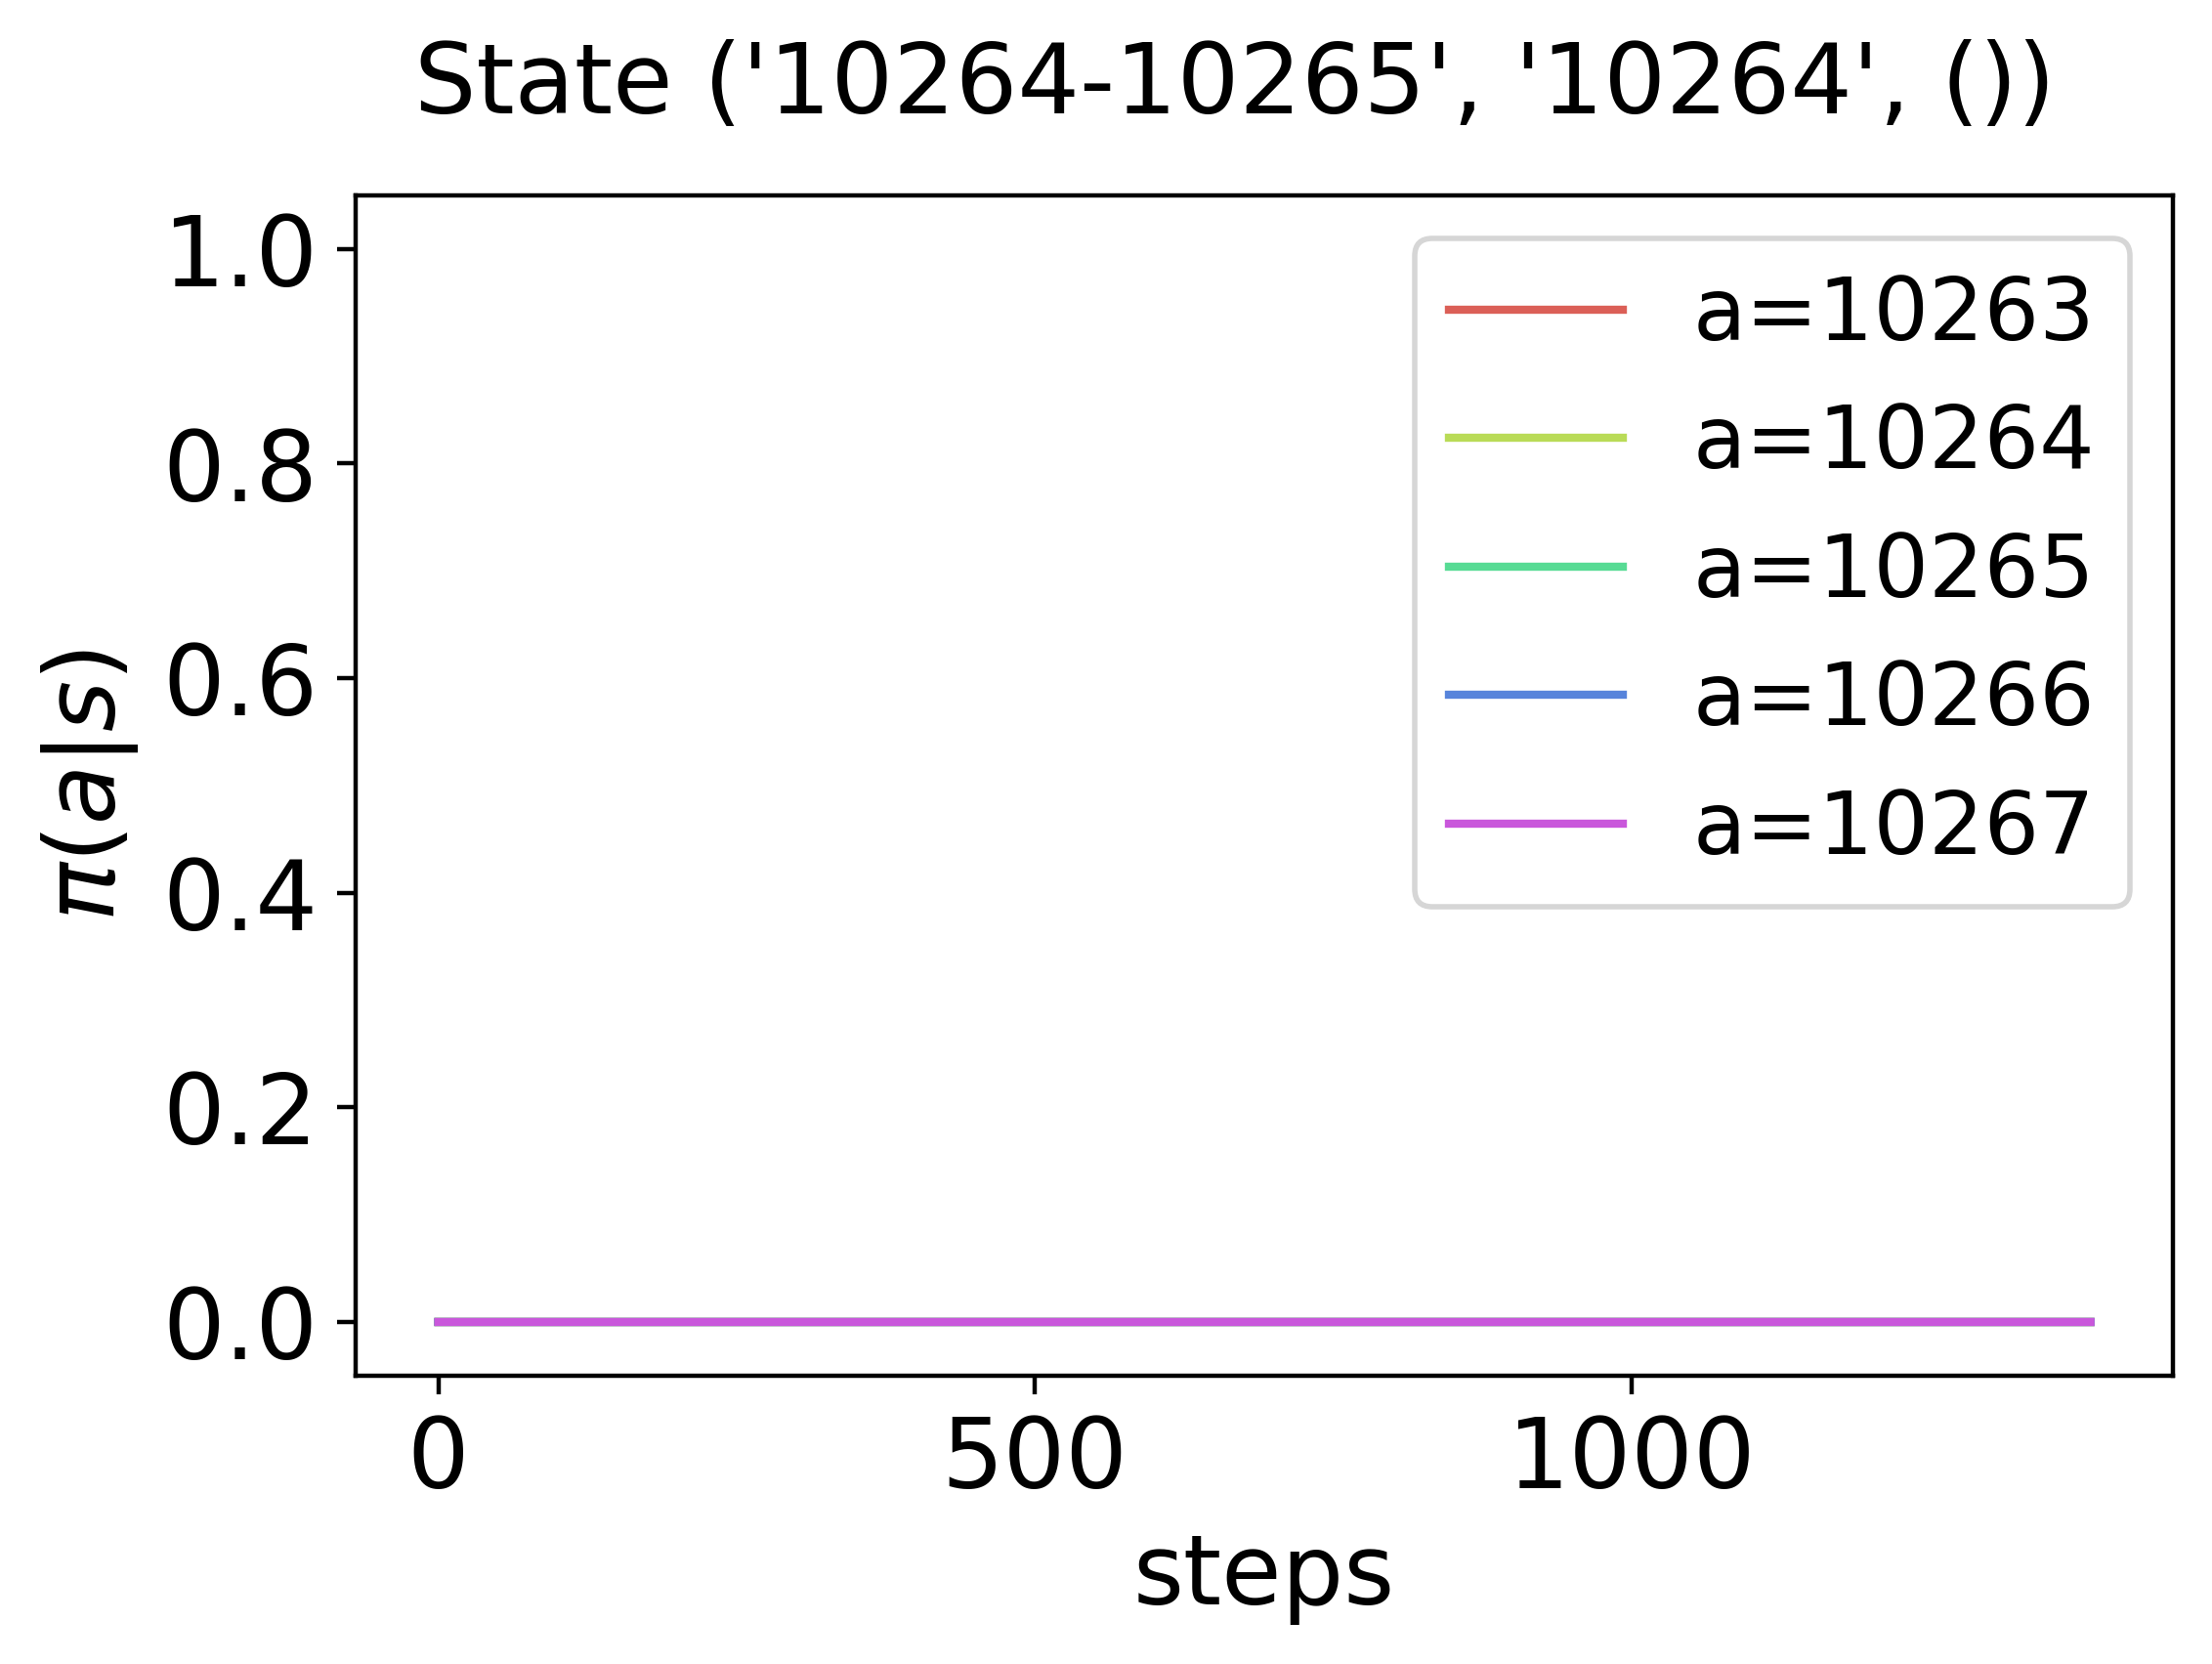
\includegraphics[height=0.27\textwidth,valign=b]{chapters/figures/policy_NPG_state_3.png}
    \end{tabular}
    \caption{Trajectories of the policies $\pi_{\boldsymbol \theta}$ in the policy space for \acrshort{npg}, for a specific episode with $5$ initially disconnected substation.}
    \label{fig:sequence-policies-npg}
\end{figure}

The most important thing to notice in these figures is that all the trajectories are continuous, without sudden turns backward. Going into more detail, in the \acrshort{pg} trajectories of $\boldsymbol \theta$ we can see that one of the parameters grows to infinity, while the others either decrease to infinity or are zero (the latter correspond to actions that cannot be taken in that state). In particular, in the last panel all parameters are zero, since in the terminal state we cannot take any action. Moreover, in the second to last panel we have that again all $\theta$s are zero, because we only have one possible action, so the corresponding $\theta$ is zero, in order for the soft-max policy to be equal to $1$, while the others are zero because they correspond to inadmissible actions. Instead, in the \acrshort{npg} we have that all the parameters $\boldsymbol \theta$ decrease, since we are not following the steepest direction in the parameters space, but the steepest direction with respect to the Fisher metric. Even with rather different values of the parameters $\boldsymbol \theta$, the policies are the same (when compared among them, the difference is in the order of $10^{-2}$), and from the figures we can see that they reached convergence.

Instead, the classic check of seeing if the gradient reached a zero is not applicable in this case: in fact, since we find a stochastic policy, we are not in a corner of the space, in which the gradient is exactly zero, but we are on a side, so it can have values different from zero. Indeed, this is what happens if we look at the gradient matrix: for some states it is not equal to zero, even significantly.

Another check we performed to assess the convergence is to initialize the \acrshort{npg} algorithm with the parameters $\boldsymbol \theta$ found by the \acrshort{pg} algorithm, and vice versa. What we got is that the \acrshort{npg} continues the gradient descent for about another $600$ step, reducing a bit the value of $J_\pi(\boldsymbol \theta)$. Actually, the difference is in the order of $10^{-4}$, which is around the $0.001\%$, so it is negligible. Instead, the \acrshort{pg} algorithm exits immediately the gradient descent loop, as soon as the check on the error is performed, and the values of $J_\pi(\boldsymbol \theta)$ are identical (with a difference of $10^{-10}$), as well as the policy (with a difference of $10^{-15}$).

To check if we reached a global minimum or a local one, since we face a non-convex problem, we also performed some random restarts, with the parameters $\boldsymbol \theta$ initialized from a standard normal distribution $\mathcal N(0,1)$. What happens is that each time the algorithm converges to the exact same policy, so we are quite confident that we reached a global minimum. The references \cite{Bhandari2019, bhandari2020note} show that, under some specific conditions, the policy gradient performance measure $J_\pi(\boldsymbol \theta)$ has a unique global minimum, even if it is non-convex. Indeed, it excludes that the performance measure can have another minimum that can be reached from a different initial condition. Given our results, our model could be in this class of problems, but we have not verified, as that was not our purpose.

% Fai i grafi con gli stati con i path di bisezione e di policy gradient (intensità colore in base alla probabilità): così si può vedere che sono diversi.

Since we computed the policy matrix for all the various bisection algorithms, we were able to compute the exact value of $J_\pi (\boldsymbol \theta)$ for all of them, and we were able to make an effective comparison among all the algorithms. In \autoref{fig:comparison-graph}, we can see the values of $J_\pi(\boldsymbol \theta)$ computed by the various algorithms for different numbers of initially disconnected substations. We selected an electrical line of Trieste's power grid, and keeping fixed the initial position of the technician and the last remotely controlled substation, we moved the first remotely controlled substation of one substation each time, in order to incrementally increase by one the number of initially disconnected substations.
% Anche nel comparison graph bisognerebbe dire che J è calcolato solo per i guasti sui cavi
We can clearly see that the policy gradient algorithms are the better ones, with the \acrshort{npg} a little better with higher numbers of disconnected substations. Instead, the different bisection algorithms perform almost the same.

\begin{figure}[htb]
    \centering
    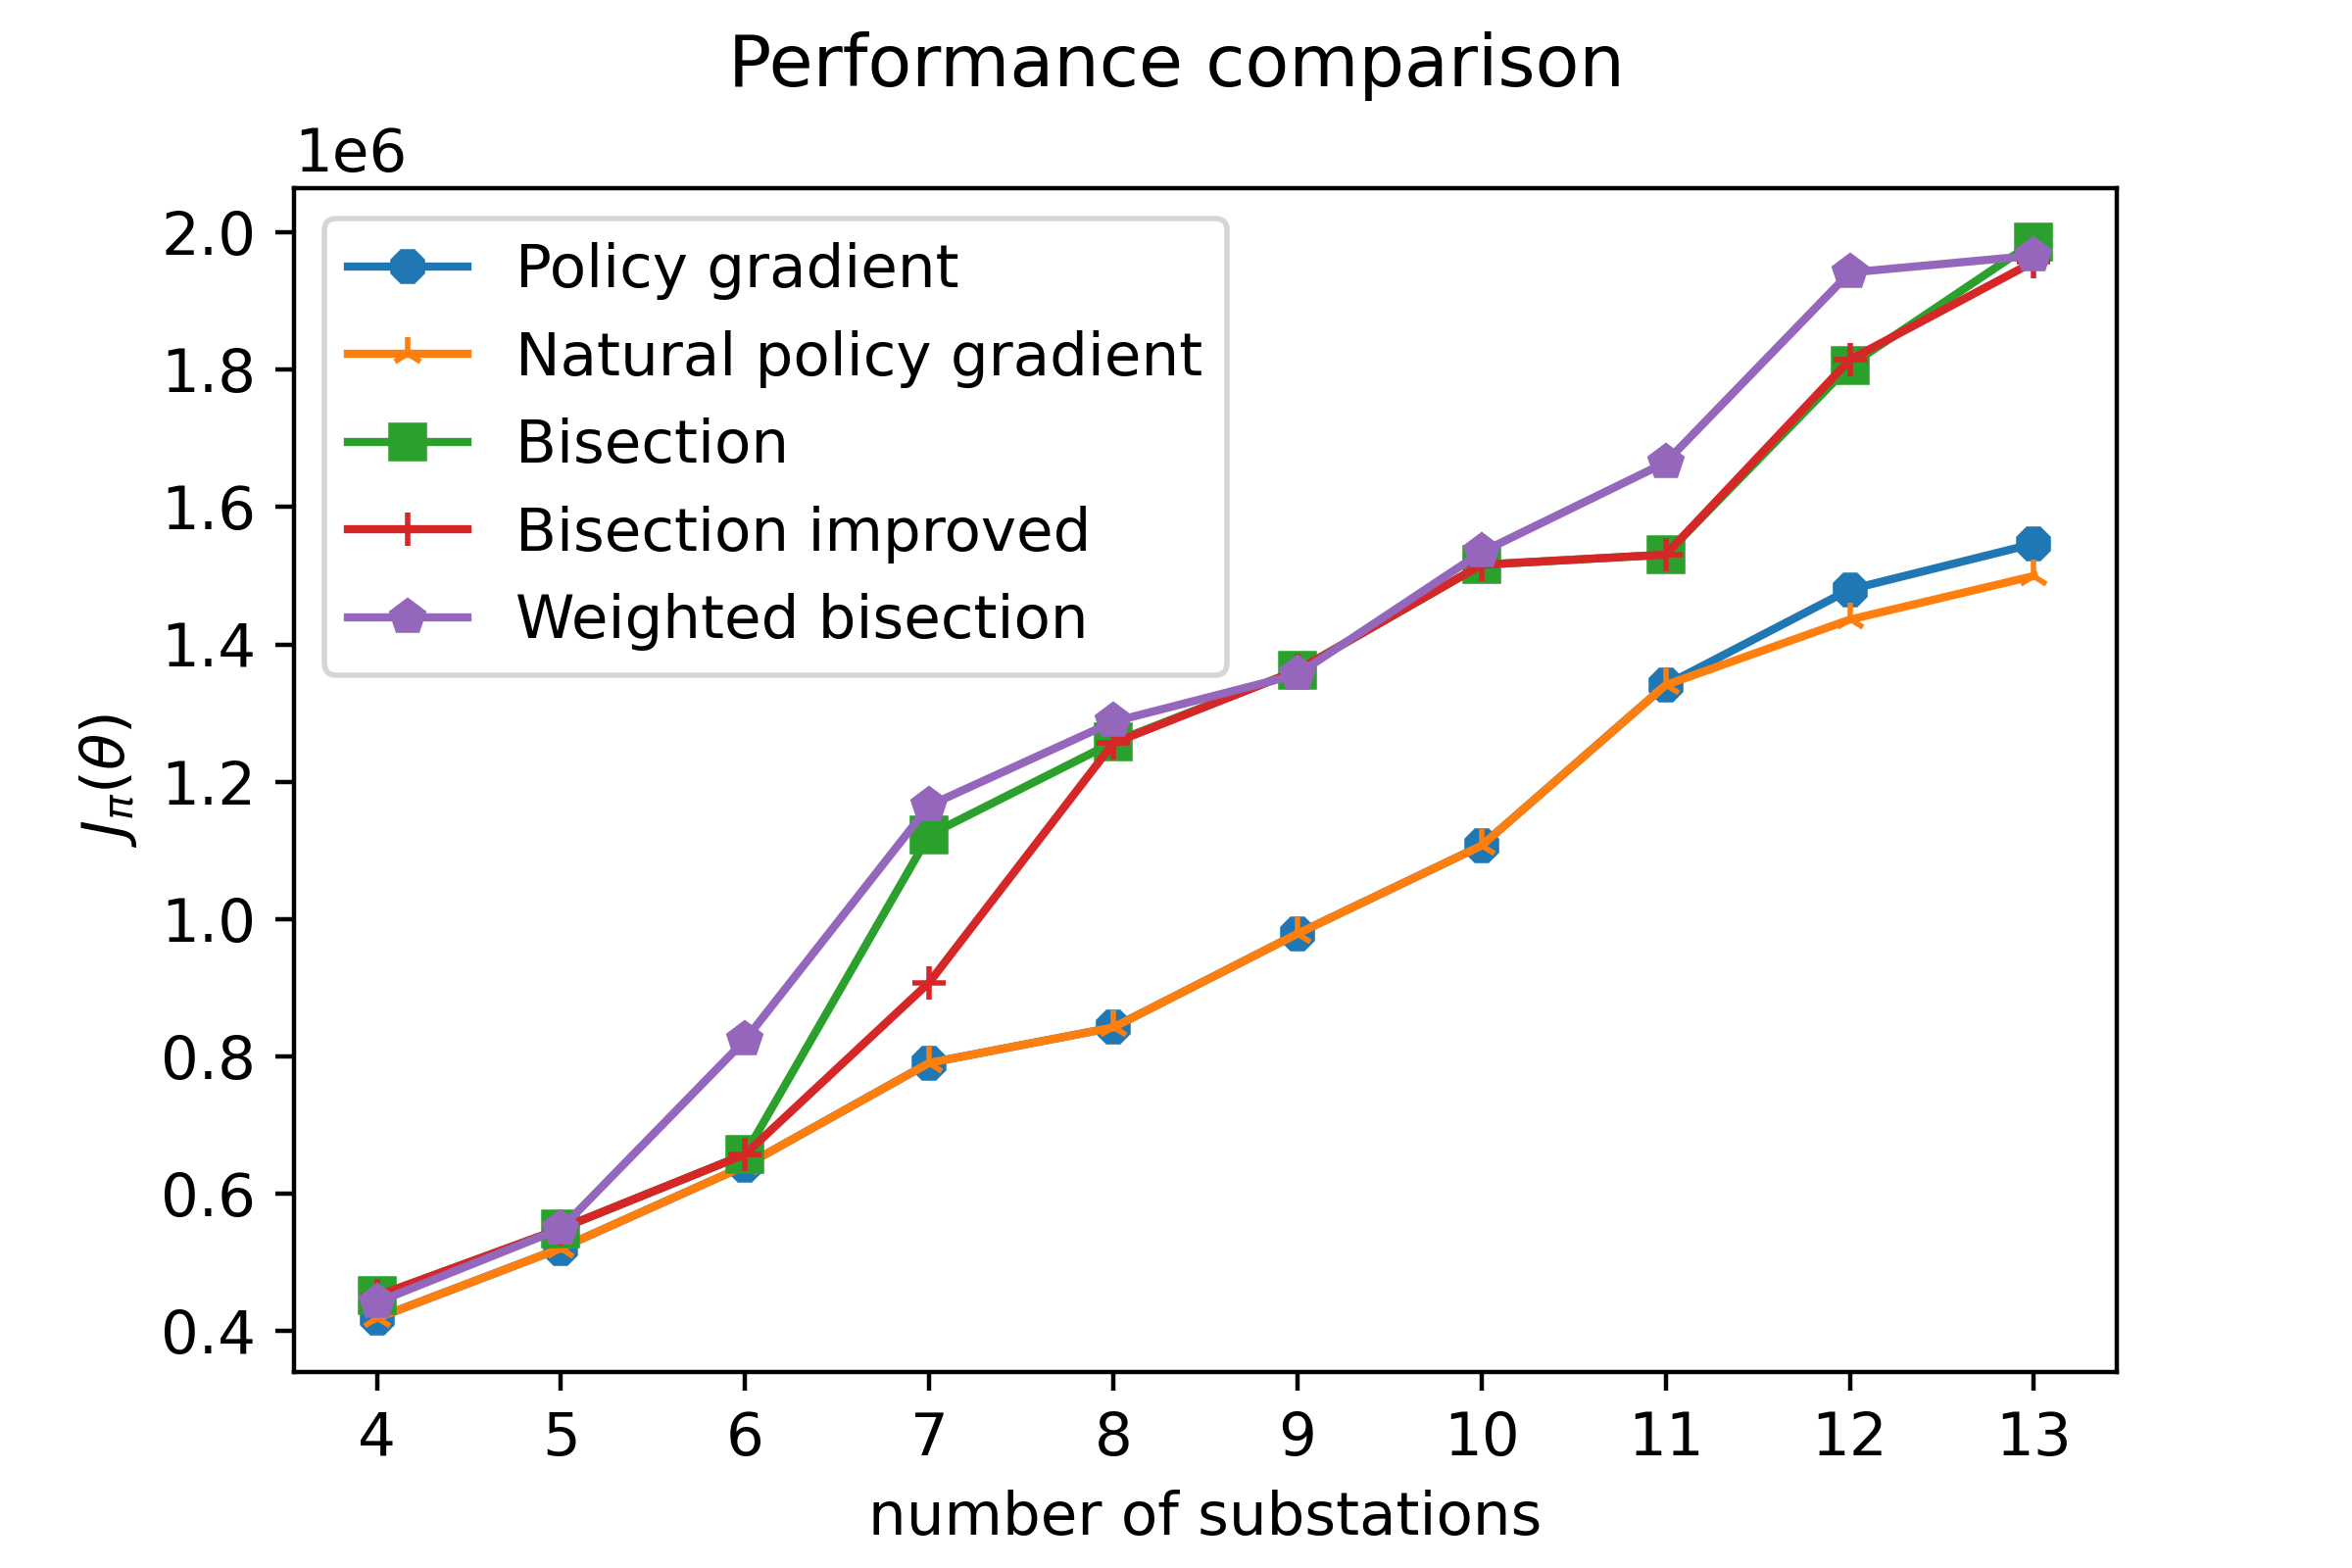
\includegraphics[width=0.8\textwidth]{chapters/figures/comparison_graph.png}
    \caption{Comparison among the various algorithm.}
    \label{fig:comparison-graph}
\end{figure}

In \autoref{fig:scatterplot} we can see a plot of the costs for different positions of the fault of the \acrshort{pg} and the bisection algorithms. We considered only the faults on the electrical cables, otherwise there would have been too many points, and since according to the data collected by the technicians they are the most frequent ones, thus they are the most representative. We have indicated with \texttt{f1} the fault between the first remotely controlled substation and the first disconnected substation, with \texttt{f2} the fault between the first and the second disconnected substations, with \texttt{f3} the fault between the second and the third disconnected substations, and so on so forth.

\begin{figure}[htb]
    \centering
    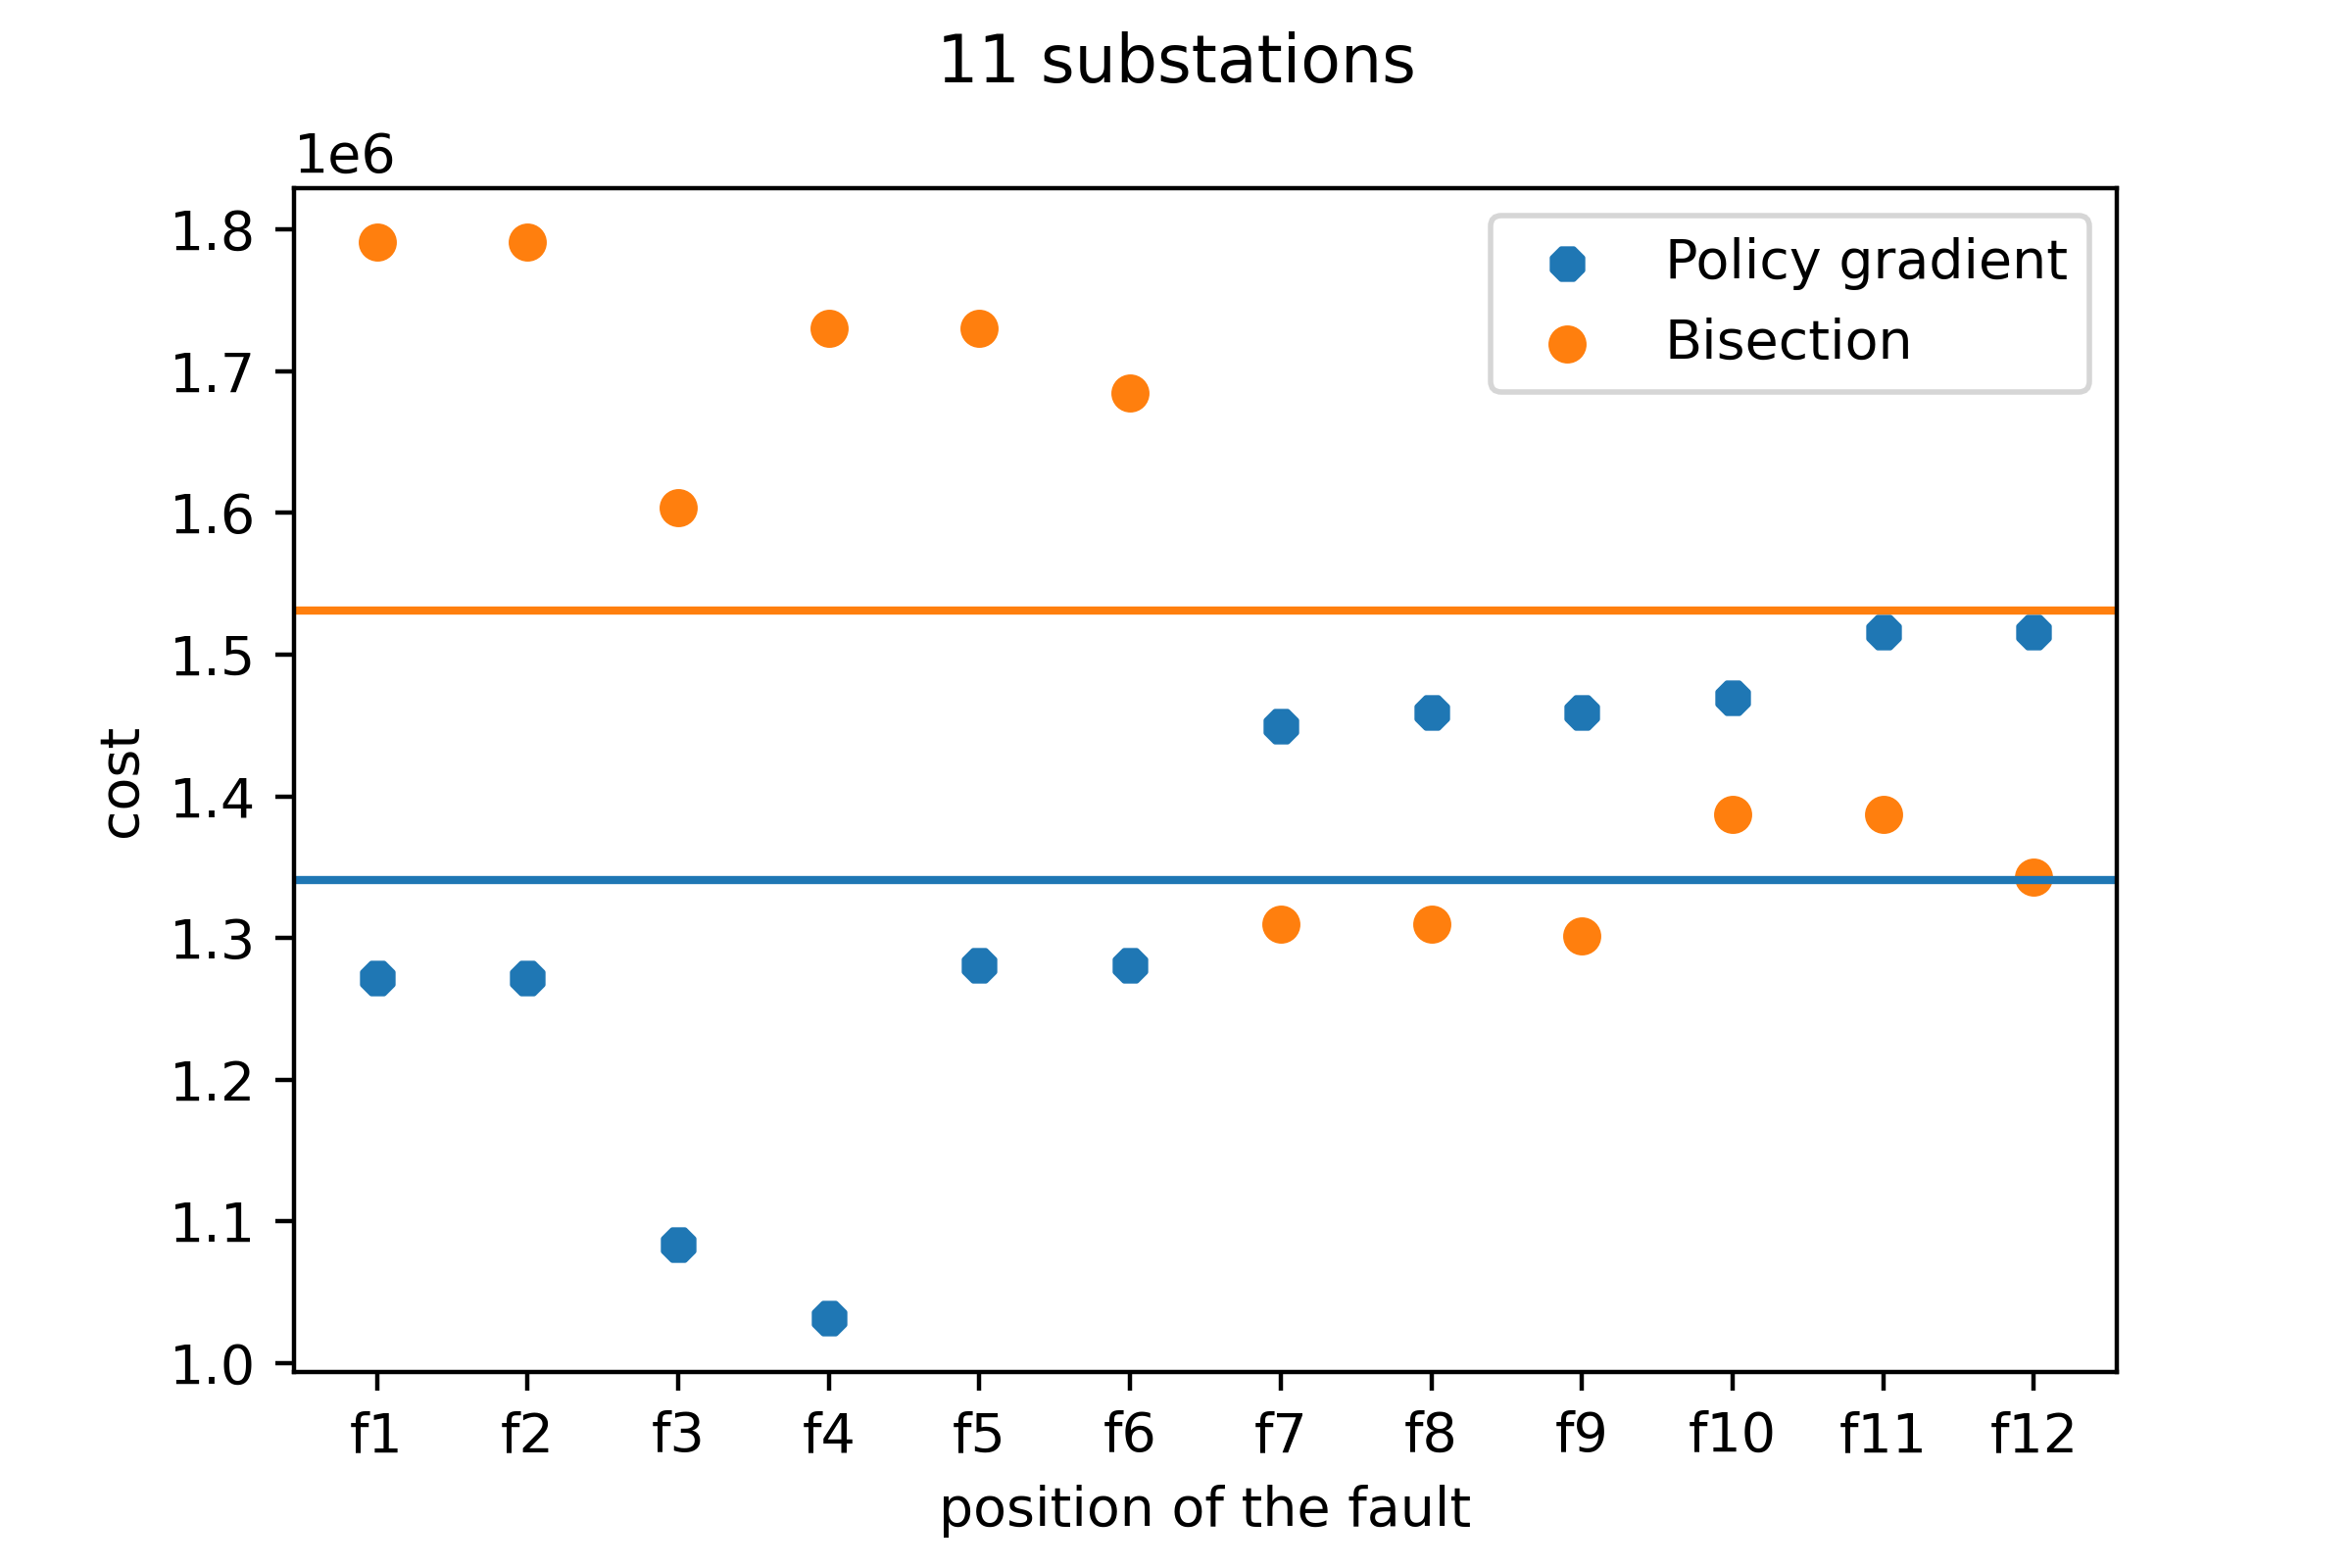
\includegraphics[width=0.8\textwidth]{chapters/figures/scatterplot.png}
    \caption{Costs for different positions of the fault.}
    \label{fig:scatterplot}
\end{figure}

\section{Conclusion}

We have succeeded in developing a method that reaches, on average, a better solution than the current one used by the technicians. But it is possible that, using a different cost structure, these results do not remain the same. The performances of the heuristic technique and the policy gradient algorithm may increase or decrease if we change the definition of the cost. However, it is remarkable that even in this case our algorithm would continue to be applicable and scalable. In fact, besides our specific results, what is important is to have developed a method that can find systematically an optimal policy in the model-based context, in which we know the consequences of our actions.

Another possible approach would be to use a model of \emph{mixed integer (linear) programming}, where only some unknown variables are required to be integers, while the others are continuous. In this case, it is possible to cerchiamo di minimizzare il caso peggiore \colorbox{yellow}{!!!!}

In real life, though, the costs are not quite like we modeled them, they are much more random, since they depend on many factors: whether it is day or night, whether the instrumental test is applicable, the weather conditions, and, of course, many other unexpected events can happen. If we are to model more accurately these costs, first of all we would have to collect data on them, using maybe a Telegram bot connected to an \acrshort{aws} server, with which the technicians can interact while solving the fault. Then a whole other class of algorithms would be needed to solve this problem: the \emph{model-free}\index{model-free} ones, specifically designed to handle these uncertainties about the costs. This would be an interesting direction for future works, but we will not cover it in the current one.